%% marcel's template

\documentclass[12pt]{article}
\usepackage[margin=0.5in]{geometry}
\usepackage{amsmath,amsthm,amssymb,amsfonts,tikz,tikzsymbols}
\usepackage[shortlabels]{enumitem}

\usepackage{float}% for making figures behave with H

\usepackage{listings}% code

\usepackage[symbol]{footmisc}% for footnotes

\usepackage{hyperref}
\hypersetup{
  colorlinks   = true,    % Colours links instead of ugly boxes
  urlcolor     = blue,    % Colour for external hyperlinks
  linkcolor    = blue,    % Colour of internal links
  citecolor    = red      % Colour of citations
}

\newenvironment{rcases}
  {\left.\begin{aligned}}
  {\end{aligned}\right\rbrace}

\newcommand{\N}{\mathbb{N}}
\newcommand{\Z}{\mathbb{Z}}
\newcommand{\Q}{\mathbb{Q}}
\newcommand{\R}{\mathbb{R}}
\newcommand{\C}{\mathbb{C}}
\newcommand{\F}{\mathbb{F}}
\newcommand{\RA}{\Rightarrow}
\newcommand\defeq{\mathrel{\stackrel{\makebox[0pt]{\mbox{\normalfont\tiny def}}}{=}}}

\newcommand{\M}{\mathbb{M}}

\renewcommand\qedsymbol{$\Smiley$}% marcel's qed symbol

\newenvironment{problem}[2][Question]{\begin{trivlist}
\item[\hskip \labelsep {\bfseries #1}\hskip \labelsep {\bfseries #2.}]}{\end{trivlist}}
\newenvironment{exercise}[2][Exercise]{\begin{trivlist}
\item[\hskip \labelsep {\bfseries #1}\hskip \labelsep {\bfseries #2.}]}{\end{trivlist}}
%If you want to title your bold things something different just make another thing exactly like this but replace "problem" with the name of the thing you want, like theorem or lemma or whatever

\begin{document}
 
%\renewcommand{\qedsymbol}{\filledbox}
%Good resources for looking up how to do stuff:
%Binary operators: http://www.access2science.com/latex/Binary.html
%General help: http://en.wikibooks.org/wiki/LaTeX/Mathematics
%Or just google stuff
 
\title{\texttt{DATA\_SILSO\_HISTO}\\Log}
\author{Stephen Fay}
\maketitle

\tableofcontents

\section{Introduction}
\subsection{Github repository and project}
    https://github.com/dcxSt/DATA\_SILSO\_HISTO\_search \\
    https://github.com/users/dcxSt/projects/2?fullscreen=true

\section{Equations}

\begin{equation}\label{derivde equation}
    r = a\cdot(10 g + b\cdot f) = 10 a\cdot g + c\cdot f
\end{equation}

\begin{equation}\label{standard deviation equation}
    \sigma = \sqrt{\frac{\sum_{i=1}^{n} (x_i - \bar{x})^2}{n-1}}  \quad \quad \quad \quad 
    var = \frac{\sum_{i=1}^{n} (x_i - \bar{x})^2}{n-1}
\end{equation}

\section{Log}

\subsection{Before The Solstice}
I only started the log on the solstice so I forgot the details of what I was doing before then. The time was spent learning the basics of \texttt{SQL} and how to interface with an \texttt{SQL} database through the mysql terminal; acquainting myself with the data and with what it is I ought to be doing. This is the period where I wrote some of the basic methods that I now use every day for accessing and connecting with the Mittheilungen.


\subsection{Friday June 21}
\begin{itemize}
    \item Today no-one was in the office in the morning so I didn't have access to the Mittheilungen journals and decided to start writing this instead
    \item at 10:20 I was let into my bit with all my notes and the journals and began 'searching the manuals' part of the project documented in the Github project linked
    \item been spending time writing in all the pink corrections, including typos
    \item started writing \texttt{searching\_the\_manuals.py}
    \item wrote and executed methods : \texttt{correct\_typos\_for\_pink()} ; \texttt{pink()}
    \item searching the manuals for all comments labeled 'uncertain' so as to figure out what is this word's range of meaning (wishing I had paid attention in German class)
\end{itemize}
    
\subsection{Monday June 24}
\begin{itemize}
    \item 9.15 picking up from where I left off, I am currently scouring the manuals for any `uncertain' data
    \item 10.40 came across some duplicate data, and mysterious comments... there are some asterisks `*' that signify a change of instrument but nothing is written. The annoying thing about the duplicate data is that it is coming from 
    \item spent the morning making that duplicate finding and sorting algorithm, now I need to analyse the nature of the problem further. For each of the duplicates identify what kind it is, weather it's the same observer with the same instrument; if the duplicated data has for example the same rubrics numbers as each other ; if they record the same information (sunspot groups, sunspots, wolf number) ; if check to see if any clues are hidden in the comments of these duplicated data
    \item in searching\_the\_manuals I wrote : \texttt{find\_duplicate\_observers()} ;\\ \texttt{find\_obs\_id\_by\_date()} ; \texttt{find\_observer\_alias\_by\_id()} ; \texttt{find\_duplicates\_data()} ;\\ \texttt{write\_greater\_duplicates\_data\_text()}
\end{itemize}
    
\subsection{Tuesday June 25}
\begin{itemize}
    \item 9.45 I have decided to start making modifications to the database, this is risky business - I don't want to have the blood of Galileo's data on my hands, in a few seconds I can destroy hours upon hours of some great astronomer's work. Which would be a shame. This is why I am creating a new table in both the old and the new database that will serve as a rubbish bin, so that I simultaneously copy and delete some data. The data will be copied and destroyed in the same script but the copying will come \textit{before} so if there are bugs nothing will be lost. First I will back up the databases as they are.
    \item While making the rubbish bins for DATA\_SILSO\_HISTO if found that DATA\_DEV was non-empty, it contains data which claims to be observations made by the grandfather of this series - Rudolf Wolf. Only the observations are dated January 1600 - Galileo's time, 216 years before Wolf's birth! And so I renamed the DATA\_DEV to RUBBISH\_DATA and added the flag column, leaving those four observations inside where they probably belong...
    \item Wrote a new script to deal uniquely with deleting the duplicates
    \begin{itemize}
        \item finished writing \texttt{move\_data\_to\_bin} and \texttt{delete\_entered\_twice\_duplicates}
        \item executing \texttt{delete\_entered\_twice\_duplicates()}... done
        \item finished commenting these data points in rubbish data in both databases
    \end{itemize}
\end{itemize}
    
\subsection{Wednesday June 26}
\begin{itemize}
    \item wrote a new method in \texttt{db\_edit} for appending comments rather than replacing them
    \item wrote \textit{unreasonable\_sn\_flag()} a method that takes a look at the groups number and the sunspots number of each entry and determines if it's realistic or not. I decided somewhat arbitrarily that if the groups number was higher than 30 it would be flagged with flag 4, if the groups number was higher than 60 it would be marked with a 5 this is beyond unreasonable. I did something similar for the sunspots number $sunspots>100\Rightarrow flag:=4$ and $sunspots>250\Rightarrow flag:=5$ (see the flags section \ref{reference to flag here}reference to flag here). The method was executed and ran without a hitch (after a bit of debugging)
    \item just set another 212 flags for putting things in the bin. There are still 4000 pairs of duplicates that need attending to but considering i started with 14000 that's not bad... Some of the duplicates may be left as they are. Also i figured out that i had flagged some which just had a 0 sunspot number and so i went and unflagged them.
    \item Scrutinised what i had flagged, reread my scripts, (noticing how inefficient my algorithms are), checking data is in the right place and taking another look at the flags.
    \item something that has been annoying me in this search is I can't seem to be able to determine what is an unreasonable number of sunspots that can appear on the sun, because many many observer record having over 250. This is why I will start using graphical tools to help me figure all of this out. I will make the graphs in a jupyter notebook.
\end{itemize}
    
\subsection{Thursday June 27}
\begin{itemize}
    \item first thing i did today is to go though and look at lots of the flagged data from yesterday on the mysql databases
    \item Panic! While searching I came across a big problem. Many of the datapoints are labelled `*' in the comments, this corresponds to when there is an asterix in the Mitteilungen journals, but here's the twist: the star is usually a reference to the fact that there is a change in the observer's telescope to his/her secondary lunette. This is written nowhere is many cases in the digital database! This is a new task I must take on am I to accomplish my mission here:
    \begin{enumerate}
        \item Correct all the comments so that they display useful information i.e. `*' $\to$ `* = 8 cm Oeffnung mit 64-facher Vergrosserung und Polarisationshelioscop'
        \item When you tackle the `Creating New Aliases' part of the project (see my Github - username = dcxSt - project sun)
    \end{enumerate}
    \item I found there I had flagged all the mysterious `*' comment 1 and that none of them have found their way into my pristine database GOOD\_DATA\_SILSO and so I went through each of them individually and wrote the changes that I implemented in the python method `correct\_asterix\_comments()' in script `db\_homogenise\_comments.py'. This took quite some time and included translating German with my good friend google-translate. This corrected about 250 data-points' comments (i didn't bother to count)
    \item after a long search of the data in GOOD\_DATA\_SILSO with FLAG=3 which have no superior duplicates I found that these were infact correctly flag and that their double had not yet made it into my new database because there were commented (usually with an asterisk *) so i moved them into the bin
    \item Found a bug in \texttt{move\_flag3\_to\_bin()} which may have been causing some of the perplexing problems I had earlier
    \item I ran the method `flag\_many\_duplicates()' many times using the duplicates text files I'd made earlier for inspiration to change it subtly so as to catch those sneaky no good duplicates!
    \item IMPORTANT: I just found some data which has been written in in the wrong year. In rubrics 820 students have mistakenly typed in the data for Wolfer in the year 1900 and written it in the year 1899.
    \item In the folder duplicates/3 2019.06.27 I am writing the file \texttt{corrections\_needed\_handwritten.txt} which outlines the corrections which are to be made to the data if we want to solve some of these duplicates.
\end{itemize}
    
\subsection{Friday June 28} 
\begin{itemize}
    \item Continued what I was writing yesterday, looking through the manuals and identifying. The notes I took about the duplicates can be found in \texttt{different\_value\_duplicates.txt}, some things I found interesting so I decided to copy most of the file into this report
    \item Carrington datapoint id=31460 needs to go in the bin this is clearly a penumbra
    \item All observations in rubric number = 808 with fk\_rubrics = 461 were made by Konkoly not Wolfer
    \item All observations in rubric number = 820 were made by Wolfer in the year 1900 and not 1899, many observations are written correctly except for the year of the date, I found that the months and days correspond perfectly with what is written in the journals but not the year!
    \item The Broger duplicates for 1899-03-17 and 1899-04-18 make very little sense, they are broger under two different aliases but in the same rubrics 801. There are only two of them so they can be done by hand. My guess is that they were punched in twice by different people and my identical duplicates algorythem has already dealt with the ones that were exactly the same, so these are the 2 instances where one of the people got it wrong.
    \item Observations in mitt 129 rubrics number 02 (or 12902) were all made by Broger in 1931. Manny if not all of them were typed in wrong, it says they were made in 1908. Thankfully everything else about them seems correct.
    \item For Rubrics 1057 and 1058 there is a serious problem - Both are labled with the wrong observer! 
    \begin{itemize}
        \item Rubrics number 1057, the observations are made in the Capodimonte Observatory by Dr. E. Guerrieri,
        \item Rubrics number 1058, the observations are made in Floreze by Robert Lucchini. I checked and both of these people are real observers with aliases, so this needs to be corrected.
        \item The reason there is confusion about these two is because Herrn J. Sormano in Turin is mentioned since the observations come from letters of correspondence between Sormano and the two observers mentioned above. It is quite possible that this has been going on in other places under the radar. The only reason these two were detected was because they just so happened to be attributed to the same guy for observations on the same date. What I propose is that we have someone (perhaps me, Asside: maybe an AI could do this if we scanned every page of the journals and then trained a neural net to read the rubrics descriptors and figure the observer based on that... This might be hard for this task but I can see how some machine learning could come in handy for error detection and quality control) go through each rubrics number and make a list where every rubrics number is ascribed to an observer, specially for the rubrics descriptors that include the names of several people, come to think of it a German person would proably do a much better job at this then me.
        \item To speculate further it is possible that this issue runs deep and that many of the holes in the data are infact a concequence of the kind of error described above (by the way I can cut out alot of my rambling from the final draght of the report, or make a condensed version, I'm just in the habit of writing everything down so that future me can follow the thought process, sometimes it helps ok!)
\end{itemize}
\item Observations from rubrics number 1279 were incorrectly labled as comming from 1919 when infact they are from 1920. The observer (Prof. Anne Young) and all other info is correct.
\item Something annoying happens in 1929, Both Brunner - `Wm. Brunner'  and his assistant - `W. Brunner, Assistent' seem to be observing at the same time [BOTH OF THEM ARE DENOTED WITH THE ALIAS `Brunner'] with the same 8 cm aperture 64x magnification polarised helio-telescope. Rubrics 1624 (fk\_rubrics=840) is Brunner and his assistent's observations are from Rubrics 1675 (fk\_rubrics=842). I don't know what we should do, perhaps create another alias 'Brunner Assistent' (pink page marker)
\begin{itemize}
    \item Same thing happens in rubrics 12501 (fk=844) is the real Brunner, and rubrics 12503 (fk=846), this is Brunner Assistent (yellow page marker).
    \item Same again in 1931. Rubrics 12901 (fk=848) is the real Brunner, and rubrics 12903 (fk=962), this is Brunner Assistent (orange page marker)
    \item ...This goes on until (see the file for details)...
    \item And in 1944. Rubrics 14401 (fk=1006) is the real Brunner, and rubrics 14402 (fk=1007) is Brunner Assistent. (green page-marker on page 112)
    \item Comments on Brunner: I'm annoyed that the assistant(s) doesn't have a name because we now have no idea how many there where. Also (s)he deserves credit for those 10 odd years of commited observation! Because this assistent has been observing with Brunner from 1929 to 1944 he at least deserves an alias. 
\end{itemize}
\item Messerschmitt and Wasnetzoff
\begin{itemize}
    \item Something strange happens with Messerschmitt, there are two different sunspots values written in for 1908-02-15, one of them has no rubrics number and values 3,17,47 The other has a rubrics number 1028 and values 2,7,27. So I looked in the journals under rubrics 1027 and for this date I found the values 3,17,47 which are the values written in where no rubric is specified. Very strange. There are a total of 4 duplicates for Messerschmitt and this is the only one that has a rubrics number. I find this very strange... I don't really know what to do. 
\end{itemize}
\end{itemize}
    
\subsection{Monday July 1}
\begin{itemize}
    \item Using what I did on Friday (wrote that list of things that were wrong with specific duplicates) to bin some data and modify other data
    \item Started writing methods \texttt{flag3\_from\_correction\_txt()} and \texttt{change\_rubric\_observer()} and\\ \texttt{change\_date\_rubric()} in \texttt{dealing\_with\_duplicates.py}, and then I realised that all this was much simpler and could be done faster and less error prone if I just punched in the queries to through mysql directly, so this is what I did.
    \item With care and delicacy I changed the observer aliases / and for the old and bad database I changed the FK\_OBSERVERS with the terminal. Now I move onto changing all the faulty dates, this requires a bit of coding because I need to loop through the dates and change each date individually.
    \item Wrote \texttt{change\_dates()} and it's helper \texttt{change\_date\_rubric()} (in \texttt{dealing\_with\_duplicates.py}) and executed them in more time than it should have taken. My head is not clear today, but I was rigorous, there should not be a mistake.
    \item I am changing the databases quite a bit so I saved a new backup file
    \item made a new alias in \texttt{DATA\_SILSO\_HISTO} (and \texttt{BAD\_DATA\_SILSO}) called `Brunner Assistent'. I know the name lacks imagination but hey (I couldn't find who it might be online - future me : this is a reminder to ask Frederic if he might know, be ready with dates...).
    \item I just realised that when I was changing some of the data in \texttt{GOOD\_DATA\_SILSO} I only changed the aliases, to correct this I will either write now or once everything is finished a method that goes through each data-point finds the alias and corrects the observer data (things such as the country of observation, the observer comments and the instrument etc.)
    \item wrote and executed the command in \texttt{dealing\_with\_duplicates.py} \texttt{change\_alias\_to\_brunner\_assistent()}, this corrected the brunner assistent problem we had
    \item backed up the the databases to sql files
    \item I realised that I had missed correcting the alias for rubrics 195 from Franzenau to Weber so I did that just now
    \item Ran the method that shows me what is wrong with the duplicates to see how effective my cleanup has been : interesting, the duplicates that were Weber's but marked Franzenau had already been entered under Weber but with rubrics\_number=0 and no references in the Mittheilungen, so I reran the \texttt{flag\_many\_duplicates}.
    \item Some of the `Tacchini and Milesovich' are missing sources but the duplicates are identical, so I moved one from each to the rubbish bit by calling the method \texttt{delete\_entered\_twice\_duplicates()} from \texttt{dealing\_with\_duplicates.py}. There was also the issue that Broger had some identical data typed in for him in two using two different observer ids that both refer to him... so i added a conditional (elif) statement into the delete entered twice duplicates method to deal specifically with this.
    \item Most of this data has been cleaned up, the rest can be done by hand
\end{itemize}
    
\subsection{Tuesday July 2}
\begin{itemize}
    \item exploring ways of creating visualisations that will help me catch some of the suspicious data-points. Right now my task is hunting down those ones which I labelled 'suspicious sunspots'
    \item made some pretty plots which you can find in \textit{suspicious sunspots plots.ipynb} in the root directory
    \item Using the plot I was able to check some of Weber's suspicious sunspots in the Mittheilungen. And strangely enough Weber's observations are correct! It seems he really did see 476 sunspots on the sun on the 25th of september 1870. I mean the pattern fits it's just unsusually large. And you need to be dedicated to count hundreds of spots every day.
    \item Made a method in the jupyter notebook mentioned above that plots an observer's stuff and color codes the flags. I investigated Tacchini's green (flag=4) datapoints and they are infact correct, they appear in the journals. There is one datapoint from Tacchini which I corrected by hand, this one had a wolf number of 61, I found it in the journals, the correct value was 6 - typo. I corrected it manually.
    \item In the rubric 279 mitt 30 page 409 Tacchini observes a bunch of sunspots without observing any groups. This is annoying because it means we have no wolf! Other than that they seem to have been entered in correctly, I have not yet transfered these to the \texttt{GOOD DATA SILSO} database, they are still only in \texttt{DATA SILSO HISTO} and \texttt{BAD DATA SILSO}
    \item I have an idea that we could do some stats and deduce a wolf number even without the groups, and give it a special flag, based on some probability we estimate a wolf number. There might be some complications with this tactic, here are 3 possible ways of doing it and their weaknesses:
    \begin{enumerate}
        \item For each sunspots number possible \{1,2,3...\} find the corresponding most likely wolf number by going though each data point with that number and doing a distribution (probs normal) to find which is the most likely wolf number associated with this sunspots number. Essentially we define a function term-by term $f \defeq{} \N \to \R$. The weakness : if we sample everything we might find that Tacchini has his own idiosyncratic way of doing sunspots and wolf, and so the data we add to his entriee would not fit well with his methods of observation.
        \item For each sunspots number do the same as above but go through the groups number! Again for each sunspots number sift through all the data of everyone to find the best groups number $g\in \R$, i.e. the $g$ s.t. it sits on top of the fitted normal distribution.
        \item For each sunspots number, methods 1) and 2) above but fitted with only Tacchini's previous and future data. The weakness of this method is that there is not much data to go on... (relative to the first two)
        \item One thing that worries me in the case of Tacchini is that this guy observers a lot of sunspots. I am looking at his entries right now and in 1870 he regularly observers over 200 sunspots, on $5^{th}$ of April 1870 he sees 302 sunspots. That said cross-referencing his data with other observers' from the same time seems to support this hypothesis. But the more sunspots he observers, the less data we have to make a nice normal distribution for each sunspots number, there may be sunspots numbers that only appear like 3 times in the whole database, how are we to do any stats on those. The answer is the following method for tying sunspots to groups and wolf number: for each sunspots number we link it to a wolf number by finding the best fit normal distribution for the likeliest wolf number to be associated with it. Then we give this value an error bar which is bigger the less data we have. Then we do a plot x-axis = sunspots number, y-axis = wolf numbers with vertical error bars. Then we do a line of best fit through the whole lot, try several models and do a chi-squared test. It might be worth getting rid of the small ones and only look at data where $s>20$. Again we could do this for wolf directly and for groups then wolf.
    \end{enumerate}
    \item Before embarking on this adventure I will first endeavour to plug both of Tacchini's hole's that appear in the plots I made: 3 entire years are missing From Tacchini's data 1877, 1878 and 1881
    \item In 1881 the rubrics number 465 contains two data sets, one of them is entirely Ricco's and the second is from Tacchini and G. Millosevich. Nowhere in the data set is it indicated who saw what, so I looked and found that there was no Alias for Millosevich. This makes me think that he must be Tacchini's assistant or observing partner. Anyway we have a big gap in Tacchini's observations, what I will do is comment all of these observations ``Tacchini and Millosevich". I did that and gave them a flag, then regenerated the Tacchini graphs and there is no more gap in 1881, what's more the data looks almost identical. There is one only slightly worrying difference and maybe I'm inventing patterns where I am trying to see them but the 1881 observations are on average a tiny tiny bit higher than the surroundings. Looking closer at the picture, I think this is infact a seasonal effect, there is more atmosphere...
\item I improved the jupyter notebook ``suspiciou sunspots plots.ipynb", made a cool colour scheme for the various flags.
\end{itemize}
    
\subsection{Wednesday July 3}\label{wed 3 jul}
\begin{itemize}
    \item Precisely the same thing happens to Tacchini in 1877 and 1878 but this time it is ``Tacchini und G. De Lisa". I did the same as yesterday: changed the information so that it was no longer in the observer and alias but commented instead, and flagged it with flag 6 (\textit{edit: later this was changed to flag 3 with the new definition})
    \item Found outlier for Tacchini, ID=46145, Mitt 30 Page 410 Rubrics 279 date 1871-04-12. Error type = typo. For groups wrote 112 instead of 12. 
    \item I wrote some methods in \txttt{graphs\_helper.py} mainly for helping me to display data in jupyter notebooks while avoiding over-saturating my jupyter notebooks.
    \item The reason I've gone off track from the github project objectives is frankly because I was getting board of scouring the manuals for ages, but my enthusiasm for this task has regenerated now and this is what I will do. Once the errors from the \texttt{sorted\_greater\_comments\_list3} have been fully dealt with I'll throw myself back into hunting for errors via graphic visualisation. And perhaps implement that idea I had yesterday about doing some stats on the relationships between sunspots, wolf and groups numbers (if I do this I estimate it will take around 4 days, which is quite a lot considering I usually underestimate these things, since it is not crucial to what I am doing I am considering doing this in my free time on the weekend perhaps...)
    \item Modified some Quimby comments, there was two stars int the rubrics 706 which had no explanation, I modified these two comments `*=secondary telescope' and flagged them with flag 6. There is no point in making a new alias because so few of his measurements are made with his secondary telescope, perhaps we should just get rid of them...
    \item Realising that I was making inefficient use of my time, I am now going through all the data with \texttt{COMMENTS}=`uncertain' where I have manually checked in the Mittheilungen manuals and changing them with the following query: \texttt{UPDATE DATA SET COMMENT='?',FLAG=2 WHERE FK\_RUBRICS=XXX AND COMMENT='uncertain';}. Since all of these were flagged initially because I didn't know what to do with them, they all find themselves in the BAD\_DATA\_SILSO so I also execute \texttt{UPDATE BAD\_DATA\_SILSO.DATA SET COMMENT='?',FLAG=2 WHERE FK\_RUBRICS=XXX AND COMMENT='uncertain';}. Once I have finished with these they will all be moved to the good database that selects things that have flag=2 and moves them.
    \item It may well be written at the beginning of one of the Mittheilungen, but I have not yet found what the `?' comment means. I have two theories.\label{what is flag 2 question mark}
    \begin{enumerate}
        \item I noticed the question-marks appear in Mittheilungen where there are several observers, in-fact I have not yet found a rubric where there are question-marks but no second observer / telescope. So I suspect it might be that Mr Wolf (or whoever wrote the journals de Mittheilungen) is unsure as to who took the measurement. CORRECTION: I found one where there is no secondary telescope or observer - rubrics 779, observer = Winkler, mitt 90, page 326. There is only one telescope and one observer, yet there are still question marks.
        \item My initial suspicion before I noticed 1. is that the question-marks denoted observations that were made on a cloudy day - or the measurement was somehow obfuscated. Oooh! I think this is right, but still not sure for every observer... There is written rubrics 1081 Herm. Kleiner writes ``? bedeutet schlechte Definition des Sonnenbildes" - \textit{? signifie mauvaise définition de l'image du soleil}.
    \end{enumerate}
    \item On second thoughts there are alot of red comments, I think it will take the rest of today (the next 4 hours) to verify every one of them in the journals and take note of them. I will do this and then write a script that changes their comments and flags all at once.
    \item I updated DATA in all databases with \texttt{UPDATE DATA SET COMMENT=`?=bad definition of sun image',FLAG=2 WHERE COMMENT LIKE `mauvaise d\%';}
    \item Found some comments where there is both an observer and a question mark at the same time, for these ones I left the comments as they are and changed only the flag from 1 to 2.
    \item In rubrics 1037 mitt 100 page 359, observer `Ricco - Mascari', there are two data-points with comment `0 0'. I checked the values in the journal and they were wrong! There are corrections I made
    \begin{enumerate}
        \item 1908-10-17 groups 0, sunspots 18, wolf 18 (impossible) $\to$ groups=0, sunspots=0, wolf=0, comment='', flag=0
        \item 1908-11-17 groups 0, sunspots 18, wolf 18 (impossible) $\to$ Deleted - there is no observation made on this date in this rubric
    \end{enumerate}
    \item I spotted a missing value in rubrics 12904 observer Buser for the observation on 1931-03-10 whilst I was correction the previous day's which was incorrect, so I entered it in. There may be more here in this rubrics.
    \item Now I finished looking at the red comments (I still need to change them and move them all with python, that should only take about 30 mins to copy down all the rubrics numbers into a list and write the algorythem that changes them appropriately, I will do it tomorow.) Right now I am looking through the last two pages of the comments sheet I printed and there are alot of blue ones where the comments are just numbers, these require my attention.
    \item I looked up all the blue comments on those last two pages in the journals here is a summary of my findings:
    \begin{enumerate}
        \item Some of the numbers actually pointed to the real values of the data i.e. the data had incorrect sunspot values and the comments had the correct ones. I modified these appropriately. In these cases often there was no groups but there were sunspots.
        \item some of the number were the correct values but the data was also already correct, here I just deleted the comment and removed the flag.
        \item some of the numbers were very perplexing and I have no idea what they were doing there. I just removed the flag here.
    \end{enumerate}
    \item I am going home now but I leave on a cliff hanger: the blues are almost done and I am currently investigating the mystery of `x' which appears in the data section in the journals of mitt 33 page 120 rubric 296. It was called to my attention by a comment also denoted `x'
    \item Actually I will save a new backup of the sql databases before I leave since I edited them quite a lot today.
    \end{itemize}
            
\subsection{Thursday July 4}
\begin{itemize}
    \item I did not find an explication for the mysterious `x'... Sachen has really got me here. I translated all the text surrounding it and nowhere do they explain why there is an x. Fow now I will leave it. It will probably stay in the \texttt{BAD\_DATA\_SILSO} database
    \item I have been looking into Carrington's case and here is what I found. Everything from rubrics 303 is the total area of either ther penumbra or the umbra. I will investigate further.
    \item I updated the flag 7 to ``derived from area-measurement" and flagged all of Secchi's sunspot values that were derived from the penumbra and / or umbra.
    \item Moved Secchi's derived from \texttt{BAD\_DATA\_SILSO} to \texttt{GOOD\_DATA\_SILSO} using the method \\\texttt{derived.move\_7\_to\_good()}
    \item There was a typo in some of Carrington's data which I corrected, I then transferred it into \texttt{GOOD\_DATA\_SILSO} so that it could be with it's friends
    \item For some reason the script \texttt{dealing\_with\_duplicates.py} has in it a bunch of method that are really more general that just dealing with duplicates. Because other methods inside the script depend on these I don't want to delete them, so I copied the tree following methods into \texttt{db\_transfers.py} : \texttt{mod\_data\_to\_bin()} with helpers \texttt{transcribe\_info\_old()} and \texttt{transcribe\_info\_new()}
    \item I modified \texttt{db\_transfer} so that you have the option to copy instead of swap
    \item Spoke to F. Clette about the possible conversion from the `aire' to a sunspots number. Told me to look in the mitt.
    \item Excitement! I found on page 131 of Mitt 31-40 written after rubrics 299 a description of how the author (I think R. Wolf himself) derived a formula for turning Secchi's `aire' into a sunspots number
    \item \ref{converting the `aire'} here what is written in German and Italian, with a translation in English.
    \item Tomorow I will fix Carrington's data, but before doing that investigate all of these : \texttt{SELECT * FROM RUBRICS WHERE RUBRICS\_ID IN (SELECT FK\_RUBRICS FROM DATA WHERE FK\_OBSERVERS IN (36,49));}
    \item Made a new backup of databases.
\end{itemize}
        
\subsection{Friday July 5}
\begin{itemize}
    \item I was searching all of Carrington's data from different rubrics in order to see if I could find an overlap in time from data where there is recorded the `air' and data where there is recorded the sunspots number. Some of the groups number seem to conflict...
    \item This is very perturbing, the groups number for rubrics 199 (Carrington) does not seem to agree with the groups number for rubrics 303 (also Carrington), however they are very similar. The only explanation I can think of is that in 303 Carrington writes number\_of\_big\_spots.surface\_area and in rubrics 199 he simply write groups.sunspots. I am still hunting for clues in the text \ref{rubrics 303, carrington}. This theory is evidenced by the fact that the number of big spots is always bigger than the number of groups which you would expect were it true.
    \item The thing to do now is graphs. I will make graphs to try and figure it out.
    \item Found one typo in the data id=31372 and corrected it
    \item Made the notebook \texttt{carrington\_investigation\_groups.ipynb}
    \item Missing data: while trying to analyse carrington's strange behaviour I cross reference every date from rubrics 199 with dates in 1859 and 1860 from 303 and found 7 missing data-points which I looked up in the journals and 4 of them were in there. So I hand-typed them into \texttt{DATA\_SILSO\_HISTO} and then copied them over into \texttt{GOOD\_DATA\_SILSO} with the method \texttt{db\_transfers.db\_transfer(dont\_delete=True)}. They are :
    \begin{itemize}
        \item rub 303 1860-08-07, ID = 206774
        \item for 1860-10-07 and 1860-11-16 there is nothing in rubrics 303, perhaps Carrington only did the sunspots number those days
        \item rub 199 1860-09-15, ID = 206775
        \item for 1860-10-08 there is nothing in rubrics 199, perhaps Carrington only did the penumbra for this day
        \item rub 199 1860-10-28, ID = 206776
        \item rub 199 1860-12-10, ID = 206777
    \end{itemize}
    \item I did a comparison of the groups number from rubrics 199

\item I have a problem, in order to implement the modifications I would like to make to Carrington's rubrics 303 data I need the groups, sunspots and wolf all to be floating point numbers, right now in the database they are integers and I cannot modify them as such.
\item I found a relationship between what is labelled groups and the actual groups number for rubrics 303, see \texttt{carrington\_investigation\_groups.ipynb}
\item These are my suggested modifications : do as the author of rubrics 299 did for Secchi (\ref{rubrics 299, secchi}). However I can do better, he did not have the power of computers and he makes many approximations that are not needed today. For instance, he takes the mean from each 20 equations out of his set of 120, there is no need for this today. I will on the other hand draw inspiration from him on his model:
$$r = a\cdot(10 g + b\cdot f) = 10 a\cdot g + c\cdot f$$
according to him it fits quite well.
\item In order not to disrupt the database I have decided to sacrifice a smidgen of accuracy in order to keep using integers for the $r$, $g$ and $s$ (wolf, groups, sunspots). ($f$ is the `aire'). I will do the following things (see \texttt{carrington\_investigation\_wolf.ipynb}):
\begin{enumerate}
    \item Basing myself off of the relationship described by equation (\ref{derivde equation}) I will do a least squares fitting as I did for the groups, to find values for $a$ and $b$
    \item I will then do the same least squares fitting using a modified $g$ which I have multiplied by a factor of $\frac{1}{1.0915}$ to see if the standard deviation is at all better for this group
    \item If the fit is not as good as hoped I will try several other models to see if I can find an equation (with maximum 3 or 4 degrees of freedom) which fits the data well
    \item From my model I will the deduce $s$, the corresponding sunspots number which, when combined with $g$ gives $r$
    \item Using my newly found equations and constants I will then apply modifications onto the rest of rubrics 303
    \item I will then round $g$, $s$ and $r$ to the nearest integer and enter these into the database.
\end{enumerate}
\item Something Sabrina brought to my attention was that my training group is only 2 years long, during a maximum, this might mess with the results a little bit.
\end{itemize}

\subsection{Monday July 8}
\begin{itemize}
    \item I have been editing my 2 reports in the morning
    \item \texttt{carrington\_investigation\_wolf.ipynb} Realised that modifying the groups was useless because I would be dividing them 1.01, so I'm skipping step 2 (last Friday)
    \item Judging by the visuals I don't need to do step 3, also it would be risky because as Sabrina said I don't have any data close to 0.
    \item Plotted carrington's data
    \item Lunch
    \item Created new rubrics id (fk=1010) in \texttt{DATA\_SILSO\_HISTO}, this one has the same rubrics number as fk=175, \texttt{RUBRICS\_NUMBER = 303}, but it is for storing the derived carrington.
    \item Pickled the dictionaries used in \testtt{carrington\_investigation\_wolf.ipynb} in cause they become inaccessible as I change rubrics 303 in \texttt{GOOD\_DATA\_SILSO}
    \item My scripts are getting very messy to work with, this is slowing me down alot. Once I have finished with Carrington I will start making that list of all the scripts and what they contain.
    \item Moved rubrics 303 from \texttt{DATA} to \texttt{RUBBISH\_DATA} in \texttt{GOOD\_DATA\_SILSO} using \texttt{db\_transfers.move\_data\_to\_bin\_only\_good()}. This required some very slap-dash patching. I'm going to look up what sort of diagrams there are out there to keep track of what is in each of my scripts, this is not very professional...
    \item I realised also that about half the methods I write I only write once, the reason I wrote them as methods is in part to keep track of every operation I performed but it is also annoying because I end up with a bunch of methods that are really in the wrong place. These ought to have been written in a jupyter notebook, or deleted.
    \item Successfully inserted the derived 303 into \texttt{DATA\_SILSO\_HISTO} with the rubrics id = 1010 instead of 175 using \texttt{db\_edit.insert\_old\_format()}. No apparent errors.
    \item Copied all those from rubrics id 1010, rubrics number 303 into \texttt{GOOD\_DATA\_SILSO} using \texttt{db\_transfers.db\_transfer()}. 
    \item I realise that there are duplicates now in \texttt{GOOD\_DATA\_SILSO}, sooner or later I may bin the derived data from rubrics 303 that overlaps with the 199 but I will first seek consultation from Laure. In-fact I think the wisest thing to do might well be to split carrington into two observers : `Carrington' and `Carrington derived'. But this creates an imbalance in the sunspots number because we are lending extra weight to Carrington for the years 1859 and 1860.
    \item I just spent the last half hour cleaning up the databases after a jupyter notebook imported an old version of on of my scripts which put into the rubbish bin all of the data with comment like `\%erive\%' in \texttt{GOOD\_DATA\_SILSO}...
    \item Just realied that I have entered in all the carrington's with the same date!
    \item I fixed it with SQL commands, it surprisingly didn't take any time at all.
    \item Saved the databases
\end{itemize}

\subsection{Tuesday July 9}
\begin{itemize}
    \item Before moving back to the comments, I'm going to apply the same fix to Kew that I did to Carrington. The bad news here is that I don't have any real data for Kew that I can compare his penumbras to. The good news is that the author of rubrics 306 already did the work for me and has found $a = 0.763$, $c = 0.032$ $\RA b = 0.042$
    $$r' = 0.763 \cdot (10 g + 0.042 f)$$
    \item Opened new jupyter notebook \texttt{kew\_derivation.ipynb}
    \item Imported and changed Kew's data according to the formula provided.
    \item Pickled Kew's penumbra data \texttt{kew\_penumbra.pickle} as well as his corrected data \texttt{kew\_derived.pickle}
    \item Made new rubrics id (fk=1011) in \texttt{DATA\_SILSO\_HISTO} for differentiating Kew's derived data from the penumbra data which I will not just scrap (alot of hard work was put into getting those).
    \item Checked that none of Kew's data had found it's way into \texttt{BAD\_DATA\_SILSO}
    \item Moved rubrics 306 from \texttt{DATA} to \texttt{RUBBISH\_DATA} using \texttt{db\_transfers.move\_data\_to\_bin()} in both the databases \texttt{DATA\_SILSO\_HISTO} and \texttt{GOOD\_DATA\_SILSO}.
    \item Inserted the derived 306 into \texttt{DATA\_SILSO\_HISTO} with rubrics id = 1011 instead of 177 using \texttt{db\_edit.insert\_old\_format()}
    \item Copied all those from \texttt{DATA\_SILSO\_HISTO} with fk\_rubrics = 1011 into \texttt{GOOD\_DATA\_SILSO} using \texttt{db\_transfers.db\_transfer\_transfer()}
    \item Saved databases and commit to github
    \item Lunch
    \item Wrote \texttt{create\_readme.py} to automatically write a long readme that tells you what is in each python file as part of an initiative to make my work available to people other than me.
    \item Cleaned up the log some more so that Laure can hopefully make some sense out of it (fingers crossed)
    \item Finnished condensing the log
    \item I just had a great idea: In the spirit of forward thinking start designing the way you are going to present the changes you have made to the data, brainstorm:
    \begin{enumerate}
        \item Explanation of new format
        \item put the log after the tables and figures
        \item Section 2 should not be called setup call it something that makes more sense, Section 2 should be for these things i am listing here
        \item Pie chart with the number of data points that have remained the same and the ones I have changed and the ones I have added
        \item Pie chart that shows what kind of modifications I made
        \item Review the explination of the flags, make it more complete yet still concise
        \item More figures that demonstrate how I have modified the database
        \item A concise list of all the things that were wrong with the database and the changes I made, this can be put in a conclusions section that I will make hereafter
        \item Should probably get rid of the thought repo
    \end{enumerate}
\end{itemize}

\subsection{Wednesday July 10}
\begin{itemize}
    \item Today was bring your Arnaud to work day. Sabrina gave Arnaud and I a tour of the observatory in the morning and I showed him what I was doing and he explained to me some cool quantum stuff as well as some EM stuff and some add cal, divergence and curl stuff... 
    \item Unfortunately I didn't do any work, I will get cracking at lunch time and stay until 18.00.
    \item After lunch I had a look at the Github project manager and realised that Carrington and Key were only an intermission in searching the manuals, and that before I have another look at some diagrams and graphs I must finish scrutinising the greater comments list 3 (i.e. `searching the manuals')
    \item I went back to Sachen's mysterious comment = `x'.
    \item I just realised that `sachen' means `things' and that `Niedersachsische neue Zeitungen von gelehrten Sachen auf das Jahr 1730. Hamburg in 8' means `Lower Saxon new newspapers of learned things to the year 1730. Hamburg in 8.', and that the existence of the observer with alias `Sachen' is most likely the student who typed this in having miss-interpreted the cryptic German capitalisation of Random Nouns, in rubric 296.
    \item There is however only data from 1730 in this rubric and I think it best to leave it be. The mysterious x is still just as mysterious, It either means 0 sunspots and groups, or missing observation ; if it's the former they should have put 0, and if it's the latter then why even bother entering in the date... Probably safer to throw away than to keep, this is something I would consult Laure about but I fear she is very busy at the moment.
    \item After some deliberation I decided to change the flags of these to 6, and let be these ones in \texttt{BAD\_DATA\_SILSO} where they shall remain, and for the ones in \texttt{DATA\_SILSO\_HISTO} to just set flag to 6.
    \item I came across my friend Carrington while scouring the blue comments (blue is the color I use for miscelaneous comments), and looking at his data I thought more about what I should do with him, and I think more and more now that it is a good idea to separate out Carrington's observations into two distinct aliases `Carrington' - for rubrics 199 and `Carrington-derived' - for rubrics 303. As for Kew perhaps renaming him to Kew derived.
    \item Oh shoot I just remembered that I had planned to make a little summary of what I was doing for Laure yesterday. I will do that now in a short email. Done
    \item I implemented the changes, there is now an alias called `Carrington derived' fk\_obs=192
    \item Some of Secchi's data is marked with a $1/2$ in the comments
    \item It seems I have just uncovered some more sunspots numbers that need deriving. These ones appear to have been hiding from me and staying under the radar due to the fact that they were measured around the years 1877, this is near a minimum so the `the column 'Area mm quadrati' in which one unit should correspond to 21.56 millionths of the area of the solar disk.' could easily be mistaken for real sunspots number. Good thing there was written $1/2$ in the comments
    \item First I cross referenced with rubrics 299 to see if the scales were the same.
    \item rubrics 299: $$f = \frac{1}{46352.5} = 2.157\cdot 10^{-5}\quad \text{solar disks}$$
    \item rubrics 375: $$f = \frac{21.56}{10^6} = 2.156 \cdot 10^{-5}\quad\text{solar disks}$$
    \item Yes they are the same! So I can use the same conversion rates that are derived in rubrics 299 for rubrics 375. Unfortunately, because of the way the wolf number is calculated it is not the case that the correction gets more accurate with smaller wolf numbers, infact I suspect that the inverse is true and that the smaller the aire, the bigger the $\sigma$
    \item Typo in rubrics page number which I corrected, there is not page 319 it goes straight from 290 to 391, then all the way up to page 474 and over to 375 and from there back up the whole way to 474. Anyway I spent ages looking for page 319 for rubrics 319 and eventually found it on page 274, where I found a post-it that I had already placed there... I corrected this in the databases.
    \item Anyway rubrics 319 seems to be mainly sunspots observations, indeed there are a lot of blank bits.
    \item Rubrics 334 (also Secchi, all these i'm checking are Secchi) has no sunspots numbers, there are only 6 out of about 120 entries that have a sunspots number and they are all either 0 or 1. All the rest have only groups, for the year 1874. I think for these ones what needs to be done is put them in the database but with flag = 9
    \item Same for 363
    \item It's a similar sort of story for rub 339 (1875). However I have just thought of a potential problem. If we are calculating averages for a long period and we decide to only keep Secchi's data when there are no sunspots this will bring the average down from it's real value. The author of the rubrics 339) has the following suggestion, just give them fake wolf numbers, here I literally transcribed from the book:

{\centering
    \caption{\textbf{Eine Reihe von Vergleichungen ergab analog 293 die corespondirenden Werthe:\\
    A series of comparisons, analogous to 293, revealed the corespondirenden Werthe:}}
    \begin{tabular}{c|c c c c c}
        $g$ & 0 & 1 & 2 & 3 & 4 \\
        \hline
        $r$ & 0 & 14 & 28 & 41 & 54
    \end{tabular}
    
    \label{table:silly table}
\par}

    \item Naturally I looked to see what was up with rubrics 293 and this one seems to belong to a certain gentleman by the name of Johann Friedrich Julius Schmidt who also forgot to observe the sunspots in 1872. So I translated the text from his rubrics to see if there was anything of interest. There was - here is a summary `what a pity that he didn't measure the sunspots will his small telescope and only did it with his big telescope. Here is a table that we can use to estimate r based off of g' (see rubrics 291 \ref{rubrics 293}):
    
{\centering
    \caption{\textbf{Conversion table from rubrics 293}}
    \begin{tabular}{c|c c c c c c c c c c c c c c }
        $g$ & 0 & 1 & 2 & 3 & 4 & 5 & 6 & 7 & 8 & 9 & 10 & 11 & 12 & 13 \\
        \hline
        $r$ & 0 & 20 & 38 & 54 & 69 & 83 & 97 & 110 & 123 & 136 & 148 & 160 & 172 & 184
    \end{tabular}
    
    \label{table:silly table}
\par}

    \item The data from the two rubrics above needs to be flagged and commented appropriately, perhaps it is wise to deal with the 8 and 9 flags all at once, in which case I will bring that task forward one step and do it right after finishing with the rest of Secchi's misbehaving data.
    \item The same thing happens for Secchi in rubrics 363, there are no values for the vast majority of the sunspots. This is for the year 1876, I suggest here we do the same as is suggested for 339
    \item Tomorrow, first thing you do when you come in is deal with all of Secchi's rubrics that require attention. Once this is done, probs by lunchtime if you're being as careful as you should be, look at any other flags 8 and 9. The anoying thing here is that some of secchi's really require 2 flags - derived and missing wolf or sunspots. I guess they will end up being derived, but first flag all of those with missing groups / sunspots appropriately.
    \item Saved a backup of the sql databases and commited them to the github.
\end{itemize}

\subsection{Thursday July 11}
\begin{itemize}
    \item Dealt with rubrics 375, see \texttt{secchi\_derivation.ipynb}
    \begin{enumerate}
        \item Starting with \texttt{DATA\_SILSO\_HISTO} - Flagged all from rub 375 flag = 7 (mysql terminal)
        \item As a temporary placeholder I flagged all those with comment `1/2' with flag = 6 
        \item Made a new fk rubrics (fk = 1012) but with the same rubrics number (mysql terminal)
        \item Moved the ones in \texttt{GOOD\_DATA\_SILSO} into the rubbish bin using \texttt{db\_transfers.move\_data\_to\_bin\_only\_good()} 
        \item Made a derived copy of all these from rub 375 but using the formula $$r = a\cdot(10g+b\cdot f)\quad\quad a=1.41\quad b=0.15$$This required some careful maneuvering in order to incorporate the 1/2 into the derivation.
        \item Added to the half comments from rub 375 `aires'
        \item Inserted them into \texttt{DATA\_SILSO\_HISTO} using \texttt{db\_edit.insert\_old\_format()}
        \item Double checked there was nothing in the other two databases
        \item Flagged all the non-derived ones 7 and added to the comments so that they would have `1/2 area', so as not to lose the 1/2 information using \texttt{db\_edit.add\_to\_comment()}
        \item Copied the data into GOOD database using \texttt{db\_transfers.db\_transfer()}
    \end{enumerate}
    \item Backed up databases
    \item Dealt with rubrics 363, 339 at once as they all need the same treatment
    \begin{enumerate}
        \item Check each of the rubrics to see if any had groups which exceded the number four as this is the biggest number I am given in the table of conversion derived by the author of rubrics 339
        \item Unfortunately they do in rubrics 319 and rubrics 334 (it goes up to 6), here I translated what the author of the rubrics has to say and the message is merely that of disappointment that Secchi didn't record the data the way he wanted.
        \item I really don't want to do anything rash when handling the data from 319, on the other hand we cannot really do anything with the data without a wolf number... Perhaps the thing to do would be to loop at data from all the observers from that year who have actual data, take the mean for each of the group : wolf correspondences and use those for 319. Or else continue adding 7 each time... No for now I leave 319 as it is
        \item Flagged all from rubrics 363, 399, 334 that have missing sunspots values with flag = 9
        \item changed data in \texttt{DATA\_SILSO\_HISTO}
        \item deleted from \texttt{BAD\_DATA\_SILSO} and added to \texttt{GOOD\_DATA\_SILSO}, 336 datapoints
    \end{enumerate}
    \item What do do with the two remaining Secchi rubrics? (334, 319)
    \item I kept going with the comments list, there I found that Ferrari's rubrics 425) where he submits data from 1879, the sunspots numbers are in-fact area measurements, 
    \item Found out that Ferrari has only 2 rubrics associated with him
    \item 425, 389 (1878). I incidentally also translated rubrics 389 and this confirms that those are also areas. 
    \item For now I will flag Ferrari's data, flag = 7. 
    \item Corrected a typo where someone forgot to enter the groups number.
    \item Corrected a typo for ID = 61974
    \item Replaced flag=6 where there is strange comment in Mittheilungen, the datapoint is fine but it's ambiguous as to weather it was recorded on the 31st of January or the 1st of February 1885.
    \item For some reason in the rubrics 811 there are two entries for 1899-07-30, `1.1' and `0.0?'. In the database I flagged it 6 and transferred it to \texttt{GOOD DATA SILSO}
    \item More strange things happen in Kleiner's rubrics 811. The dates start to break chronollogy, the person doing the digitalisation typed them in with his best guess and left a comment, there really isn't anything else to do. I will flagged theses with flag=6 and transfer them. (there are only 3 which makes me think that whoever wrote these into the Mittheilungen must have been tired or distracted)
    \item Verified a some more of the unticked blues
    \item Backed up databases and pushed to github
\end{itemize}

\subsection{Friday July 12}
\begin{itemize}
    \item Rubrics 828 was mistakenly attributed to `Konkoly', the actual observer is `Scharbe' and the mysterious `P' comment is for the days when `Pokrowsky' who doesn't yet have an alias. I corrected the primary observer and made the comment more explicit in each database.
    \item After some thought I changed the meaning of flag 8 from `null groups'- which I am never going to use to `bad definition of the sun picture', this brings it's meaning closer to that of flag 2, they may infact be the same, but the Mitteilungen makes this ambiguous.
    \item Modified some more of the blue ones, ther were a few typose here and there, also including rub 759 where I replaced the `*' with a `?' - it was written - `* means uncertain number' in the Mitt, I didn't want to put in the flag=8 section so I judged that this comment is closer to a flag=2 `?' comment.
    \item Finished initial treatment of the blue section.
    \item Though I said yesterday to Laure that I would start fixing Wolf and Wolfer on Monday, I think it may be wise to first deal with the orange section as doing this may clear up Wolf and Wolfer 
    \item Objectives for the day
    \begin{enumerate}
        \item Finish dealing with all the red ones (already ambitious)
        \item Make a plan of attack for how to deal the oranges (30 mins)
        \item Take half an hour to examine Wolf and wolfer
        \begin{itemize}
            \item Plot them and examine plots
            \item Find all the rubrics they feature in
        \end{itemize}
    \end{enumerate}
    \item Edited \texttt{create\_readme.py} to make the \texttt{README.md} have a nicer look
    \item Found that Adams in rubrics 167 was missing a load of data, 624 data-points in all. (all of them `none observed'). This is because there are periods where adams 
    \item Added them in using the method \texttt{add\_to\_adams()}
    \item Found some rogue data-points (typos) which I corrected by hand from rubrics 451
    \item Dealt with red ones
    \begin{itemize}
        \item The ones marked `mauvaise def img du sol' or similar have already be dealt with earlier (on wed 3 jul see \ref{wed 3 jul})
        \item Made a list of tuples (fk\_rubrics,comment) of reds that need a flag=2 and comment=`?' in the method \texttt{red\_uncertain.question\_mark()}
        \item Applied these changes using \texttt{flag\_and\_comment\_question\_marks()} (there are now 927 data marked 2)
    \end{itemize}
\end{itemize}

\subsection{Monday July 15}
\begin{itemize}
    \item Continuing on from last friday
    \begin{itemize}
        \item Transferred all flag = 2 data from \texttt{BAD\_DATA\_SILSO} to \texttt{GOOD\_DATA\_SILSO} using method \\\texttt{db\_tranfers.transfer\_flag\_2()}
        \item Did a little check through the terminal that everything had transfered properly
    \end{itemize}
    \item Wrote some methods in \texttt{graphs\_helper}
    \begin{itemize}
        \item \texttt{data\_by\_obs\_alias\_histo()}
        \item modified \texttt{get\_data\_by\_obs\_seperate\_flags()} so that it can access any database
        \item wrote \texttt{display\_compare\_observers()} and tried to make a smoothed line but ended up just wasting time, I couldn't figure it out because there was some tricky stuff going on with the weird date formatting imported from mysql...
    \end{itemize}
    \item I've been looking at some graphs of Wolf and Wolfer (which I invite you to admire here on the report \ref{fig:wolf and wolfer initial plots}) and there are several things I can say about them, reading off them things I can investigate in further detail tomorrow.
    \begin{itemize}
        \item Wolf
        \begin{itemize}
            \item 6 observers include wolf, some of them need merging (orange) and some need separating
            \item Investigate the miscellaneous data to the left of the bulk in the mid 1840's. Is it real data or is it bad, should there be data between it and the rest?
            \item I suspect that some of the Wolf - S - M observations are in-fact Wolf - P - M and vice versa, investigate the rubrics
            \item Figure out if some of the data is duplicated especially when it comes to Wolf - S - M and Wolf - P - M, my duplicate detection algorithems only looked at the alias to tell if they were from the same observer so there might well be some hidden duplicates here
            \item Do some more plotting involving the people mentioned in the wolf-aliases to see where they come in to the picture. They are definitely important specially because the point of seperating out the aliases is to find some way of using the 1890's overlapping period to callibrate the wolf number and wolf indices.
        \end{itemize}
        \item Wolfer
        \begin{itemize}
            \item Investigate the 1920 hole
            \item See if the rubrics from the two extra aliases can be separated out using the comments
        \end{itemize}
        \item Both / other
        \begin{enumerate}
            \item Turn this brainstorming into a big todo list on github
            \item Plot all the aliases of all the other guys who share things with wolf and wolfer
            \item Make a list of every rubric these guys appear on
        \end{enumerate}
    \end{itemize}
    \item Saved databases before commit and push.
    \item Reminder, tomorrow send a mail to Laure asking some of the questions I have about wolf and wolfer and specially about the calibration technique used and why the wolf-wolfer overlap is so important
\end{itemize}

\subsection{Tuesday July 16}
\begin{itemize}
    \item Expanded on yesterday's brainstorm of things to look into for wolf and Wolfer
    \item Made a new alias for Carrington called `Carrington penumbra' only in \texttt{DATA\_SILSO\_HISTO} because I judged it to be best. Then I moved all that was not in rubrics 199 but was still under obs\_alias `Carrington' into this one.
    \item Make a list of observers involved in Wolf-Wolfer affairs (and plot them), especially during the 1890s overlapping period
    \begin{itemize}
        \item Just found mistake, (while making a list of aliases) I plotted `Schwabe' and `Schwab' and confirmed in the mitt my suspicion that these were indeed two different observers judging by the fact that `Schwabe' has most of his data in the early to mid 1800s and there two rubrics mistakenly attributed to him in the 1900s \href{https://en.wikipedia.org/wiki/Heinrich_Schwabe}{25 years after his death}.
        \item So I fixed this error in all the databases (478 data-points affected in each 
        \texttt{histo} and \texttt{good})
        \item Curiously I found that the alias `Wolf P-M Meyer Weber Schimdt Leppig' (yes I this is the correct spelling, for some reason it's Schimdt instead of Schmidt) only has a single data-point ID=46098. I wanted to look up the rubrics in the mittheilungen but the data-point has no rubrics. However it is commented `Wolf'. So I looked at other data with the same date and there was another data-point ID=25534 with exactly the same values but attributed to the observer `Wolf - P - M'. I deleted the data-point \texttt{...\_HISTO} and in \texttt{BAD\_...}. And then I deleted the observer since it had no more data. 
        \item A quick search revealed that 85 observers (or at least 85 aliases) made observations between 1850 and 1900. And 44 observers made observations between 1876 and 1895 - the period of overlap between wolf and wolfer. Maybe it's a good idea to plot them?? First I will focus on finding out what is wrong with wolf and wolfer.
        \item Upon examination of the wolf-wolfer transition period you can see that the wolf P gets bigger proportional to the sunspot number, my guess is that the improvement my superiors are trying to make has to do with this effect. If anything the wolf p m should go down as wolf looses his eyesight toward the end of his life, not up.
        \item You can really see that `WOLF - S - M' and `WOLF - P - M' see differently in the wolf graph (\ref{fig:wolf and wolfer initial plots})
    \end{itemize}
    \item I downloaded a copy of the \href{http://www.sidc.be/silso/datafiles}{online sunspot data} to use for comparison's with Wolf's allegedly degrading eyesight etc.
    \item Been looking into smoothing functions, I was at first interested in the \href{https://en.wikipedia.org/wiki/Savitzky-Golay_filter}{Savitzky-Golay filter} and tested it out a bit but I realised this was not ideal because it didn't take into account the fact that the data was not evenly spaced out... So I decided to go for the \href{https://www.statsmodels.org/dev/generated/statsmodels.nonparametric.smoothers_lowess.lowess.html}{lowess} function from \texttt{statsmodel.api}. Found it on \href{https://stackoverflow.com/questions/28536191/how-to-filter-smooth-with-scipy-numpy#28541805}{this} stack overflow page. Really there is no point in being picky here because I'm not doing any statistical analysis, the aim of smoothing the sunspots number is to be able to better identify stray data, so so-long as it looks nice I'm happy.
    \item Wrote some functions and helpers (mainly in \texttt{graphs\_helper.py}) to implement this.
    \item Backed up databases as always
\end{itemize}

\subsection{Wednesday July 17}
\begin{itemize}
    \item There was an (non-alcoholic) appero and football today at lunch-time
    \item Corrected Adam's data from rubrics 167 - some of it had the year wrong, `1882-...' instead of `1822-...', I corrected these ones manually (20 data-points in each good and histo)
    \item I have been scouring the data using all sorts of plots, now I have an idea of how many observers are there and how chaotic everything is. I will focus on Wolfer's data first.
    \item `Billwiller et Wolfer' summary of findings
    \begin{itemize}
        \item There are 4 rubrics in the Mittheilungen which are shared between Wolfer and Billwiller: [366,345,386,411]
        \item rubrics numbers 386, 366 and 345 have been typed into the database correctly - that is, where Billwiller's observations are entered under alias `Billwiller' and Wolfer's observations (marked with a * in the mitt) are entered under alias `Wolfer'
        \item rubrics 411 the Mittheilungen is ambiguous I have to asked a German friend for help and am pending his reply. The unmarked data is either a combination of Wolfer and Billwiller or just Wolfer, the reason this is unclear is because the data marked * is Billwiller but it is phrased in such a way that makes me think he was using a secondary telescope. Also in all the other rubrics it was the opposite - Billwiller's data was unmarked.
        \item The good thing is that there is nothing else wrong. If it turns out that `Billwiller et Wolfer' was in-fact `Wolfer' all along then the change required is easily done, and we can be rid of `Billwiller et Wolfer'
        \item I heard back from my German friend Theo on the 18th and this is what he had to say `If its an old text Hülfsmittel is Hilfsmittel so not sulfur medium \^\^ and yeah the text doesnt explicitly say that they made any observations collectively, so i think the unmarked obs are just from Herr Wolfer and the marked ones from Herr Billwiller'. This is great, see Thursday July 18 for the changes I made
    \end{itemize}
    \item `Wolfer, Mooser ' (there is a space after Mooser) - summary of findings
    \begin{itemize}
        \item Mooser doesn't even seem to exist. I will correct tomorrow
    \end{itemize}
    \item Something really bad just happened, I over-wrote the database I was working on with an old version of the database about 2 hours ago and just realised now because the old version doesn't have flags. This means all the editing I did today will go to waste, luckily I have been backing them up every day.
    \item Dropped each database
    \item Loaded yesterday's backup into each database
    \item Luckily also I only spend about 30 mins editing the database today so that's only about 1h lost work...
    
    
\end{itemize}

\subsection{Thursday July 18}
\begin{itemize}
    \item Modified elements from the rubrics 411 to make the Wolfer ones belong to Wolfer, I left in the comments of the ones observed by Wolfer comment = `Billwiller et Wolfer'
    \item Transferred those with flag=0 from \texttt{BAD} to \texttt{GOOD} databases after having changed the rubrics 411 ones. (they were in \texttt{BAD} because they were missing a rubrics source apparently, but this doesn't strike me as very important)
    \item Corrected Adam's data from rubrics 167, now that this is done (again) I will backup the sql databases before messing with them again.
    \item Composed and sent an update / ask-for-help email to Laure about what I am currently doing
    \item Sql databases saved in \texttt{2019-07-18\_moorning} in the sql\_backups... directory, commited and pushed
    \item Olivier kindly copied the tables from the original database for me onto a universal serial bus flash drive which I will use for comparisons later on.
    \item Upon inspection of the .sql files I figured out why I lost all my data yesterday, I had tried to import the old .sql file into a database called \texttt{ORIGINAL\_DATA\_SILSO\_HISTO}, but this didn't work because the .sql backup when run executes a bunch of commands to create the info in \texttt{DATA\_SILSO\_HISTO}. To solve this problem I went into the sql files Olivier had given me and changed the front sections so that they would insert all into \texttt{ORIGINAL\_DATA\_SILSO\_HISTO}. (the reason I want the old database is to compare it with the new ones I am making and modifying to track the changes I am making and also be able to present my work to other people by showing some nice visualisations of how the data is different)
    \item I correctly imported the old data, but I am kicking myself now because I just re-deleted the databases that I am working on and also found out that I hadn't backed them up properly 3 bullet-points ago when I thought that I had. So I'm not feeling too good because this means I will have to correct all of Adams's data all over again as well as all of the wolfer and billwiller changes To give you an idea, corrected Adams data involves typing in 40 sql queries that are each about 20 words long, so once I correct them for the third time I will have spent $~40\cdot20\cdot3=2400$ words on Adams. This is a massive pain in the neck. I guess some things you gotta learn the hard way...
    \item Reloaded the backups from Tuesday 16 into the my pc. (where would I be without them)
    \item Okay here I go once more:
    \begin{itemize}
        \item Corrected Adam's data from rubrics 167 - some of it had the year wrong, `1882-...' instead of `1822-...', I corrected these ones manually (20 data-points in each good and histo)
        \item I am not doing that again so I just saved a backup and checked that it was legit in a directory named with today's date +`\_NOON'
        \item Modified elements from the rubrics 411 to make the Wolfer ones belong to Wolfer, I left in the comments of the ones observed by Wolfer comment = `Billwiller et Wolfer'. And un-flagged all the data from rubrics 411 in \texttt{BAD\_DATA\_SILSO}
        \item Moved them using \texttt{db\_transfers.transfer\_flag\_0()}. Had to patch \texttt{db\_transfer()} method in order for it to ignore the fact that the data does not have any rubrics\_source\_date information
    \end{itemize}
    \item I got a reply from Laure which was very good, she gave me some wonderful ideas including ideas to measure Wolf's drift which sounds like good stuff.
    \item I've been rereading the Clette et al. 2015 paper about the recallibration of the time-series
    \begin{itemize}
        \item In section 3.2 it explains the 2-step iteration technique for calculating more accurate $k$ factors for each of the observers works as I understand it like this: 
        \begin{itemize}
            \item (Step 1) Choose an initial `pilot' station A
            \item Compare all the data that station B has in common with the pilot station and see by what factor $k$ it is on average smaller or bigger than A's observations for all the dates where they both make measurements
            \item Correct all such stations B with this the $k$ factor
            \item With all these initial correction factors build an average $S_n$ and $G_n$ number
            \item (Step 2) Use this fabricated $S_n$ and $G_n$ numbers to calculate new and more optimised $k$ factors 
            \item use these new and optimised $k$ factors to generate a new $S_n$ and $G_n$
        \end{itemize}
        \item I had a quick brows of the 2014 paper as well as the 2013 paper where the backbone method is explained and I obviously don't understand it as well as I should before starting to suggest things but I have a question which is why do we stop at 2 iterations, why not continue iterating until we reach some stable equilibrium point.
    \end{itemize}
\end{itemize}

\subsection{Friday July 19}
\begin{itemize}
    \item Wrote \texttt{graphs\_helper.display\_wolf\_drift()} which was non-triveal to write but I'm not sure how useful it is 
    \item Plotted a bunch of these graphs to see how well the method works (see the wolf wolfer jupyter notebook). Its okay, I mean it's not brilliant, I haven't really been able to draw any sensible conclusions out of it.
    \item Moved all of Mooser's data out of the alias `Wolfer, Mooser ' and into a new alias that I created called `Mooser'
    \item Put all of Wolfer's data under `Wolfer' alias from rubrics 643 (FK=491)
    \item The suspicious sunspots 4 flag is not so useful, it flags too many things
    \item Created secondary telescope alias for Wolfer called `Wolfer P' for Wolfer - Portable. I checked each one of the following rubrics before transferring into Wolfer P
    \begin{itemize}
        \item 1014 - `handferhorhe I', check
        \item 963
        \item 1155
        \item 1090
        \item 777
        \item 865
    \end{itemize}
    \item Transferred them to \texttt{good} database
    \item Backed up sql databases
\end{itemize}

\subsection{Monday July 22}
\begin{itemize}
    \item Looking at the `Wolfer, Mooser ' data, some of it was moved to `Mooser', the rest is still in `Wolfer, Mooser '
    \item Moved Wolfer's data from `Wolfer, Mooser ' to `Wolfer' (from fk\_obs = 122 $\to$ 56) in all the databases.
    \item There is one note-worthy thing I noticed about Schwabe's data when trying to see if he drifted at all: it's not so much that he drifted it's more that he suddenly fell after a bit hole in his data. This seems odd as he is the one to have noticed the sunspot cycle in the first place and he is known for having been very consistent in his observations of the sun (he was trying to detect a new planet `Vulcan' which he believed lay inside of mercury's orbit as it imbetween the sun and us. He found the sunspots cycle instead)
    \item Okay I realise that I cannot now delay further the separation of the observers if I want to make sense of this data, there are so many gaps in these guys' data. I have been shying away from this a bit (the orange section) because it is easy to make huge mistakes. So I will tread carefully and make more backups (I will do like 3 backups a day from now on, all can be found in the sql\_backups... directory its-self in the project's root directory)
    \item To make backing up faster and easier I made a little python script that does it all automatically, can be found in the sql\_backups... directory and is executable with a shebang. All I have to do now to backup is type the command ./backup.py
    \item ./backup.py
    \item All of the (385) observations under `Wolf P-M Wielenmann Mayer Schwabe Weber' were all tagged with \texttt{fk\_rubrics} = 218, this rubrics id is NOT associated with any rubrics number in the database. However there was a mitt number and a page reference : mitt = 24 ; page = 104. 
    \item In mitt 24, page 104 I found a strange table which ineed was a bunch of observations from idfferent observers. \ref{mitt:mitt 24 page 103} Here is what was written on page 103 as the preamble to this strange table. And with this I can now see that where there is no comment, the observations should be attributed to `WOLF - S - M'
    \item Also I can confirm that the data marked with `Wolf' in the comments correspond to the * entries, so `\texttt{WOLF - P - M}'
    \item In all databases:
    \begin{itemize}
        \item Moved `Wolf' comments form rub number 218 to alias `WOLF - P - M' obs id = 3 (89 data points) \texttt{histo and bad}
        \item Confirmed that \dag{} referred to Schwabe, changed their aliases. obs id = 17 (50 data points) \texttt{histo and bad}
        \item Moved `weber' comments to appropriate alias. obs id = 32 (31 data points) \texttt{histo and bad}
        \item Moved the un-commented data to obs id = 3 (215 data points) \texttt{histo and bad}
    \end{itemize}
    \item ./backup.py (from now-on whenever I write this it means I executed the script backup.py which saves a time-stamped copy of the databases and commits to git)
    \item I am considering creating a flag uniquely for the data marked with rubrics\_number = 0
    \item Moving down the list of annoying observer ids : \texttt{fk\_observers} = 61
    \begin{itemize}
        \item I checked in mitt 1, the first occurence of page 154, (which appears several times), I marked it with a green post-it - anyway I was looking to see if the `Schimdt' comments were infact `Schmidt'. Despite excersising all my German neurons I did not find `Schimdt' or `Schmidt' on the page before the table :( \texttt{histo \& bad}
        \item Updated `weber' - fk\_observers: $61\to 32$ () \texttt{histo \& bad}
        \item Assuming the comments labeled `Schimdt' are a typo of `Schmidt', I proceeded to change those marked `Schimdt' to obs id = 23 - that of Johann Friedrich  Julius Schmidt (I love that name!) fk\_obs $61\to 23$ (2 data points in all) \texttt{histo & bad}
        \item Updated `Wolf' - fk\_observers: $61\to 3$ (80 data points) \textt{histo \& bad}
        \item Updated `Schwabe' - fk\_observers: $61\to 17$ (52 data points) \texttt{histo \& bad}
        \item Updated `' -  fk\_observers: $61\to 2$ (194 data points) \texttt{histo \& good}
    \end{itemize}
    \item Moving down the list of annoying observer ids : \texttt{fk\_observers} = 62
    \begin{itemize}
        \item Whoooaaa I opened the book on exactly the right page! - Mitt number 26, page 208
        \item So I read the rubrics and without the help of deepl translator I was able to surmise that `Wolf' comment corresponds to `WOLF - P - M' alias ; w / `weber' was indeed `Weber' ; \dag / `Leppig' was indeed `Leppig' ; and no comment is for `WOLF - S - M'. (I think my German is improving)
        \item Updated `Leppig' - fk\_obs: $62\to 42$ (5 data points) \texttt{histo \& bad}
        \item Updated `weber' - fk\_obs: $62\to 32$ (60 data points) \texttt{histo \& bad}
        \item Updated `wolf' - fk\_obs: $62\to 3$ (148 data points) \texttt{hist \& bad}
        \item some of weber's I missed because the comments had been tagged with `suspicious\_sunspots' and flagged 4, luckily earlier I had the sense to add to the comments rather than over-write them, so I was able to recover the 17 extra data-points that belong to Weber in this rubrics (so a total of 77 data points for weber)
        \item Updated `' - fk\_obs: $62\to 2$ (108 data points) \texttt{hist \& good}
        \item There was one last data point marked `no wolf', i checked in the mit and this one belongs to `WOLF - S - M' (30 v 1869) 
    \end{itemize}
    \item Moved un-flagged to \texttt{GOOD\_DATA\_SILSO}, executed command \texttt{db\_transfers.transfer\_flag\_0()}
    \item ./backup.py (time = 16:51)
\end{itemize}

\subsection{Tuesday July 23}
\begin{itemize}
    \item Wrote and executed method \texttt{size\_data\_by\_observer()} The plots can be found in the Jupiter notebook \texttt{Frequency and number of observation plots} and the method lives in \texttt{graphs\_helper.py} - it identifies how much data is associated with each observer, and plots them see figures \ref{}, one thing we can deduce from this are the observers who have no data!
    \item I spend most of the afternoon doing walk-throughs and watching tutorials on how to make graphs better in python, also how to use the pandas library because I don't use it and apparently it can be very helpful.
    \item I identified the missing observers.
    \item I downloaded that code that Laure sent me ages ago to see if I could salvage the plot she was showing me earlier, it could come in handy right now, but to no aveil - I didn't really get how it worked and I think it's better if I write it myself so that it fits into everything.
    \item Started writing the method \texttt{event\_plots} in \texttt{graphs\_helper.py} which plots something similar to that plot that Laure was showing me. It is plotted in the same jupyter notebook as above, below that plot.
    \item Self evaluation: not super productive today... get better sleep and think better! Also weather doesn't help... it should start raining again soon tho, probably by Friday, but Thursday is canicule (peaks at 40!)
\end{itemize}

\subsection{Wednesday July 24}
\begin{itemize}
    \item Finished writing \texttt{event\_plots} and am now having a lot of fun making a whole bunch of different plots in the hope of unearthing some secret mistakes. 
    \begin{itemize}
        \item Something that immediately jumps out is that there is a big gap in Wolfer's data \ref{fig:eventplot wolf and wolfer} at around 1920
        \item `Ricco, Zona, Mascari' has very little data in it I will see what I can do to separate it
    \end{itemize}
    \item Work interrupted by water-fight (it's 35 degrees!)
    \item Updated \texttt{create\_readme.py} to include a list of the jupyter notebooks after the python files, and also to display the number of lines of source code each method is.
    \item Investigated `Ricco, Zona, Mascari'
    \begin{itemize}
        \item only 8 data-points belong to this observer
        \item they are all from (incorrect) rubrics 592, mitt 73 page 120
        \item okay so the rubrics is wrong, rubrics 592 is in-fact written by `Herr Director Leavenworth' in the Pensilvania observatory. The real rubrics is rubrics 593
        \item All the data from this fk\_rubrics = 371 is in-fact Ricco's data from rubrics 593 which already has it's own fk\_rubrics = 404
        \item The data has not yet been modified, will do this first thing tomorrow 
    \end{itemize}
    \item Just had a fascinating (3h) conversation with F. Clette, he was able to tell me who Brunner's assistent might be, he was in-fact his nephew or his wife also called William Brunner - Hagger (= William Brunner's assistent, but it could be his wife and Hagger would be her families name). William Brunner was called `\href{https://en.wikipedia.org/wiki/William_Otto_Brunner}{William Otto Brunner}'. 
    \item He also told me about the various Sykoras (there are 4), infact if you look in the database there are many Sykoras, two of them are shared 
    \item He also explained to me why there seem to be discontinuities in 1919 and 1926, had to do with Waldmeier becoming director and choosing not to publish the sunspots number. Some of these archives have only just been rediscovered.
    \item I realise now a better way of commenting the ipynb notebooks: use markdown as the first paragraph and display that, I will also do this tomorrow it's already six o'clock
\end{itemize}

\subsection{Thursday July 25}
\begin{itemize}
    \item Edited \texttt{create\_readme.py} to read markdown descriptors instead of hashtags, and added markdown descriptors to each .ipynb file.
    \item Re-plotted this old plot that shows how the database has changed saved the figures as `comparing wolf and wolfer after edit of multiple observer rubrics.png' and `comparing observations wolf after change with extra observers.png'
    \item Edited Ricco's data that was previously under the alias `Ricco, Zona, Mascari', so that it went under the alias Ricco. i.e. all the data in rubrics 593 up to and including January 12.
    \item ./backup.py
    \item I'm looking at my bar-charts and thinking that people with 5 to 50 data-points are really not very useful. I'm gonna investigate them to see if some of them should be corrected, specially the ones with several observers
    \begin{itemize}
        \item Rubric 684 is confusing and possibly problematic. It is separated into two main sections with a lot of writing between, there seem to be multiple observers over a period 7 years and is associated with 2 fk\_rubrics: 356 with 851 data-points and 2 observers \{86-Fauquez, 87-Kremsmunster-1\} ; 360 with 403 data-points and 5 observers \{89-Kremsmunster-2, 94-Schwarzenbrunner Theodolitfernrohr, 95-Theodolitfernrohr, 96-Schwarzenbrunner Achromaten, 97-Achromaten\}. I think the only thing for it is to translate everything, make sense of it and then un-muddle it if it needs un-muddling. See \ref{mitt:rub 684} for the rubrics contents
        \begin{itemize}
            \item Section \ref{mitt:rub 684 part 1} - part 1 of rubrics 684 tells us that when the sunspot entry is written 0 (as opposed to 0.0 or a.b, $a,b\in\N$), this `does not necessarily mean that the sun was spotless, but indicates that the observer had not noticed anything special about the surface of the sun; of course, the sketch could sometimes have been omitted for lack of time'. I checked the digitised database and sure enough in the dates where there is 0 written in rubric 684 in the database is recorded 0.0. On-top of that 0.0 never appears in the mitt, only 0 or a.b $a,b>0$. I think perhaps the best thing to do is to comment them all 6 and add a comment. This is the case for all 851 data-points in the first part of rubric 684. 
            \item 352 of the data-points are 0. I added flag = 6 and comment = `observation but no sketch, usually this means 0.0'
            \item All the observations from part 1 of the rubric seem to all be by an unknown observer except for all of the 1821 measurements which in the digital base are labeled `Alfred Fauquez'. Everything else is `Kremsmunster-1'.
            \item \textbf{IMPORTANT} If you read the footnote no 2 on page 100 (see \ref{mitt:rub 684 part 1 footnotes}) it explains that a * followed by a number (eg.4) in the date column, indicates not that the date is the 4th of the month but that there are 4 days that month in which observations were made and 0 was noted, it doesn't say anything about the days. Whoever typed these into the database took the numbers for actual dates, there are a bunch of these occurrences. I really don't know what to do with these measurements, for now I will do nothing. In fact since Laure is coming back soon I will add it to my list of questions to ask her.
            \item ./backup.py
            \item tbc tomorrow
        \end{itemize}
    \end{itemize}
\end{itemize}


\subsection{Friday July 26}
\begin{itemize}
    \begin{itemize}
        \begin{itemize}
            \item Discovery: in part 1 of rubrics 684 there are only 24 data-points attributed to `Fauquez' (v.s. 827 attributed to `Kremsmunster-1' - Kremsmunster is a town in upper Austria). Further, every data-point observed by `Fauquez' (half of which btw are erroneous because there is an * in the date column, see yesterday) is duplicated by `Kremsmunster', all the 1821 data is written twice, once under each alias.
            \item Searched though the \href{https://link.springer.com/referencework/10.1007/978-0-387-30400-7}{biographical encyclopedia of astronomers} as well as the \href{http://libgen.io/search.php?req=Catholic+Encyclopedia&lg_topic=libgen&open=0&view=simple&res=25&phrase=1&column=def}{catholic encyclopedia} there are some clues there as to who might be observing the sunspots from 1802 to 1824, the two suspects are \href{http://www.specula.at/adv/derfling.htm}{P. Thaddäus Derflinger} and P. Bonifacius Schwarzenbrunner (\href{http://booksdescr.org/item/index.php?md5=B794C8ED51AC97D042F20C39D54BB87F}{The Biographical Encyclopedia of Astronomers download}) 
            \item I was able to find the following information from \href{https://digi.landesbibliothek.at/viewer/fulltext/AC08094596/5/}{this site} concerning the Kemsmunster Observatory after Placidus died: \textit{`Thaddäus Derflinger died on April 18, 1834, at the age of 75, he had headed the observatory for 33 years \text{(Derflinger is the sucesser of Placidus)}. The direction of the observatory now came over to P. Bonifacius Schwarzenbrunner, professor of physics at the local k. k. philosophical academy, a man of excellent mental gifts, solid knowledge, and a never-tiring diligence. Immediately after his assumption of office, a lively life began again on the observatory, the the age and eye weakness of the predecessor in recent years has only increased to had reduced a few activity utterances. With the year 1836 began for the observatory a new era, because of this. Years ago they were equipped with the newer instruments. By the grace of Sr. k.k. Majesty Emperor Franz I, the observatory received a theodolyte in 1836 with 13 inch azimuth and elevation circles and in February 1837 a two shoe Meridian circle from the astronomical workshop of the k. k. polytechnical institute in Vienna;'} --- For now since the data is in double, I delete the Fauquez data from this rubric. (Fauquez still has other data - around 186 data-points)
            \item ./backup.py
            \item Part two of the rubrics (\ref{mitt:rub 684 part 2}) tells us that the data with * are from Schwarzenbrunner and the the data without * are from drawings. However it's un-clear as to weather the drawings were drawn by Schwarzenbrunner or not. In either case Schwarzenbrunner has his own idosyncraic way of measuring the spots so they ought to be counted as 2 seperate observers.
            \item Something very strange is going on. There are days where there are severl observations marked with a * from two different instruments - so either Schwarzenbrunner is doing multiple observations per day, and with different telescopes, or else, and I think this is more likely, the observations marked with a * are not necessarily Schwarzenbrunner's own observations. This is very annoying.
            \item I will only make the a few un-obtrusive modifications to all databases
            \begin{itemize}
                \item Changed the observer aliases in the following way : `Achromaten' to `Kremsmunster Achromaten drawing' ; `Theodolitfernrohr' to `Kremsmuntser Theodolitfernrohr drawing' ; `Kremsmunster-2' to `Kremsmunster drawings'
                \item Add an alias called `Kremsmunster Schwarzenbrunner not drawing' (fk = 196) and add to it all those commented `*=Schwarzenbrunner'
                \item un-flagged those with fk = 196 from \texttt{BAD\_DATA\_SILSO} and put them into \texttt{GOOD\_DATA\_SILSO} (86 data points) with \texttt{transfer\_flag\_0()}
            \end{itemize}
            \item ./backup.py + git commit 15.43
        \end{itemize}
    \end{itemize}
    \item I am hardly able to function right now I have had very little sleep because of the heat (39 degrees yesterday!) and am dead tired, so I'm just gonna plot a bunch of graphs and see if anything unusual or interesting catches my eye, I'm no good for anymore analytical tasks. Ooh actually I have a great idea, I will start making pie charts to compare data from the different databases (i.e. from the `original' and the `cleaned')
    \item created \texttt{db\_graphs\_compare.py}, wrote a few methods
\end{itemize}



\subsection{Monday July 29}
\begin{itemize}
    \item Had some trouble accessing mysql without sudo (super-user), \href{https://askubuntu.com/questions/766334/cant-login-as-mysql-user-root-from-normal-user-account-in-ubuntu-16-04}{this form} helped me out
    \item Discussed some more things to do with Laure and am now getting back onto the investigation of Wolf and Wolfer's holes. She also sent me the code she used for the correction of \href{https://agupubs.onlinelibrary.wiley.com/doi/10.1002/2014JA019970}{Lockwood's 2014 article} on the 1945 / 1946 / 1947 jump (the real one is 1947, but they thought it was 1946). I don't understand the article or the code (at first glance), I must read though them more thoroughly and try to understand them.
    \item Wolf's holes
    \item updated \texttt{graphs\_helper.event\_plot()} to make lines thinner
    \item there are 32 data-points associated with `WOLF - S - M' and 4 associated with `WOLF - P - M' before the year 1849 which is where the data really starts. Wolf becomes director of Bern Observatory in 1847, having become a professor at Bern in 1844...
    \item In \href{http://www-history.mcs.st-andrews.ac.uk/Biographies/Wolf.html}{this article about R. Wolf} it says `By 1843 he [Schwabe] had begun to suspect that there was some regularity in the sunspots he was recording and published Solar Observations during 1843 in which he suggested that sunspots might follow a period of about 10 years. Wolf, who at that time was in Bern, was fascinated and \textbf{in 1847 he began} his own observational record of sunspots.'
    \item In the \href{https://web.archive.org/web/20091106184834/http://www.hao.ucar.edu/education/bios/wolf.php}{high altitude observatory website, Rudolph Wolf page in the archives} there is written ``Wolf's interest uj sunspot was fired by his observation of a particularly large and spectacular sunspot group in December 1847. Starting then he began his own telescopic observations and records of sunspots, which he carried out continuously for the following 46 years.'' (my guess is that `uj' means `in').
    \item The evidence for these 36 data-points does not look good, all of them are before December 1847, in-fact they are all in 1843, 1844 and 1845. 
    \item I haven't been able to find them in the Mitt since all of them are in rubrics 0, mitt 1 and it's impossible to find anything there...
    \item on page 67 in the mitt 1-10 there is a post-it written `1858 WOLF' and a table with a bunch of entries. This database matches perfectly with the entries for fk = 2 (WOLF - S - M) in \texttt{DATA\_SILSO\_HISTO}. The catch is that if you read the text (\ref{mitt:rub 0 R. Wolf 1858}) it says that only 200 of the 311 observations were his own, the rest are largely Schwabe's and some are Herr Koch's... This is kinda not good.
    \item Looking figure \ref{fig:wolf and schwabe eventplots} notice how Schwabe is missing data in 1858 where WOLF - S - M has a lot of really dense data. Now we know where it went. Schwabe's data is missing from 1849 (just when Wolf starts) to 1859 and again in 1860. Could it be that it has been incorporated into Wolf's data. To me, it seems like the following has happened: R. Wolf is the main source for the sunspot count in the years preceding him, his work as a historian involved reconstructing the sunspot count. In Schwabe's case, it looks like he only really bothered to record his old data in the Mitteilungen journals up until when he started recording, and then he merely used Schwabe's data from (from 1849 to 1859) to fill the holes in his own observation data. There are so many problems right now that I'm struggling to get them down as they're all trying to grab my attention, I will just write them all as quick as possible
    \begin{itemize}
        \item Possibly Schwabe's data can be found in WOLF - S - M and/or WOLF - P - M
        \item Investigate Schwabe's beginning data, before 1826, it might be the case that like wolf's it is erroneous
        \item Investigate the hole that appears simultaneously in `Schwabe' and `WOLF - P - M' from 1865 to 1867, start by looking at the `WOLF - S - M' rubrics from those dates they might well have found there way into there as in 1858
        \item In the year 1867 `WOLF - S - M' has a very dark event-plot patch which indicated that this alias has been observing too much - which might mean he's stealing data-points off someone else, or perhaps this year's observations are entered twice - INVESTIGATE
    \end{itemize}
    \item added these 4 things to the git-hub project-manager task list
    \item just a side-note for myself - my sql queries are getting pretty sophisticated, here is the latest: \texttt{SELECT * FROM DATA WHERE DATE IN (SELECT DATE FROM DATA WHERE FK\_OBSERVERS IN (2,3) AND \\DATE$<$'1860-01-01' AND DATE$>$'1859-01-01') AND DATE IN (SELECT DATE FROM DATA WHERE \\FK\_OBSERVERS=17 AND DATE$>$'1859-01-01' AND DATE$<$'1860-01-01');}
    \item I thought about making a table but in the end I decided to carry out this investigation using the very same bullet-point format and in the log here:
    \item[\textbf{1858:}] Mitt 1, Rub 0, page 67. There is only one table entered into `WOLF - S - M', it has in it some data gathered by Schwabe. There is no sign of there being any rubrics associated to Schwabe
    \item Flicking though mitt 1-10 I did not find any sign of the rubrics indicating data from WOLF or Schwabe, I may have missed it...
    \item[\textbf{$d<$1826:}] (Schwabe) All of them are labeled Mitt 1, Rub 0 and are all flagged already.
\end{itemize}

\subsection{Tuesday July 30}
\begin{itemize}
    \item I found a data-point that had been entered into the Mitteilungen twice - once in Wolf's table for 1863 and another time in Franzenau's own rubric. I'm gonna try to see if I can find a Rubric with only Wolf's data, cause the table is a big mix. My duplicates algorithm seems to have taken care of this tho, there is only a single Franzenau entry for this date in the digital database.
    \item Could not find anything else from pages 162 to 193 of mitt 11-20, this is wolf's 1863 rubric. The reason I'm looking is to see if I can find WOLF - S - M observations because it strikes me as odd that he would only use the secondary instrument for 1963 but use mainly the primary one in the years surrounding it - he can't have suddenly thought on the first on January - `hey it's 1963 I will now not use my primary instrument for exactly one year'
    \item[\textbf{1864:}] This year is a big mess:
    \begin{itemize}[$\longrightarrow$]
        \item In the digital database, all data belonging to either WOLF - S - M or WOLF - P - M allegedly comes from rubrics 0. In Mitt 11 to 20 there is a table with WOLF entries, I think this is where it comes from as this table is \textit{not} under any specific rubrics number; it features on the second page of a Mitteilungen journal, before the numbered rubrics start.
        \item The digital database counts 493 WOLF observations for that year, 140 WOLF - P - M (which seems about what you would expect from the table) and 353 WOLF - S - M, which is not only pretty much impossible (the weather isn't that good in Zurich that you have a clear sky 353 days in a year) and doesn't make any sense. What appears to have happened is that the entire table was entered twice into the database, once correctly and once attributing every observation to WOLF - S - M. 
        \item I verified that all the other observers had been entered in correctly (Weber, Jenzer & Schwabe): Jenzer has his own rubric (`Litt. 211') ; Wolf tells us in the text that Weber's data is in rubrics 210 (`Litt. 210') but this time he is lying, in rubrics 210 there is Heis' data from Münster, not `Weber in Peckeloh', the digital data contains 16 data-points from Weber in this year which matches what is in wolf's table ; the same goes for Schwabe (seemingly entered correctly) only here Wolf doesn't even mention a Schwabe rubrics, he only provides his name in the key to indicated that the observations marked with a \dag\ are from him.
        \item ./backup.py
        \item As for WOLF - S - M's data, all the data-points that do not belong to him should be gotten rid of. I tried to do this through the terminal but ran into some problems, so I moved them into the bin using my method \texttt{db\_transfers.move\_wolf\_1864\_to\_rubbish()} and then manually get rid of Jenzer's stuff data-point by data-point, (there were only 4)
        \item ./backup.py
        \item I re-plotted the event-plot and the results are stunning, I need to do a before an after...
    \end{itemize}
    \item The reason I haven't yet deleted R. Wolf's before 1847 data is because I want to find where it comes from... it is already flagged (flag = 1).
    \item[\textbf{1857:}] Just like 1858 - Mitt 7?, Rub 0, page 125. There is only one table entered into `WOLF - S - M' that has data gathered by Schwabe but it is uncertain as to which points are exactly his. The stars in the table are to indicate the appearance of new sunspot groups.
    \item[\textbf{1856:}] Same story as with 57 and 58
    \item I've read through the entire Mitteilungen 1 - 10 about 3 times today, I just did now again and added descriptive post-its everywhere there were sunspot data tables.
\end{itemize}

\subsection{Wednesday July 31}
\begin{itemize}
    \item[\textbf{1865:}] There is 0 data from either Wolf p or Schwabe. The data for WOLF - S - M is in rubrics 0 -- The data comes from a data-table on page 18 of Mitt 21-30 which features 5 observers: WOLF - S - M (all of his data is here) ; WOLF - P - M (all of his data is here) ; Weber (wolf claims the rest of his data is in Nr. 225 der Litt. but this is false, this is where Heis' data is) ; Jenzer (the rest of his data is in rub 226) ; Schwabe (who doesn't seem to have any data appart from what is on this table). The only thing I can do really is separate them one by one. I did this using \texttt{db\_transfers.py}, backed up first...
    \item It is very annoying that Schwabe's data is mostly missing, all the Schwabe data we have in 63,65,66 etc. are not in the Mitteilungen, there is only a small fraction of Schwabe's data that Wolf included in the introductory tabels to fill the gaps where his data was missing. 
    \item Been \href{https://www.britannica.com/science/accretion-disk}{talking} \href{https://en.wikipedia.org/wiki/Black_body}{with} M. Lefevre \href{https://en.wikipedia.org/wiki/WR_137#/media/File:Wr137_spc.png}{for} some time \href{https://en.wikipedia.org/wiki/WR_124}{about physics} and \href{https://iopscience.iop.org/article/10.1086/498393/pdf}{star-oscillations} and \href{https://en.wikipedia.org/wiki/Blue_giant}{some} \href{https://en.wikipedia.org/wiki/Fortran}{of} \href{https://www.euclid-ec.org/}{these} \href{http://www.stsci.edu/hst/stis/documents/isrs/2015_03.pdf}{things}: when the focus moved back onto the Sn time series she showed me of Schwabe's drawing which you can find \href{https://www.aip.de/Members/rarlt/sunspots/schwabe/paper-schwabe-data}{here} and \href{https://www.aip.de/Members/rarlt/sunspots/schwabe}{here} which have been digitised, the number of times that each group is logged in a day is how many sunspots there are in it and the it has everything I need to fix / add some Schwabe data to the Sn!
    
    \item[\textbf{1866:}] \textit{All} the data in the introductory table is input under WOLF - S - M when 4 other observers feature in it too : \textbf{*} WOLF - P - M ; \textbf{s} Schmidt ; \textbf{\dag} Schwabe ; \textbf{w} Weber. Separated them using v. similar method as for 1865 also found in \texttt{db\_transfers.py}. I executed this tomorrow and then ran ./backup.py right after.
\end{itemize}

\subsection{Thursday August 1}
\begin{itemize}
    \item[\textbf{1867:}] There are 556 WOLF - S - M entries for the year... And there are also duplicates for others such as Weber. The reason is there are several rubrics. The main table was entered twice into wolf, once with commented observers who's observer alias were changed after having deleted duplicates (fk rubrics = 218), and once without leaving any comments and it's all under WOLF - S - M (fk rubrics = 0). I deleted those from fk rubrics = 0. Crap! I deleted the wrong one, I'll have to reload it... Done
    \item[\textbf{1859:}] There seem to be holes in WOLF - S - M where there is data in Schwabe, I think we only have Schwabe's data from when Wolf thought it was important.
    \item Mitt XXX (= 30, see \ref{mitt:mitt 30 XXX intro}) and Mitt XXVIII (= 28, see \ref{mitt:mitt 28 XXVIII intro})
    \item I'm checking now to see if there is any data from WOLF - S - M hiding in WOLF - P - M after the year 1870.
    \item I fear Wolf uses 3 telescopes... `observations with enlargement 64 of my quadruped [...] enlargement 64 of my quadruped normal observations (1868) [...] with enlargement of 64 of my four-foot (1869)' ; `$1 \frac{1}{2}$ foot Parisian telescope at magnification 20 (1870 & 1871 - rub 274) [...] dafuer gebrauchten $2\frac{1}{2}$ fuessigen Pariser-Fernrohr (1872, 1873, 1874 - rub 289, 313, 326) [...] ' ; * = `a small pocket telescope' always. The years after 1874 I will take on trust that the observations are all made with the Parisien-fernhohre. The situation we face now is that Wolf suddenly changes his primary telescope at the start of 1870, and that none of the data after 1870 is sorted correctly into primary secondary. Before creating a new observer alias and re-sorting all the data we must first be sure of this. It seems suspicious to me that the change in telescope coincides perfectly with the new year...
    \item There are some strange things going on with Mitt 28 and 30: In the table at the beginning of Mitt 28 there is data taken from the observatory with the big telescope - the quadruped with $\times 64$ magnification, but the majority of the observations in this table are marked with an asterix *, they are referred to as `Ein beigesetztes * bezeichnet Beobachtungen welche ich mit dem kleinern Instrumente machte und mit $\frac{3}{2}$ in Rechnung brachte' ; In Mitt 30 rubric 274) we find a table where the overwhelming majority of the measurements are made with the Parisian telescope `Die grosse Mehrzahl der Beobachtungen ist mit dem ofterwahnten $2\frac{1}{2}$ füssigen Pariser-Fernrohr'. If you compare the tables it is evident from the fact that the entire rubric 274 is contained int he Mitt XXVIII table where the * appears. 
    \item The measurements in the Mitt XXVIII table without any markings were made by `von mir oder von Herrn Meyer' with the $\times 64$ quadruped telescope at the Zürich observatory. This seems to be a time where Wolf is retiring and isn't as mobile...
    \item A complication has arrisen by the fact that he referes in the introduction of Mitt 30 to his Parisian telescope as `dem kleinern Instrumente machte und mit $\frac{3}{2}$ in Rechnung brachte'. This means we have not only to seperate out Wolf's post 1870 data into `Parisian' and `portable' telescopes, but we also have to check all of Wolf's pre-1870s data to see if the secondary telescope mentioned is the portable one or the Parisian. [We know he's talking about the Parisian in the quote because the observations coincide with those of rubric 274, and because the Parisian also has a correction factor of $\frac{3}{2}$ -- `Vergleichnung $1\frac{1}{2}$' - Mitt XXX, he then uses 1.5 as the correction factor (k factor) for the Parisian in his derivation of the correction factor of his pocket-telescope, and his pocket telescope has a correction factor of 0.56]
    \item Fun-fact, I translated so much stuff today that deepl.com/translator/ blocked me from doing more so I had to use the onion router, my regular vpn wouldn't do the trick somehow deepl.com could still recognise me
    
    
\end{itemize}

\subsection{Friday August 2}
\begin{itemize}
    \item[\textbf{1869:}] there are a lot of * in the table and he referes again to his `kleineren Instrument machte, und mit $\frac{3}{2}$ in Rechnung brachte' - I think this is the Parisian
    \item[\textbf{1868:}] same as in 1869 `Ein beigesetztes * bezeichnet Beobachtungen, welche ich mit dem kleinen Instrumente machre und mit $\frac{3}{2}$ in Rechnung brachte'. Though here there are alot less parisian measurements than before
    \item[\textbf{1867:}] same again here
    \item[\textbf{1866:}] in 1866 there are very few of these *, but the remark is the same as the above - `kleinen Instrument [...] mit $\frac{3}{2}$ [...]'
    \item[\textbf{1866:}] same here too
    \item Could not find more stuff after yet another search of Mitt 1 - 10
    
    \item I'm gonna busy myself with the addition of Schwabe's online data today so that I can jump right back into Wolf / Wolfer next week
    \item Addition of the new Schwabe drawing data from \href{https://www.aip.de/Members/rarlt/sunspots/schwabe}{https://www.aip.de/Members/rarlt/sunspots/schwabe}
    
    \item I understand what the group column is, according to modern understandings some groups were split and some were merged. Where it 126-0, this means there is a 126-1. Schwabe saw one group we see two. When it says 303+304 this means groups 303 and 304 as seen by Schwabe are in-fact the same group (see jupiter notebook \texttt{Schwabe Drawings data.ipynb}).
    \item Created alias for Schwabe Drawing, fk=197 in databases
    \item Plotted the num obs by observer bar charts and `Schwabe Drawings' is now our 3rd most prolific observer!
    \item Added his data to GOOD DATA SILSO
    \item ./backup
    \item commit
    \item Tried in vain to find WOLF - S - M's data from 1860 and 1862, again 
    \item I changed the meaning of flag 3, because it has become redundant
    \item Made the method \texttt{graphs\_helper.stacked\_area\_plot()}
\end{itemize}

\subsection{Monday August 5}
\begin{itemize}
    \item Perfected the stacked area plot method, and used it in \texttt{Stacked Area Charts.ipynb} to (re) identify something wrong with WOLF - S - M in 1862 which you can see in the event-plots too.
    \item A word about the stacked area charts : what sets these apart from the event-plots is that you can see not only the frequency of observation of some observers but the it shows you the total frequency of observations...
    \item Went to the weekly solar weather recap meeting
    \item my latest sql query showed me what I consider to be enough evidence to effectively prove that the Schwabe and WOLF - P - M were copied into the database under WOLF - S - M. It's already pretty clear that they were enterd twice. 
    \item \texttt{SELECT * FROM DATA d WHERE d.DATE LIKE '1862\%' AND d.FK\_OBSERVERS=2 AND d.DATE IN \\(SELECT DATE FROM DATA f WHERE f.FK\_OBSERVERS IN (3,17) AND f.GROUPS = d.GROUPS AND \\f.SUNSPOTS = d.SUNSPOTS AND f.DATE = d.DATE);}
    \item 297 rows were returned (out of 354 \texttt{WOLF - S - M} observations for that year)
    \item I corrected these in each database, deleting the ones which appeared in other rubrics. I had to do it though python because mysql doesn't allow me to select a table which I am editing through a sub-query :(
    \item There are now 57 rows. I wrote and executed the method in a jupyter notebook but put it in \texttt{dealing\_with\_duplicates.py} in the method \texttt{take\_out\_wolf\_1862\_duplicates()} so that you can check what I did.
    \item ./backup.py
    \item This next problem is not so-much to do with Wolf / Wolfer but it is essential. There are 520 data-points in \texttt{BAD\_DATA\_SILSO} \texttt{WHERE COMMENT LIKE '*\%'} - these are the orange data, where either the real observer is mentioned in a comment or an unorthodox instrument is mentioned. These come from 13 observers and 31 rubrics - I can probably do a big chunk of them today.
    \item Herr Winkler uses 3 telescopes, but only very rarely does he use the two secondary ones. There are a grand total of 37 observations made with both of his secondary telescopes put together. These ones I will flag 3 (see updated definition) because it is hard to say if the data should or shouldn't be included, and move them into \texttt{GOOD\_DATA\_SILSO} using \texttt{db\_transfers.transfer\_flag\_3()}
    \item 126 data-points are associated with Quimby, these are marked with 3 comment : `* = P' ; `* = second instrument' ; `* = hand telescope'. They are in 7 rubrics. In two of the rubrics there is mention of a `2 zoll Handfernrohr' and the other five describe a `Fallen Fernrohr von $2\frac{1}{8}$ zoll oeffnung', I'm pretty sure these are the same. I made a new observer with fk = 198 called `Quimby Hand-telescope'. AAAAAAGGGGH I accidentally made every observer into quimby. Good think I backed up not long ago... It's okay, I traced back my steps and set everything right.
    \item Lewitzky has 15 data-points derived from photos. 15 is not much, I updated flag = 3.
    \item ran \texttt{db\_transfers.transfer\_flag\_3()} and executed ./backup.py
    \item Broger pops up here, he has two observer ID's remember - 104 and 117. Under 104 there are 3 rubrics and under 117 there are 5 - their intersection is null, thank god. 
    \item Great news Broger is ready to merge into a single person. The duplicates I got rid of about a month ago no longer get in the way! I remember there was one rubric where Broger had his data entered twice (I checked thoroughly and now there is nothing). Broger 104 will swallow Broger 117 (Done).
    \item There are 13 rubrics to check here. Checked all of them - they are all `Handfernrohr'. I made a new observer with fk = 199 called `Broger Hand-telescope'
    \item ./backup.py
    \item Moved the data from `Sykora, Jastremsky'(fk = 118) with comment `* = Jastremsky' into `Jastremsky'(fk = 130)
    \item ran \texttt{transfer\_flag\_3()} and \texttt{transfer\_flag\_0()}
    \item Tomorrow start with \texttt{SELECT * FROM OBSERVERS WHERE ID IN (SELECT FK\_OBSERVERS FROM DATA WHERE FLAG=1 AND COMMENT LIKE '*\%');} and finish off that list, you're at Jastremsky
\end{itemize}


\subsection{Tuesday August 6}
\begin{itemize}
    \item List of key dates given by F. Clette in conversation this moorning
    \begin{itemize}
        \item[$\bold{1849}$:] Schwabe Wolf
        \item[$\bold{1861}$:] introduction of $k$ factor and Wolf starts to use other observers' observations (alongside his own)
        \item[$\bold{1864}$:] Opening of Zürich observatory and hiering of his first assistant
        \item[$\bold{1877 / 78}$:] Arrival of Wolfer
    \end{itemize}
    \item In rubrics 767 the data is under `Sykora, Jastremsky', all of the data excluding about 4 data-points is Sykora. Further Jastremsky's data was commented `* = Jastremsky' and has already been modified so that it is now under his alias. I moved the rest of this rubrics to `Sykora' alias (in both \texttt{GOOD} and \texttt{HISTO} databases)
    \item The preable to this short rubrics when translated reads `The observations are as before at 6 inches. Refractor with 293 times magnification in the projected sun image of approx. 48 cm diameter, in 1899 by Mr. B. Jastremsky, in 1900 by Mr. N. Sykora.'. So I split them in two, those that are observed by Sykora went into Sykora and those by Jastremsky into Jastremsky. (they were also under `Sykora, Jastremsky' before)
    \item ./backup.py
    \item Just to clarify: there are 3 Sykora's : Herrn N. Sykora (aka Sykora-N) ; Fraulein O. Sykora (aka Sykora-O-67mm) ; J. Sykora (aka Sykora)
    \item In rubrics 879 Popow does most of the observing, I moved all the * data into Sykora-N. Since Popow doesn't have his own alias, I merely changed the FK\_OBSERVERS information for fk = 136 so that it would not include Sykora-N. 
    \item ./backup.py
    \item Sykora-N makes use of a second instrument for 15 out of 256 of his measurements. I flagged these ones 3 but left them as they were otherwise.
    \item Olga Subbotin contrubutes 13 observations of Herrn Subbotin's 842 - she doesn't have her own alias, so I flagged these ones with a 3 and left them as they were otherwise.
    \item 38 of Gorjatsky's 591 data-points are marked with a secondary telescope (some of them are even a 3rd telescope). These I flagged 3.
    \item For Stempell's `direct observations' I flaged these 3. For only 7 of his 2769 observations he uses a blinding glass to observe the sun directly rather than projecting it onto paper. 
    \item For Jos. Hrase, he uses the 48 mm opening $\times 60$ magnification. Most of the time he projects the sun so that it has a diameter of 20cm but every now and then he only projects it so that it has a 10cm diameter. 
    \begin{itemize}
        \item Rubrics 1070 * were incorrectly labeled 20cm diameter in the database, I corrected these to 10
        \item The preamble for rubrics 971 tells us that whole of 1906 was measured using the 10 cm diameter. Which is strange because in the other years most of the data is done with the 20 cm diameter. I marked these with flag=3.
        \item Been doing a bunch of little edits not worth my mention so I'm gonna backup: ./backup (14:08)
    \end{itemize}
    \item There are 21 data-points with no date... I don't wanna delete them because the info for the rubrics etc. may be used to see if there are missing data in those rubrics, but I also don't particularly want to wast time on them seeing as there are only 21...
    \item I decided to get rid of the flag 5's - suspicious sunspots.
    \item ./backup.py
    \item ./backup.py 15:11
    \item Been editing some of the BAD DATA SILSO, specifically those data-points that do not need much editing to make them good again.
    \item ./backup.py 15:34
    \item There are just under 5000 commented observer data-points still to sort out. Realistically I don't think I have time to do all of these... I estimate that there are about 150 different observers there and that each observer will take an average of 15 minuets to figure out (this is probably an underestimate) - so 2250 minuets = 37.5 hours $\to$ 5 days job.
    \item ./backup.py 15:55
    \item Looking for Wolfer's missing data from 1920. And I found it! It was entered under alias = `Woinoff', fk = 114, must be a typo - tho I have no idea how you would get something so wrong. It was in Rubrics 1277 in the mitt 111-120. It has been changed appropriately.
    \item ./backup.py 17:02
\end{itemize}

\subsection{Wednesday August 7}
\begin{itemize}
    \item Had a look at Wolfer's 1910 hole and it is perfectly legitamate, there is no data for August nor September in the rubrics, it just ends on the $30^{th}$ of august after very consistant and frequent measurements and starts again on the $1^{st}$ of October...
    \item Same goes for his 1925 hole
\end{itemize}

Table of each of Wolf's rubrics and which telescope he uses from 1870 on-wards. The motivation for this is that after learning about how much of a hotly disputed topic Wolf was I though it was a good idea to really present Wolf's data in as clear a manner as possible.\\

KEY\\
\begin{itemize}[\ddagger]
    \item Quadruped = \textit{` der entweder von mir oder von Herrn Meyer nach ganz entsprechender Art mit Vergrosserung 64 meines Vierfussers erhaltenen Normalbeobachtungen'} $\longrightarrow$ \textit{normal observations received either from me or from Mr. Meyer in quite appropriate way with enlargement $\times 64$ of my four-footer}
    \item $2\frac{1}{2}$ foot = \textit{` einem 2 1/2 Fusser bei Vergrosserung $\times 42$ gemacht'} $\longrightarrow$ \textit{a 2 1/2 ft made with enlargement $\times 42$}
    \item Parisian = \textit{` $2\frac{1}{2}$ füssigen Pariser-Fernrohr bei Vergrösserung 20 gemacht'} $\longrightarrow$ \textit{the $2\frac{1}{2}$ foot Parisian telescope with enlargement factor $\times 20$}
    \item Parisian$\dagger$ = Most probably the Parisian telescope : \textit{` Ein beigesetztes * bezeichnet Beobachtungen, welche ich mit dem kleinern Instrument machte, und mit 3/2 in Rechnung brachte '} $\longrightarrow$ \textit{A * indicates observations, which I made with the smaller instrument, and charged with 3/2.}
    \item Pocket 1 = \textit{`wenigen mit * bezeichneten Beobachtungen wurden auf Ausflugen mit einem kleinen Taschenfernrohr erhalten'} $\longrightarrow$ \textit{observations marked with * were obtained on trips with a small pocket telescope}
    \item Pocket 2 = \textit{`Die mit * bezeichneten Beobachtungen sind auf Ausflugen mit einem kleinen Taschenfernrohr angestellt, und werden mittelset des Factors $\frac{3}{2}$ den übrigen homogen gemacht'} $\longrightarrow$ \textit{observations marked * are made on excursions with a pocket telescope, the observations are homogenised by means of a $\frac{3}{2}$ adjustment factor}
    \item A telescope in brackets e.g. (Parisian) means that \textbf{no telescope was mentioned} but what is in the brackets is almost certainly the one used.
    \item Wolf + Carr = I could not find a description of the telescopes used by Wolf or Carrington, he just says somewhat cryptically that the unmarked observations were made by him and Carrington
    \item s = observations made by Schwabe that found their way here
    \item var = various observers, a whole host, usually 4 or 5. 
\end{itemize}


{\centering
    \caption{Conversion table from rubrics 293}
    \begin{tabular}{c|c|c|c|c|c|c|c}
        Rub_{id} & Rub_{no} & Mitt no & Page & Date & Primary & *=Secondary& Comments \\
        \hline
        - & 0 & 1 & 153-9 & 1849-55 & var & - & see footnote \footnotemark[7] \\ 
        - & 0 & 3 & 110 & 1856 & var & - & - \\ 
        - & 0 & 6 & 125 & 1857 & var & - & - \\
        - & 0 & 8 & 67 & 1858 & var & - & - \\
        - & 0 & 11 & 2 & 1859 & Wolf, Carr, s & - & see footnote \footnotemark[6] \\
        - & 0 & 12 & 69 & 1860 & Wolf + Carr & Parisian$\dagger$ + s & mostly primary \footnotemark[5]  \\ 
        - & 0 & 14 & 120 & 1861 & $2\frac{1}{2}$ foot & Parisian$\dagger$ & primary obs = Wolf\\
        &&&&&&& mostly secondary\\
        - & 0 & 15 & 134 & 1862 & Quadruped & Parisian$\dagger$ & primary obs = Wolf\\
        &&&&&&& mostly secondary\\
        - & 0 & 16 & 164 & 1863 & Quadruped & Parisian$\dagger$ & primary obs = Wolf\\
        &&&&&&& mostly secondary\\
        - & 0 & 17 & 194 & 1864 & Quadruped & Parisian$\dagger$ & primary = Weilenmann + Wolf \\
        &&&&&&& mostly secondary till winter\\
        - & 0 & 21-30 & 18 & 1865 & Quadruped & Parisian$\dagger$ & prim: Weilenmann, Fretz, Wolf \\
        &&&&&&& mostly primary\\
        - & 0 & 21-30 & 74 & 1866 & Quadruped & Parisian$\dagger$ & prim: Weilenmann, Fretz, Wolf \\
        &&&&&&& mostly primary\\
        218 & 0 & 24 & 104 & 1867 & Quadruped & Parisian$\dagger$ & prim: Weilenmann, Meyer, Wolf \\
        &&&&&&& roughly half half\\
        219 & 0 & 26 & 208 & 1869 & Quadruped & Parisian$\dagger$ & primary: Meyer + Wolf\\
        158 & 274 & 30 & 403 & 1870-71 & Parisian & Pocket 1 & Mostly primary \\
        165 & 289 & 33 & 111 & 1872 & (Parisian) & Pocket 2 & Mostly primary \footnotemark[4] \\
        179 & 313 & 36 & 266 & 1873 & (Parisian) & - & 100\% primary \\
        186 & 326 & 38 & 394 & 1874 & (Parisian) & - & 100\% primary \\
        192 & 335 & 39 & 418 & 1875 & (Parisian) & - & 100\% primary \\
        198 & 344 & 42 & 50 & 1876 & (Parisian) & - & 100\% primary \\
        205 & 365 & 46 & 185 & 1877 & (Parisian) & - & 100\% primary \\
        212 & 385 & 49 & 251 & 1878 & (Parisian) & - & 100\% primary \\
        236 & 410 & 50 & 298 & 1879 & (Parisian) & - & 100\% primary \\
        220 & 430 & 52 & 50 & 1880 & (Parisian) & - & 100\% primary \\
        258 & 453 & 55 & 160 & 1881 & (Parisian) & - & 100\% primary \\
        288 & 470 & 59 & 337 & 1882 & (Parisian) & - & 100\% primary \\
        247 & 488 & 62 & 84 & 1883 & (Parisian) & - & 100\% primary \\
        266 & 505 & 64 & 158 & 1884 & (Parisian) & - & 100\% primary \\
        281 & 522 & 67 & 299 & 1885 & (Parisian) & - & 100\% primary \\
        295 & 539 & 69 & 349 & 1886 & (Parisian) & - & 100\% primary \\
        329 & 563 & 71 & 16 & 1887 & (Parisian) & - & 100\% primary \\
        358 & 584 & 73 & 109 & 1888 & (Parisian) & - & 100\% primary \\
        386 & 603 & 76 & 226 & 1889 & (Parisian) & - & 100\% primary \\
        418 & 624 & 78 & 296 & 1890 & (Parisian) & - & 100\% primary \\
        433 & 642 & 80 & 381 & 1891 & (Parisian) & - & 100\% primary \\
        312 & 664 & 82 & 53 & 1892 & (Parisian) & - & 100\% primary \\
        330 & 685 & 84 & 120 & 1893 & (Parisian) & - & 100\% primary \\
        
    \end{tabular}
    
    \label{table:silly table version 2}
\par}\\

% use footnotes from 4 and onwards
\footnotetext[7]{For more information on rubrics 1 which contains a huge chunk of WOLF - S - M from 1849-55 see \ref{mitt:rub 1}}
\footnotetext[6]{As indicated the observers are all mixed up, however he does specify outside the table the days where Schwabe is the real observer. This data seems to have been correctly digitized.}\\
\footnotetext[5]{This year he uses His and Carrington's data from 1859 and 1860 to derive the correction factor $k=1.5$ for his Parisian telescope, and also for Schwabe but this is less important. Further, he finds that Carrington's k factor is the same as his.}\\
\footnotetext[4]{\textit{Pocket 1} and \textit{Pocket 2} are the same telescope, but only for \textit{Pocket 1} is there mention of a correction factor}\\

\\

Conclusions:
\begin{itemize}
    \item Things look very good for WOLF - P - M, asides a handful of observations in 1870-72 all the data seems to have been entered in correctly. Everything after 1872 is almost definitely correct (ignoring the fact that there may be typos). Before 1870 it's slightly trickier, I still haven't excluded the possibility that Wolf may have been using the Pariser as far back as the 1850's but just failed to mention it. 
    \item As for WOLF - S - M things are not so good. From 1849 to 1860 we have no way of identifying which observations are Wolf's own, let alone what telescope he was using. The only information he provides us with from 1856 on-wards is how many days of the year he observed, and how many days he used other people observations, but not exactly when - actually he doesn't even tell us that, he says how many days he or his assistants observed though the quadruped $\times 64$ magnification telescope.
    \item There are 526 flag = 1 observations with WOLF (S-M \& P-M) as observer. 36 of these are because they are not his, I haven't moved them because I haven't yet found out whose they are (the observations are attributed to Wolf before 1849). Most of the others seem to have missing sunspots numbers, some of them are marked as having missing groups but I suspect the digitizer just typed the group number into the sunspots column because most of these are $x\leq 5$. These still have to be dealt with. This may involve deriving a formula that guesses a wolf number based purely on the group - perhaps it could also take as a parameter what the average sunspot index is (heavily smoothed) around that time, but I shouldn't get ahead of myself I still have alot to do and not much time.
\end{itemize}

\subsection{Thursday August 8}
\begin{itemize}
    \item Started to finalise the flag=4 and flag=5
    \item Pastorff's 1829 data is ridiculous but it does say that he observed up to 36+ groups on some days in the mitt (max=44!). There is also a strange occurrence on the $3^{rd}$ of august 1829 he sees more groups than sunspots, I'm inclined to believe that this is due to a typo, (perhaps it ought to be 75?) regardless I flagged and commented it.
    \item Added flag=6 to all of Pasteroff's data. In order to salvage his data someone must manually update the points where there is a * commented in mitt 36 rub 324 so that the digitized database contains this information, and then it must be decided what needs to be done with this strange data. (the problem is that Pasteroff doesn't know how to count groups, he can count sunspots but then splits them into waaay too many groups)
    \item I just realised that I did something incredibly dumb a few days ago (but easily correctible so alls good). The data from Schwabe's drawings, instead of calculating the wolf number $r = 10g + s$, I did $r = g + 10s$ which gives me ridiculous numbers. Just changed that now with a short query.
    \item Updated the database so that all the flag=4 flag what they ought to flag
    \item also been editing the flag=9 and flag=5
    \item ./backup.py 11:51
    \item Gave a flag=9 to all the data-points where SUNSPOTS IS NULL
    \item changeing the ones with groups
    \item ./backup.py 12:19
    \item Gave a flag=9 to all the data-points where GROUPS IS NULL
    \item transferred all the flag=9 from BAD DATA SILSO to GOOD DATA SILSO
    \item ./backup.py 12:37
    \item commit and push, gonna go have lunch
    \item Fixed db\_transfers
    \item In all the confusion of editing the data-base so much it seems I have removed most of Pastorff's data from BAD and GOOD databases. This is not such a bad thing because DATA SILSO HISTO still has everything and so it is easily recoverable
    \item Brainstorming the before / after comparison of the databases. (so-far I have ideas for 3 figures)
    \item Added the backbone dates table to the main report in the misc section
    \item backing up before editing pasterof data ./backup.py 15:54
    \item Corrected Pasteroff's data in ORIGINAL DATA SILSO
    \item backup after too ./backup.py 15:57
    \item edited the report flag section
\end{itemize}

\subsection{Friday August 9}
\begin{itemize}
    \item This morning I made the histogram plotting function and spent some time attempting to get to grips with the statsmodels API - I was trying to fit a Poisson distribution onto the histograms, I can think of about 6 reasons why what I tried to do didn't work and so I gave up because I don't actually have much time left here (one of them being that a Poisson is probably not the best model). I had a great idea to either do a polynomial fit or do a double-hump normal distribution and then convert the formula into discrete bins but I think I'm out of my depth here...
    \item So as not to waste more time I will content myself with finding the averages for each observer. I wanted to do comparison histograms where two observers are plotted alongside each-other and a k-factor is calculated. If I do this I must do it today or this weekend, next week is my last week and I should be writing the report and making the plots (rather than making the plotting tools...)
    \item Pretty much done writing the method, it was a hell of a strech... I ought to have planned it more thoroughly
\end{itemize}

\subsection{Monday August 12}
\begin{itemize}
    \item Plan for today is to do as much of the charts as possible. When I get home I can read over the report and make a skeleton for the 2nd draft.
    \item Starting comparisons : original vs modified
    \item Plotted the first 4 pie-charts, tried to make as clear as possible the information I was trying to communicate - I learned about python color-mapping objects.
    \item Made the comparisons chart number 2 - the modifications Pie chart and bar chart
    \item Made the comparisons chart number 3 - the pie chart and bar chart that show us how many data-points are associated to each flag.
    \item 
\end{itemize}

\subsection{Tuesday August 13}
\begin{itemize}
    \item Had a look at some histograms with Laure and edited my plotting function to add functionality.
    \item Edited some of Tacchini's data, moved flag=6 $\to$ flag=3. 
    \item Modified \texttt{display\_seperate\_flags} method in vscode, so that it includes the option to load data from \texttt{DATA\_SILSO\_HISTO} aswell as \texttt{GOOD\_DATA\_SILSO}. There is a problem with Tacchini and that is that most of his data is missing from \texttt{GOOD\_DATA\_SILSO}
    \item I decided there was not much useful information in the third and fourth pie charts in the first comparisons figure, so I will turn these into bar-charts, which I think is a better way of presenting the data
    \item Started writing second draft of report
\end{itemize}





\newpage





\section{Figures}
This section is a subset of the section in the log

\begin{figure}[H]
    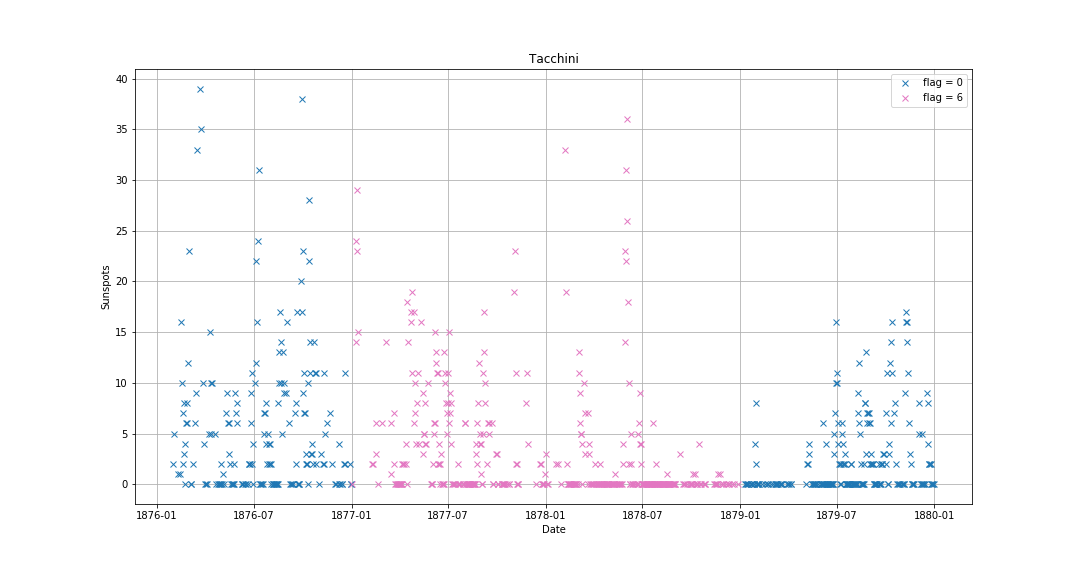
\includegraphics[width=0.5\linewidth]{tacchini1877_patch.png}
    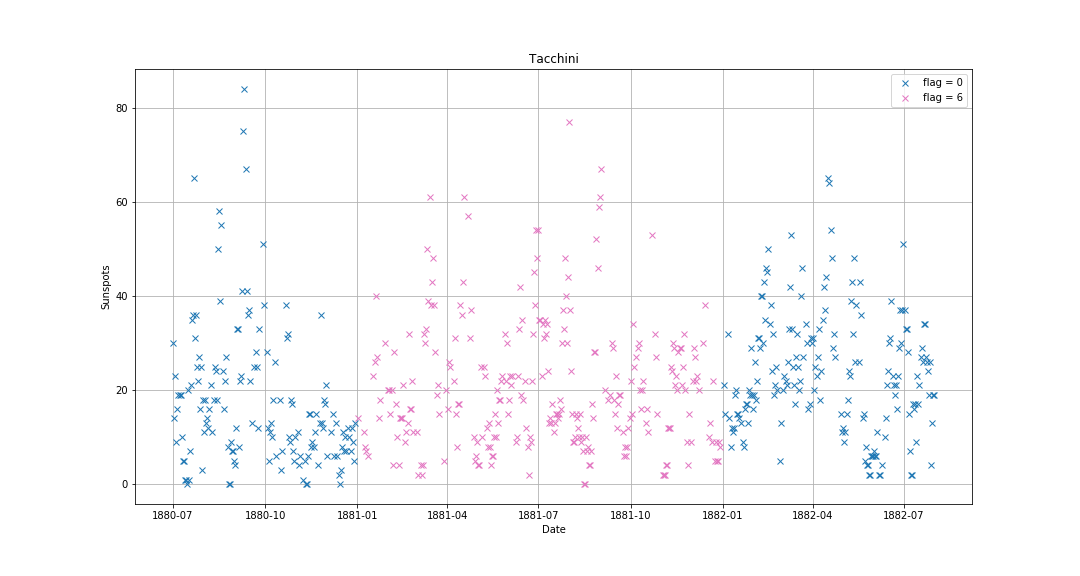
\includegraphics[width=0.5\linewidth]{tacchini1881_patch.png}
    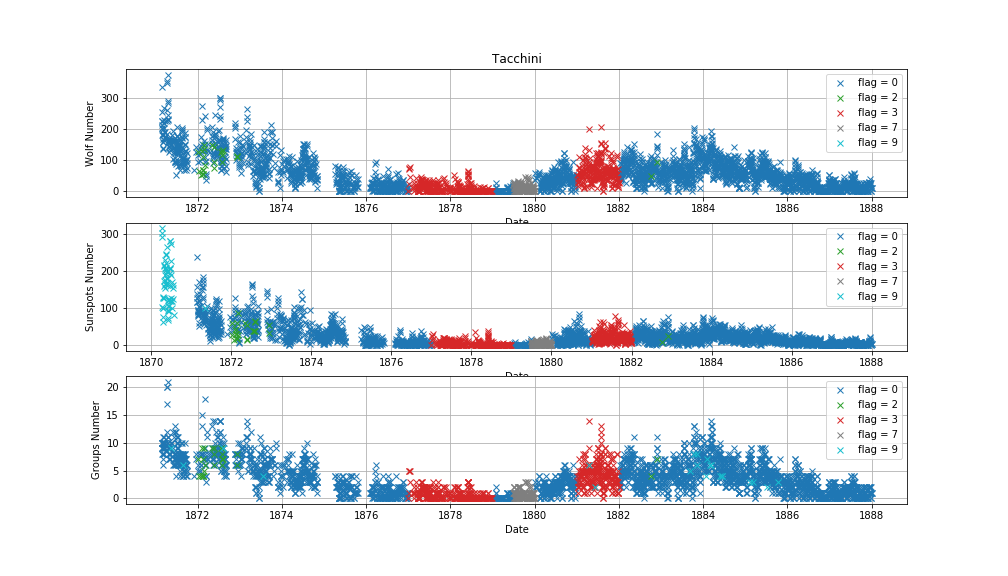
\includegraphics[width=\linewidth]{tacchini_pached.png}
    \caption{Tacchini}
    \label{fig:tacchini}
\end{figure}

\begin{figure}[H]
  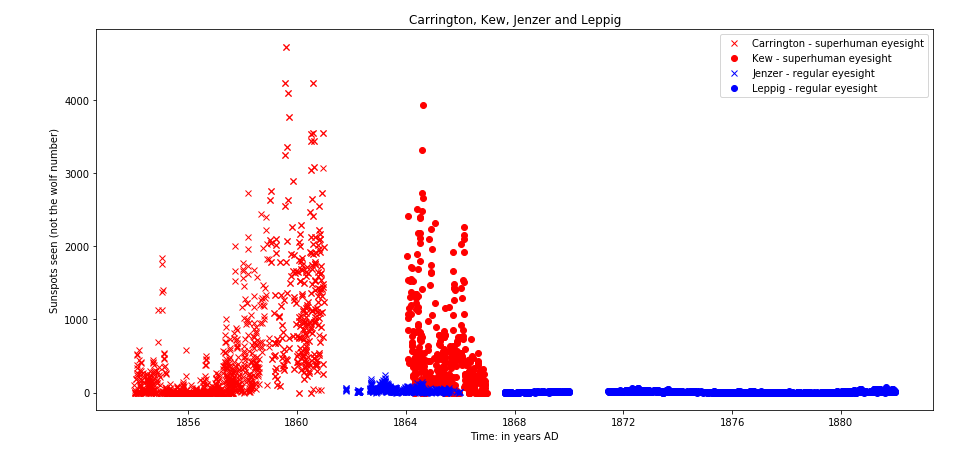
\includegraphics[width=\linewidth]{CarringtonHasGoodEyesight.png}
  \caption{Carrington and Kew - input penumbras instead of sunspots}
  \label{fig:carrington-kew-penumbras}
\end{figure}

\begin{figure}[H]
    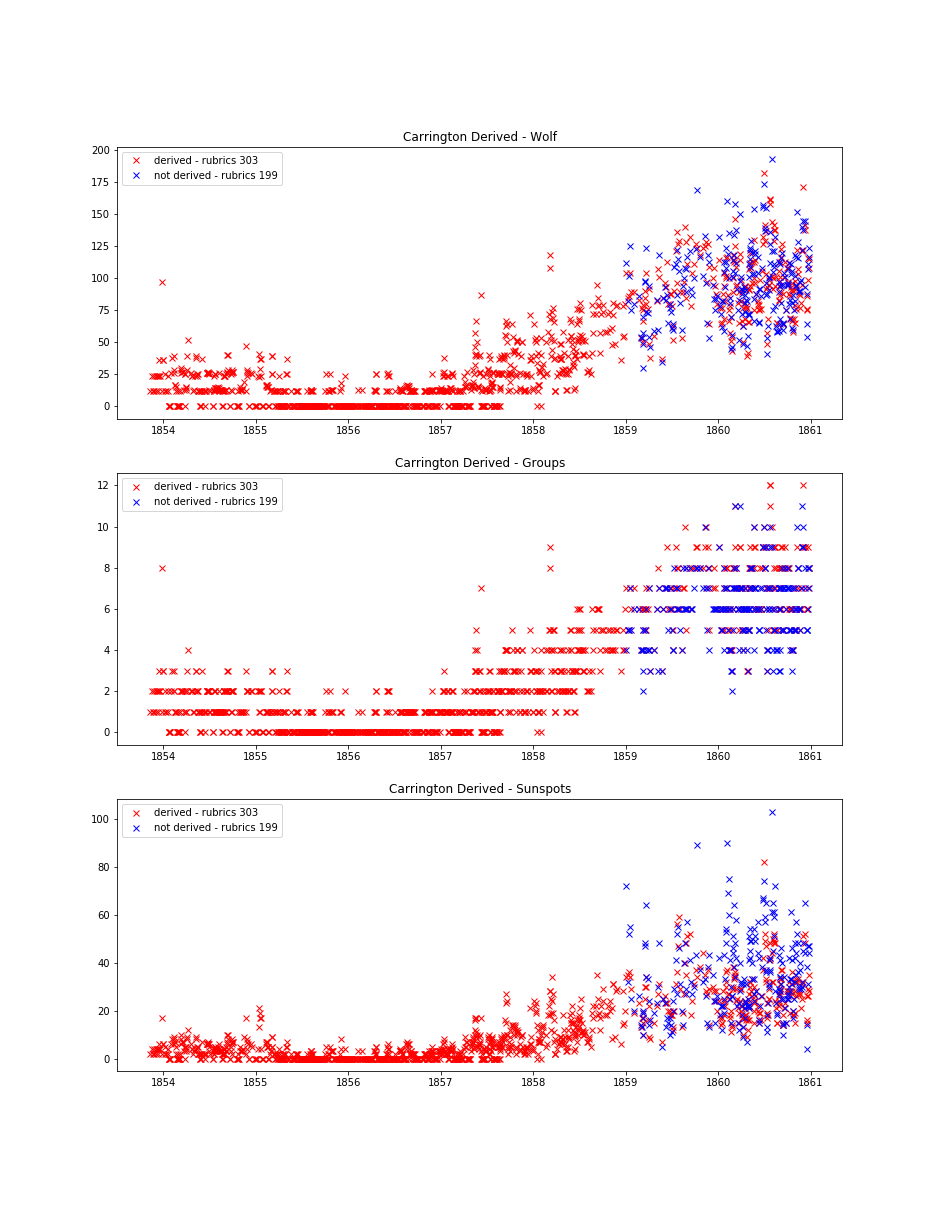
\includegraphics[width=\linewidth]{carrington_derived.png}
    \caption{Carrington derived}
    \label{fig:carrington_derived}
\end{figure}

\begin{figure}[H]
    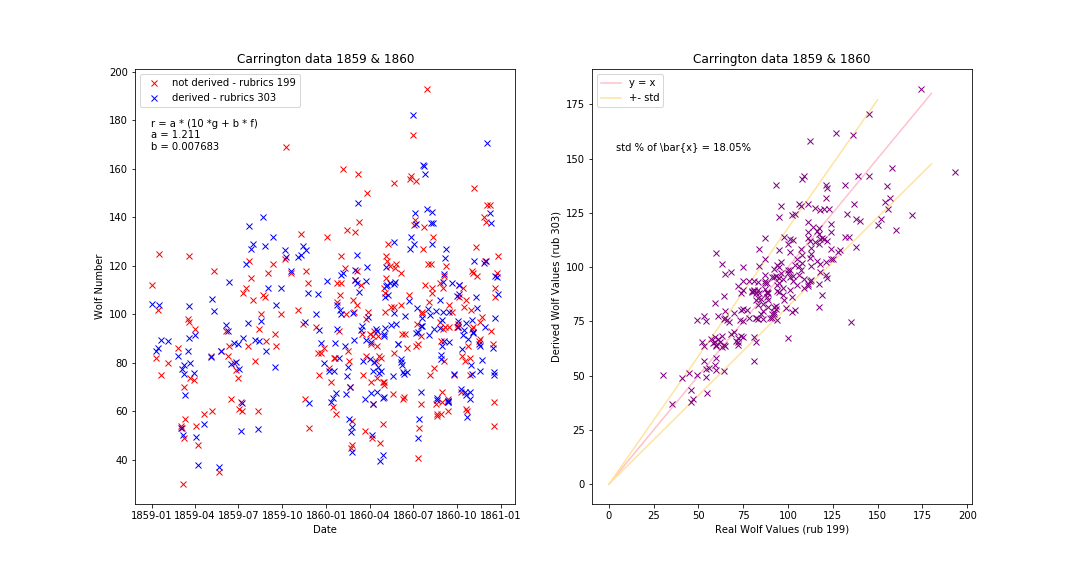
\includegraphics[width=\linewidth]{carrington_fit_wolf.png}
    \caption{Carrington wolf fit}
    \label{fig:carrington_fit_wolf}
\end{figure}

\begin{figure}[H]
    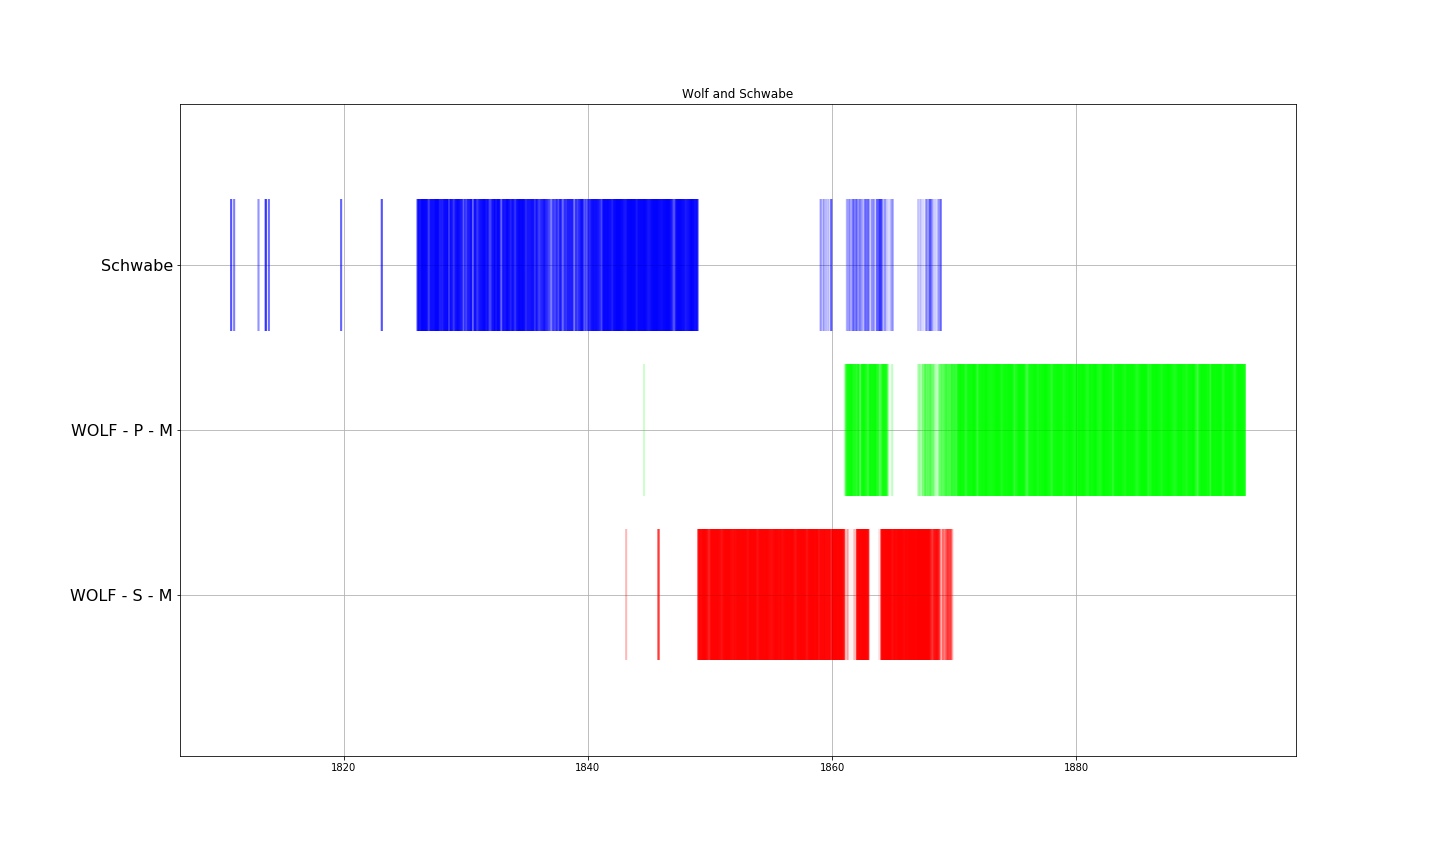
\includegraphics[width=0.5\linewidth]{wolf_and_schwabe_eventplot.png}
    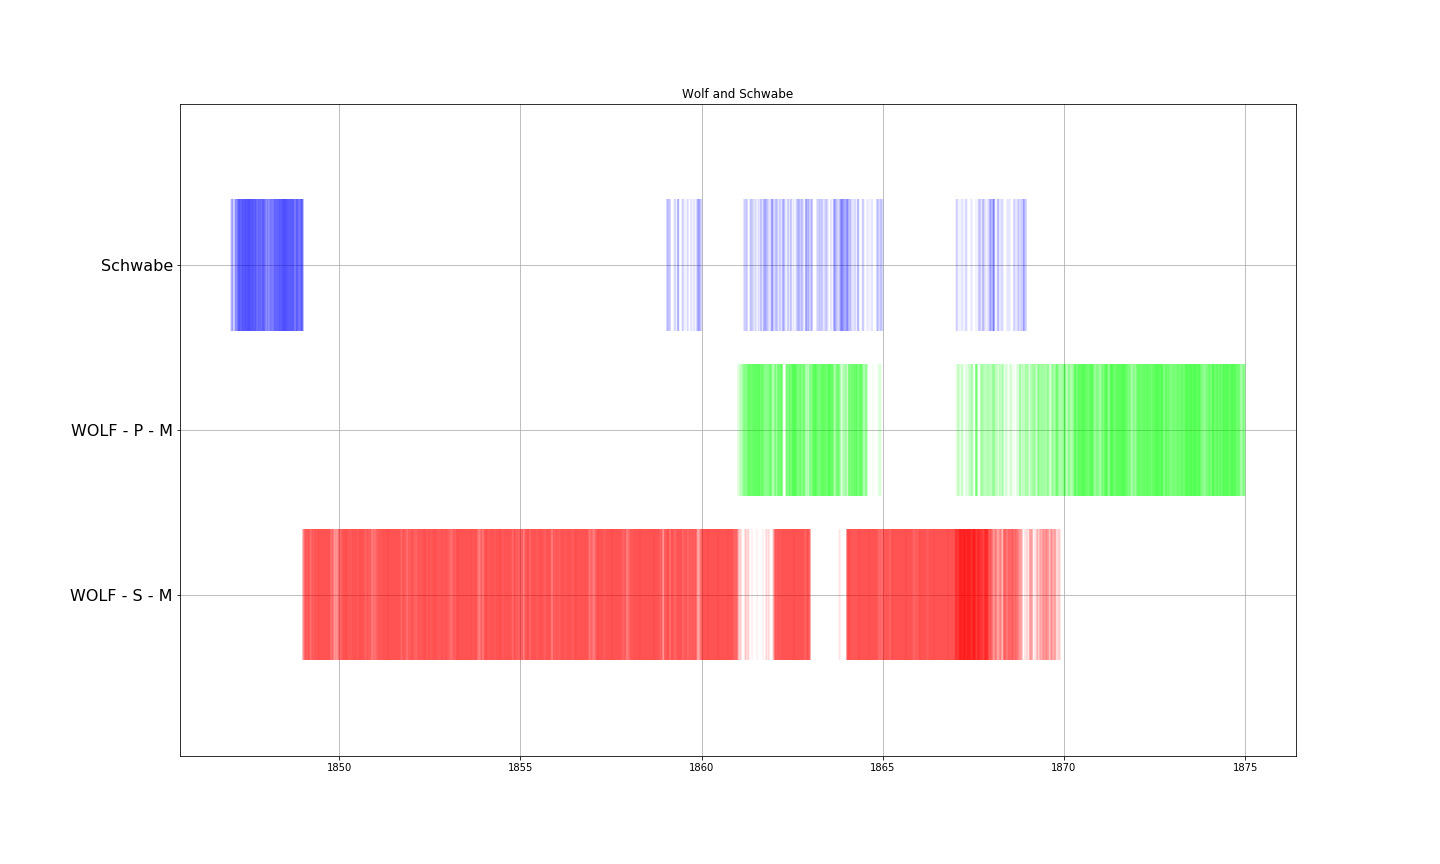
\includegraphics[width=0.5\linewidth]{wolf_and_schwabe_eventplot_1847_1875.png}
    \caption{Wolf and Schwabe Eventplots mon 2019-07-29}
    \label{fig:wolf and schwabe eventplots}
\end{figure}

\begin{figure}[H]
    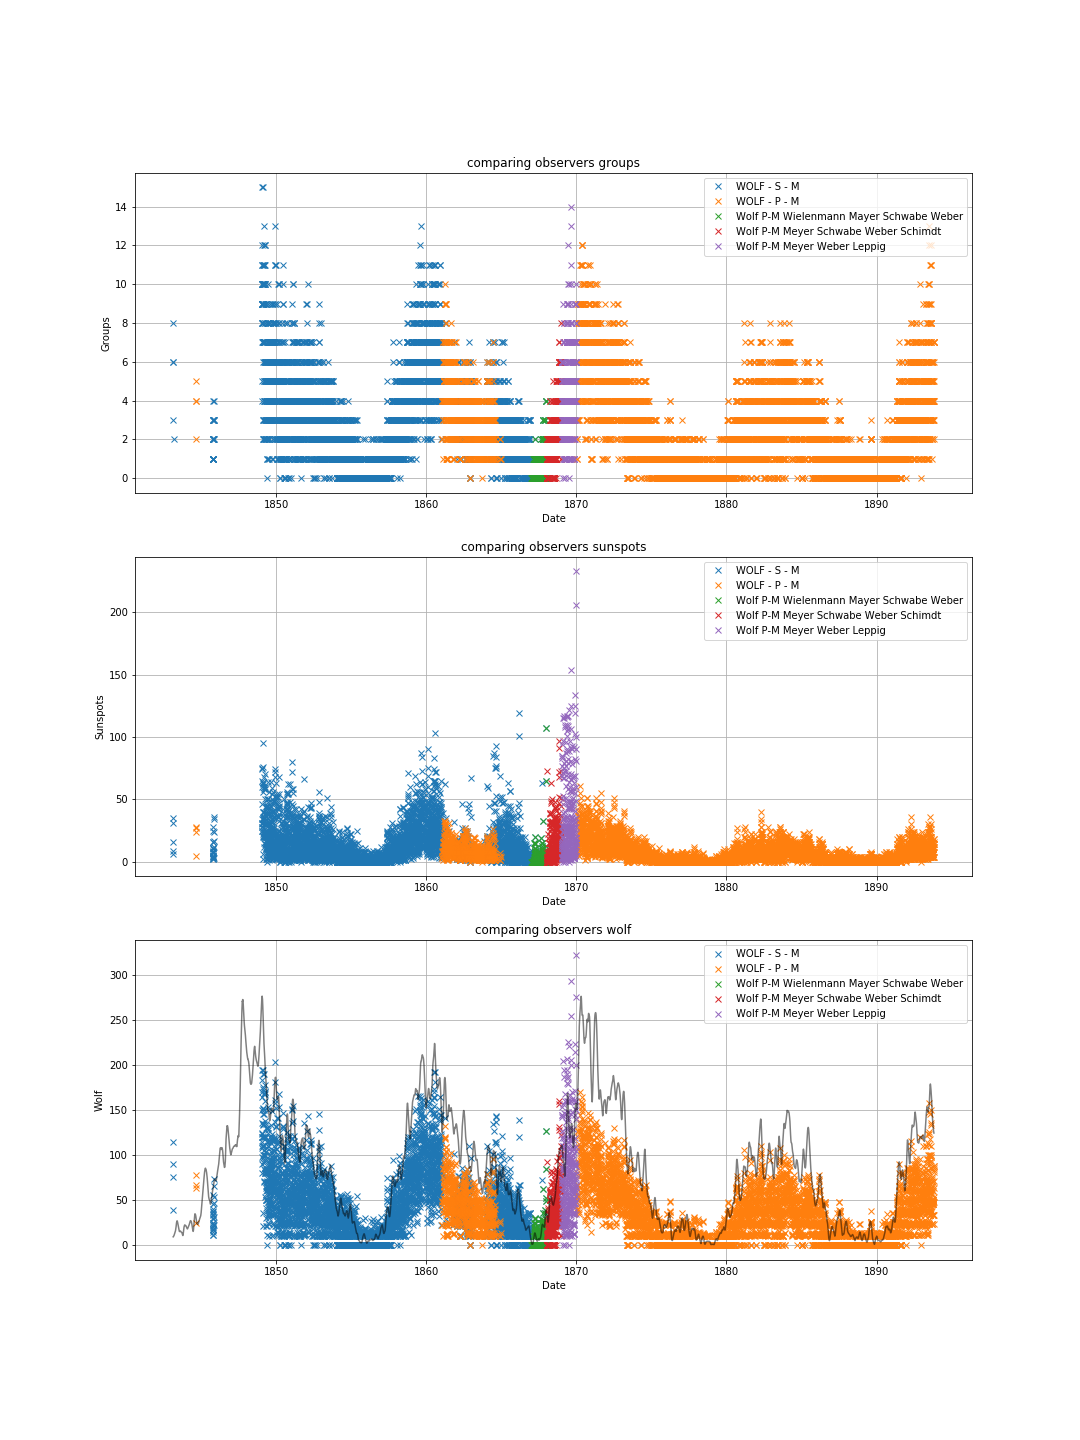
\includegraphics[width=0.5\linewidth]{wolf_comparisons.png}
    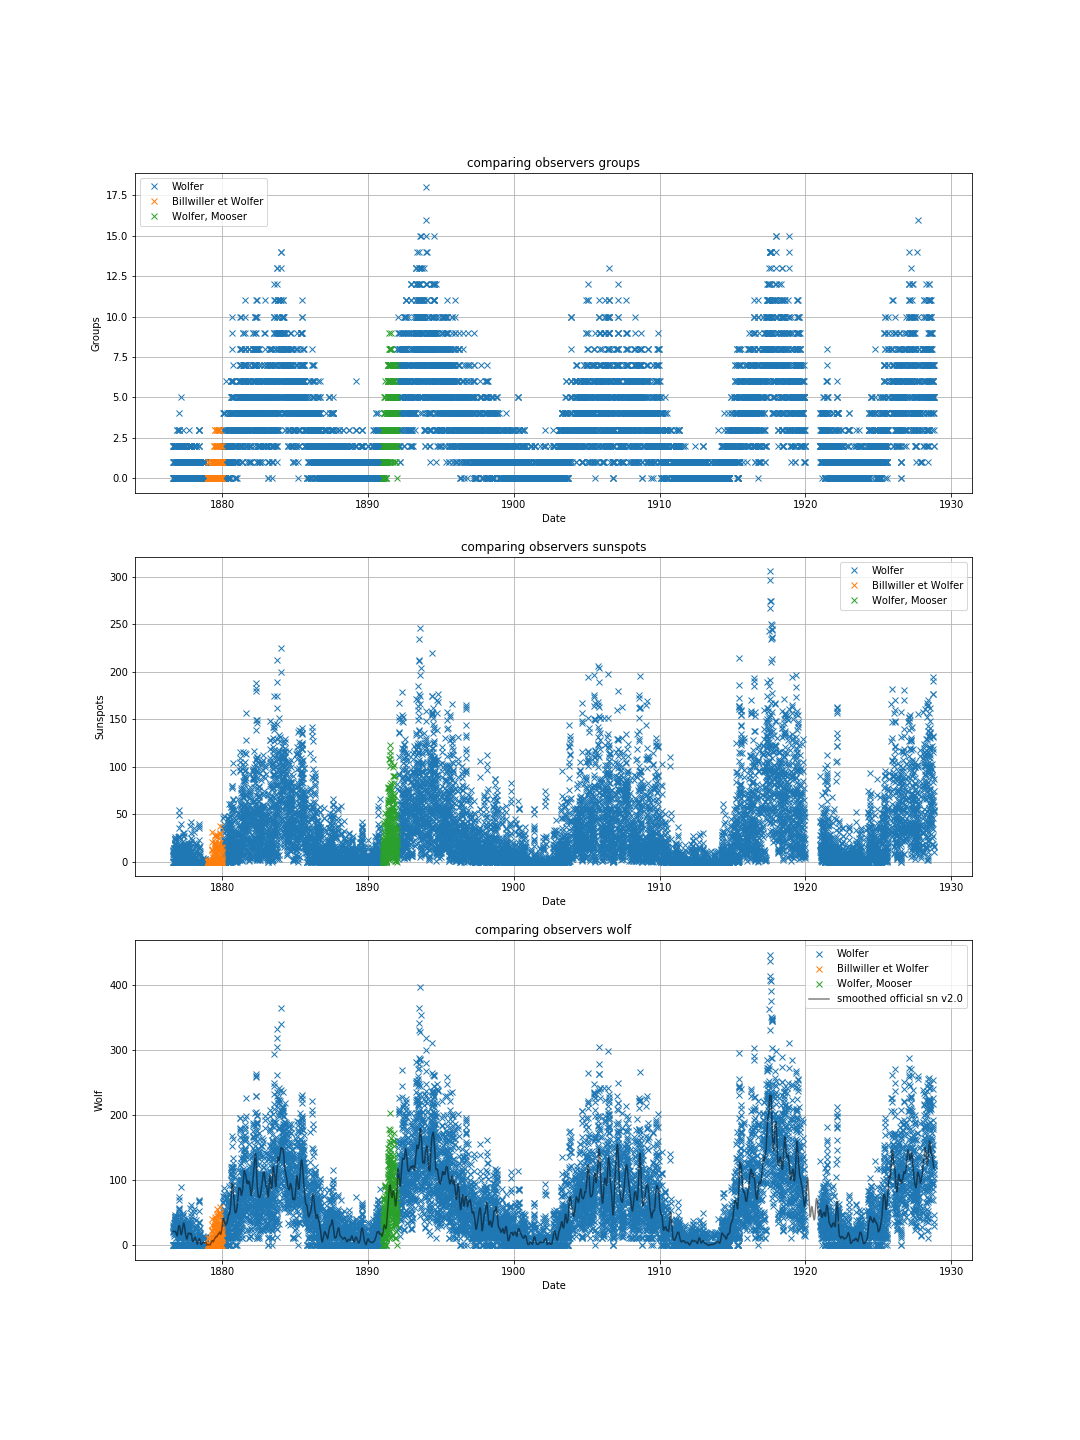
\includegraphics[width=0.5\linewidth]{wolfer_comparisons.png}
    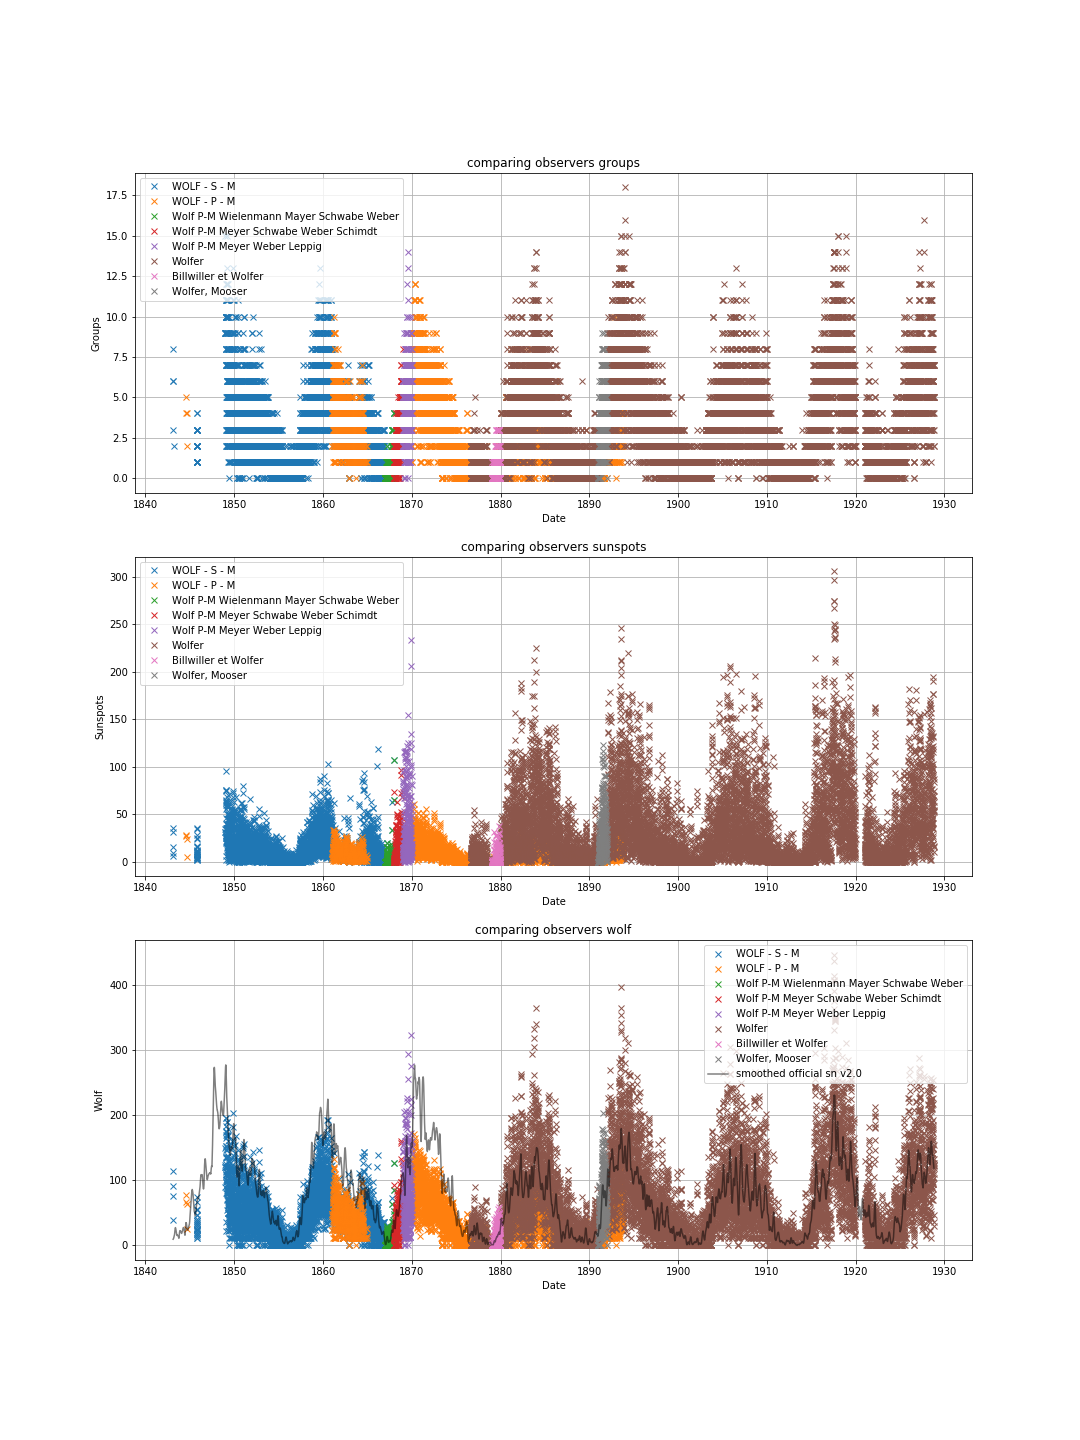
\includegraphics[width=0.5\linewidth]{wolf_and_wolfer_comparisons.png}
    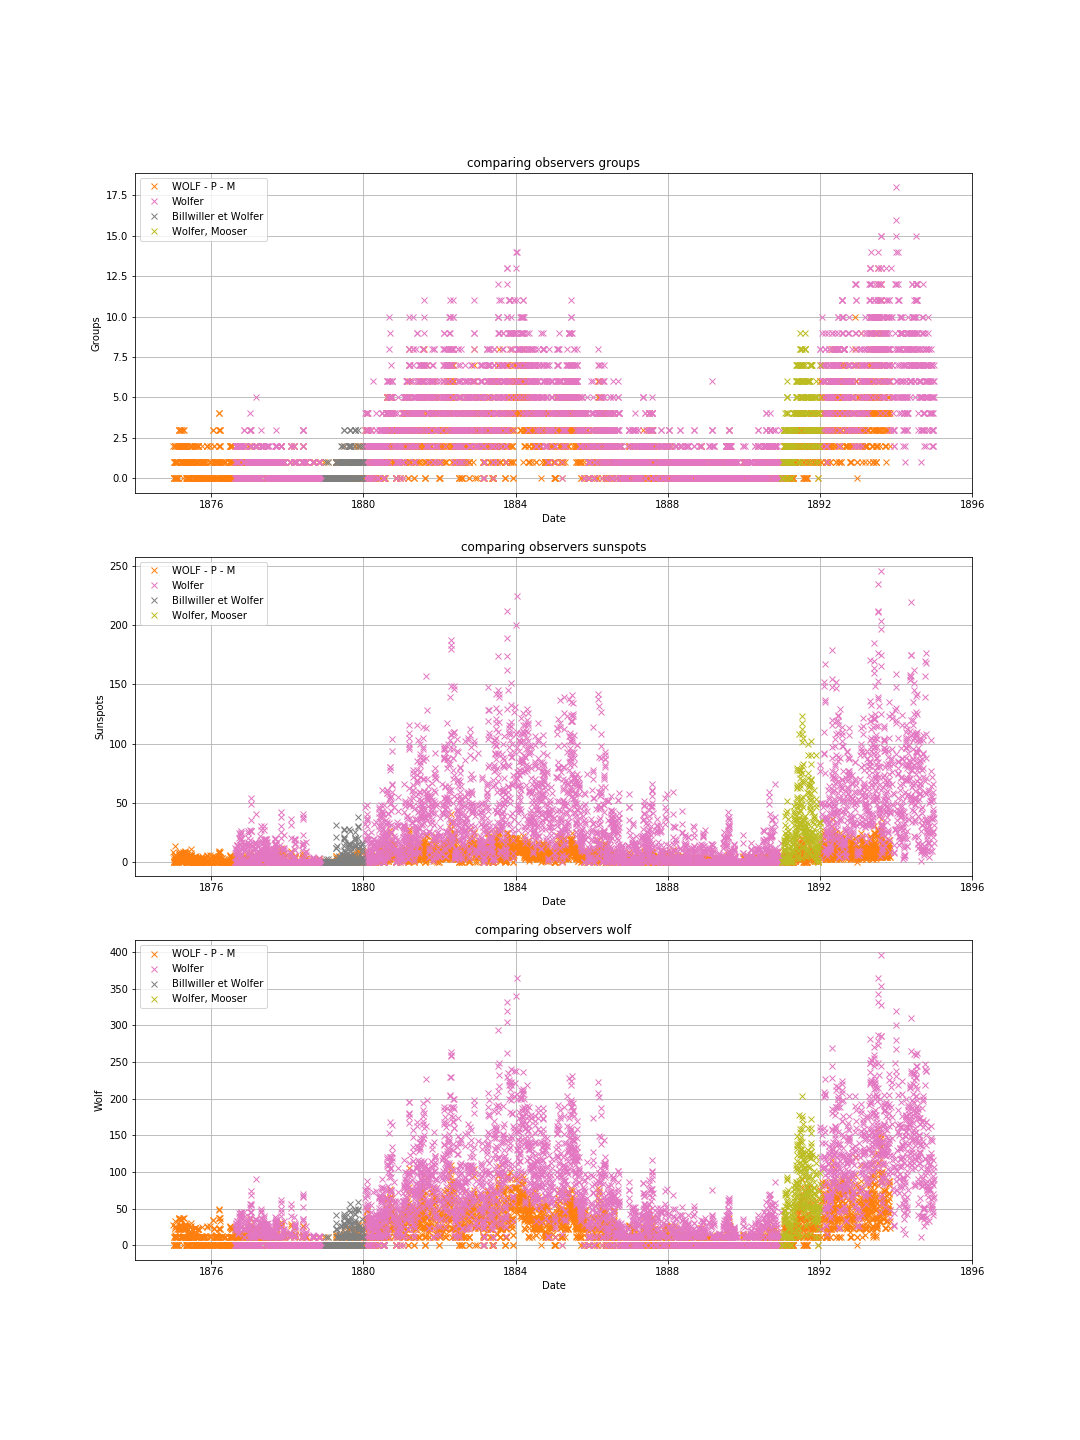
\includegraphics[width=0.5\linewidth]{wolf_and_wolfer_overlap.png}
    \caption{tl = wolf ; tr = wolfer ; bl = wolf and wolfer ; br overlap}
    \label{fig:wolf and wolfer initial plots}
\end{figure}\\


\newpage

\section{Important Rubrics Translated}\label{converting the `aire'}

\subsection{Rubrics 299, Mitt 33, p 128 - Secchi}\label{rubrics 299, secchi}\\

\textbf{German}
p128) Als Anhang ist ein ``[It] Registro della macchie solarie osservate alla specola del Collegio Romano durante l'anno 1871" gegeben, welches die an einer Reihe von Tagen von Rom. Remiddi gezahlten Gruppen, anstatt der Anzahlder Flecken aber Zahlen enthalt, welche die von ihnen eingenomene Flache in Quadrat-Millimeter geben, die Flache der Sonnenscheibe zu 46352,5 Quadrat-Millimeter angenommen. Ich gebe dieselben in der gewohnten Weise, d. h so, dass die erste Zahl wie immer der Anzahl der Gruppen, die zweite aber jener Flachenzahl entspricht, - die der letztern gleichgesetzte Zahl endlish eine aus ihr nach untenstehender Formel berechnete, der Fleckenzahl moglichst entsprechende Zahl.\\

\textit{Secchi's Data from rubrics 299}\\

p 130) Meine Relativzahlen basiren bekanntlich auf der Annahme, dass die Fleckenthatigkeit zunachst in der Anzahl der Gruppen, in untergeordneter Weise aber auch in der Grosse derselben ein Maass finde, und es wurde dieser Grosse von mir nur darum die Gesammtanzahl der Flecken substituirt, weil ich einerseits durch viele betreffend Vergleichungen gefunden hatte, das mit der Grosse der Hauptflecken meistens auch die Anzahl ihre Begleiter zunehem, also die Anzahl der Flecken annahernd jener Grosse proportional sei, - und es anderseits nicht nur zu zeitraubend fand diese Grosse fortwahrend zu messen, und (was bei den obigen Beobachtungen, welche nur die scheinbaren Flachen geben, wenigstens vorlaufig unterlassen wurde) auf ihr wahres Mass zu reduciren, sondern namentlich auch ein fur altere Beobachtungsreihen (denen sich gewohnlich die Anzahl der Flecken mit ziemlicher Sicherheit, die Grosse dagegen selten auch nur irgendwie annahernd entnehmen lasst) ebenfalls brauchbares Verfahren einfuhren musste. - Die in der obigen Reihe fur viele Tage, and welchen ich selbst Fleckenzahlungen gemacht, und daraus die Relativzahlen $r$ berechnet hatte, gegebenen Flachen haben mir nun die Moglichkeit verschafft die Richtigkeit meines Verfahrens neuerdings zu prufen, und zugleich eine bestimmte Regel aufzustellen, um zur Erganzung meiner Register fur einzeln Tage ause den bestimmten Flachen die fur mich nothigen Fleckenzahlen annahernd zu berchnen: Bezeichne ich namlich die Anzahl der in Rom gezahlten Gruppen mit $g$, die bestimmte Flache aber mit $f$, so muss unter Voraussetzung der Richtigkeit meiner Annahme annahernd fur jeden gemeinschaftlichen Beobachtungstag eine Gleichung
$$r = a\cdot (10 g + b \cdot f) = 10 a \cdot g + c \cdot f$$
bestehen, wo a, b und c constante Factoren sind. Ich bildete nun 120 solcher Gleichungen, ordnete dieselben nach r, nahm je aus 20 das Mittel, und erhielt so die 6 Normalgleichungen \\

{\centering
    \begin{tabular}{c|c|c|c}
    
         & $r = 10 a \cdot g + c\codt f$ & $r'$ & $r - r'$ \\
         \hline
         1 & $60 = a \cdot 37 + c \cdot 46$ & $62$ & $-2$ \\
         2 & $80 = a\cdot 46 + c\cdot 61$ & $78$ & $+2$ \\
         3 & $100 = a\cdot 60 + c\cdot 112$ & $109$ & $-9$ \\
         4 & $120 = a\cdot 63 + c\cdot 117$ & $114$ & $+6$ \\
         5 & $140 = a\cdot 78 + c\cdot 155$ & $143$ & $-3$ \\
         6 & $160 = a\cdot 85 + c\cdot 187$ & $159$ & $+1$ \\
         \hline
         & Mittlere Abweichung && \pm{5}
    \end{tabular}
\par}
aus welchen ich nach der Methode der kleinsten Quadrate 
$$a=1.41 \quad c=0.21 \quad \text{sodann}\ b=0.15$$
und somit fur die romischen Beobachtungen die Reductionsgleichung
$$r' = 1.41(g\cdot 10 + f\codt 0.15)$$
fand. Setze man in die Normalgleichungen diese Werthe fur a und c ein, so erhalt man die ihnen beigeschriebenen r', deren Vergleichung mit den r eine unerwartet gute Uebereinstimmung zeigt. Es hat also diese kleine Untersuchung die Berechtigung des von mir fur die Berechnung der Relativzahlen aufgestellten Principes in schonster Weise bestatigt, und mich anderseits ermuthigt in der obigen Beobachtungsreihe jeder Flache die nach der eben aufgefuhrten Formel berechnete Fleckenzahl beizuschreiben, - wobei ich naturlich in den paar Fallen, wo eine ganz geringe Flache eine Fleckenzahl ergab, welche kleiner als die Gruppenzahl war fur sie diese Gruppenzahl substituirte.\\

\textbf{English}
p128) As an appendix is given a ``[It] Register of sunspots observed in the mirror of the Roman College during the year 1871" Collegio Romano durante l'anno 1871", which was held on a series of days of Rome. Remiddi paid groups, instead of the number of spots but contains numbers which give the area in square millimeters inscribed by them, the area of the solar disk is assumed to 46352.5 square millimeters. I give them in the usual way, i.e. in such a way that the first number corresponds, as always, to the number of groups, the second, however, to that number of flats, - which endlessly calculates from the latter equated number a number which corresponds as closely as possible to the number of spots, according to the formula below.\\

\textit{Secchi's Data from rubrics 299}\\

p 130) As is well known, my relative numbers are based on the assumption that the number of spots finds a measure first of all in the number of groups, but in a subordinate way also in the size of the same, and this size was only substituted by me for the total number of spots, because on the one hand I had found by many comparisons that with the size of the main spots mostly also the number of their companions increases, so the number of spots is approximately proportional to that size, - and on the other hand not only too time-consuming was it found to measure these large ones continuously, and (what was at least temporarily omitted in the above observations, which only give the apparent flat ones) to reduce them to their true measure, but especially also to introduce a procedure useful for older series of observations (from which usually the number of spots is quite certain, but the large ones, on the other hand, can seldom be taken out even approximatively) likewise. - The surfaces given in the above series for many days, on which I had made spot payments myself, and had calculated the relative numbers $r$ from them, have now given me the possibility to check the correctness of my method recently, and at the same time to establish a certain rule in order to approximate the numbers of spots necessary for me to supplement my registers for individual days from the certain surfaces: If, for example, I designate the number of groups paid in Rome with $g$, but the certain area with $f$, then, assuming my assumption is correct, an approximate equation must be given for each common observation day
$$r = a\cdot (10 g + b \cdot f) = 10 a \cdot g + c \cdot f$$
where a, b and c are constant factors. I now formed 120 such equations, arranged them according to r, took the mean from each 20, and thus obtained the 6 normal equations \\

{\centering
    \begin{tabular}{c|c|c|c}
    
         & $r = 10 a \cdot g + c\cdot f$ & $r'$ & $r - r'$ \\
         \hline
         1 & $60 = a \cdot 37 + c \cdot 46$ & $62$ & $-2$ \\
         2 & $80 = a\cdot 46 + c\cdot 61$ & $78$ & $+2$ \\
         3 & $100 = a\cdot 60 + c\cdot 112$ & $109$ & $-9$ \\
         4 & $120 = a\cdot 63 + c\cdot 117$ & $114$ & $+6$ \\
         5 & $140 = a\cdot 78 + c\cdot 155$ & $143$ & $-3$ \\
         6 & $160 = a\cdot 85 + c\cdot 187$ & $159$ & $+1$ \\
         \hline
         & Mittlere Abweichung && \pm{5}
    \end{tabular}
\par}

from which I can draw the least squares 
$$a=1.41 \quad c=0.21 \quad \text{sodann}\ b=0.15$$
and therefore for the Roman observations the reduction equation
$$r' = 1.41(g\cdot 10 + f\codt 0.15)$$
found. If one enters this value for a and c in the normal equations, one obtains the r' attributed to them, whose comparison with the r shows an unexpectedly good agreement. So this small examination confirmed in the best way the validity of the principle I had established for the calculation of the relative numbers, and on the other hand it encouraged me in the above series of observations to attribute to each surface the number of spots calculated according to the just listed formula, - whereby I naturally substituted this group number in the few cases where a very small surface resulted in a number of spots which was smaller than the group number for it.

\subsection{Rubrics 303, mitt 35, p 241 observer Carrington}\label{rubrics 303, carrington}\\

303) Warren De La Rue, Balfour Stewart and Benjamin Loewy, Researches on Solar Physics. Second Series: Area measurements of the Sun-Spots observed by Carrington during the seven Years from 1854 - 1860 inclusive, and deductions therefrom. London 1866 in 4.\\

\textbf{German}
Ich ziehe aus dieser Abhandlung unter fortwahrender Berucksichtigung der unter 199 besprochenen Werkes von Carrington und der unter 129 aufgeguhrten schriftlichen Mittheilung derselben folgende Beobachtungen in der altgebohnten Form, nur dass die der Gruppenzahl folgende Zahl (analog wie bei den unter 299 aufgeguhrten Beobachtungen Secchis) nicht die Anzahl der Flecken, sondern die in Millionsteln der sichtbaren Sonnenhemisphare ausgedruckte Flache derselben Bezeichnen:\\

Durch Vergleichung der fur 1859 und 1860 gegebenen Flachenzahlen mit den in Nr. 199 von Carrington selbst fur dieselben Jahre und Tage mir mitgetheilten Fleckenzahlen, erhalt man, dass durchschnittlich 1000 Flacheneinheiten 24 Flecken entsprechen, und es darf dieses Verhaltniss ohne Anstand benutzt werden, um fur die wenigen Tage, wo das Fleckenregister durch Carrington'sche Beobachtungen erganzt werden kan, die Flachen in Flecken umzusetzen.\\

\textbf{English}
I deduce from this treatise, taking into account the work of Carrington discussed under 199 and the written communication of the same discussed under 129, the following observations in the old-bored form, only that the number following the group number (analogous as in the observations of Secchi examined under 299) does not denote the number of spots, but the area of the same printed out in millionths of the visible solar hemispheres:\\

What follows is observations made by Carrington for the years specified with `aire' numbers instead of sunspots numbers. [it seems someone had the same idea as me]\\

By comparing the surface numbers given for 1859 and 1860 with the spot numbers given in No. 199 by Carrington himself for the same years and days, one obtains that on average 1000 surface units correspond to 24 spots, and this relationship may be used without decency to convert the surfaces into spots for the few days when the spot register can be supplemented by Carrington's observations.

\subsection{Rubrics 199, mitt 11-20, p224 - Carrington}\label{mitt:rubrics 199}

Observations of the Spots on the Sun from 1853 XI 9 to 1861 III 24 made ad Redhill by R. Chr. Carrington. London 1863 (248 Pag., 166 Plat.) in 4.\\

\textbf{German} 
Dieses Ausgezeichnete, erst kurzlich nach Verdienen von der Pariser-Academie mit dem Lalande-Preise bedachte Werk meines verehrten Freundes erlaubt nach seiner Natur kaum einen Auszug, sondern ist zunachst als eine unerschopfliche Fundgrube zu betrachten, in der diejenigen Astronomen, welche sich speqiell mit der Vertheilung der Sonnenflecken, ihren Ortsveranderungen etc. Befassen, ein reiches Material an Zahlen unde Zeichnungen erheben konnen, - wie ja bereits oben eine darauf gegrundete Studie von Herrn Fritz mitgetheilt worden ist, wahrend eine die `Concluding Section' betreffende Arbeit von mir in einer der nachsten Mittheilungen folgen wird. Dagegen mogen hier anhangsweise zur Erganzung der Nr. 129 der Litteratur die Fleckenzahlungen in den Jahren 1859 und 1860 nachgetragen werden, welche mir Herr Carrington seiner Zeit mittheilte, und die ich in der letzten Zeit neuerdings bei Ermittlung der mehrfach erwahnten 5 taggigen Mittel benutzte. Es sind Folgende:\\

\textbf{English}
This excellent work of my esteemed friend, which was awarded the Lalande Prize by the Paris Academy only shortly after it had been earned, hardly permits an excerpt by its nature, but is first to be regarded as an inexhaustible treasure trove in which those astronomers who are particularly concerned with the distribution of sunspots, their changes of place, etc., can be found. As already above a study based on it has been shared by Mr. Fritz, while a work of mine concerning the 'Concluding Section' will follow in one of the next communications. On the other hand, to supplement the No. 129 of the Litteratur, the stain payments in the years 1859 and 1860, which Mr. Carrington informed me of his time and which I recently used in the determination of the repeatedly mentioned 5-day means, may be added here as an appendix. They are the following:

\subsection{Rubrics 375, mitt 41-50, p244 - Secchi}\label{rubrics 375}

\textbf{German}
Herr Professor Secchi in Rom und sein Adjunkt Ferrari haben 1877 folgende Gruppen-Zahlungen und Flachenbestimmungen erhalten, und theils in ihrem Vulletino theils in gefalligster Weise direct mitgetheilt:\\

Die zweiten der hier gegebenen Zahlen geben nicht, wie bei den ubringen Serien, die Anzahl der Flecken, sondern sind der Rubrik 'Area mm quadrati' entommen in welcher eine Einheit 21.56 Millionstel der Flache der Sonnenscheibe entsprechen soll\\

\textbf{English}
In 1877 Professor Secchi in Rome and his adjunct Ferrari received the following group payments and area determinations, and some of them in their Vulletino in the most pleasing way directly informed:\\

The second of the numbers given here do not give, as in the ubringen series, the number of the spots, but are taken from the column 'Area mm quadrati' in which one unit should correspond to 21.56 millionths of the area of the solar disk.\\

\subsection{Rubrics 293, mitt 31-40, p114 - Johann Friedrich Julius Schmidt}\label{rubrics 293}

\textbf{German}
Sonnenfleckenbeobachtungen in Athen im Jahre 1872. Aus einem Schreiben von Jul. Schmidt, datirt: Athen 1873 I 2.
Herr Director Jul. Schmidt hat im Jahre 1872 folgende Fleckenzahlungen erhalten:\\

durch Herrn Prof. Heis in Munster auf meine Bitte vor dem Abdrucke im Mss. mitgetheilt.\\

*) Die Beobachtungen von Augus bis Ende Jahres wurden mir ducrch Herrn Professor Heis auf meine Bitte vor dem Abdrucke im Mss. mitgetheilt. \\

Die vollstandigen Beobachtungen sind mit dem sechsfussigen Refractor der Athener-Sternwarte gemacht, - die ubringen mit einem zweifussigen. Wie schade, dass versaumt wurde auch mit dem kleinern Instrumente die Fleckenzahlungen auszufuhren, und so diese, namentlich fur die Wintermonate an Beobachtungstagen so reiche Serie, ohne viel grossere Muhe noch viel brauchbarer und werthvoller zu machen, als sie dadurch werden, dass man die AthenerGruppenzahlen g nach folgender aus vielen Vergleichungen festgestellten mittlern Scale in Relativzahlen r umsetze. Es entsprechen sich namlish im Mittel

wovon ich fur die wenigen Tage, welche ich in meiner JahresTabelle fur 1872 noch auszufullen hatte, wirklich Gebrauch machte\\

{\centering
    \caption{Conversion table from rubrics 293}
    \begin{tabular}{c|c c c c c c c c c c c c c c }
        $g$ & 0 & 1 & 2 & 3 & 4 & 5 & 6 & 7 & 8 & 9 & 10 & 11 & 12 & 13 \\
        \hline
        $r$ & 0 & 20 & 38 & 54 & 69 & 83 & 97 & 110 & 123 & 136 & 148 & 160 & 172 & 184
    \end{tabular}
    
    \label{table:silly table version 2}
\par}\\

\\ 

\textbf{English}
Sunspot observations in Athens in 1872. From a letter by Jul. Schmidt, dated: Athens 1873 I 2.
Mr. Director Jul. Schmidt received the following spot numbers in 1872:

by Prof. Heis in Munster at my request before the impression in mass.

*) The observations from August to the end of the year were sent to me by Professor Heis at my request before the impression in Mass. 

The complete observations are made with the six-foot refractor of the Athens Observatory, - the ones with a two-foot refractor. What a pity that it was neglected also with the smaller instruments to carry out the spot payments, and so this series so rich, especially for the winter months on observation days, without making much greater effort still much more useful and valuable than they become by converting the Athenian group numbers g according to the following mean scale determined from many comparisons in relative numbers r. The following correspond namlishly on average

which I really made use of for the few days which I still had to fill out in my year table for 1872.

\subsection{Mitt 24 page 103}\label{mitt:mitt 24 page 103}

\textbf{German}
XXIV. Beobachtungen der Sonnenflecken im Jahre 1867 und Berechnung der Relativzahlen und Variationen dieses Jahres; vorlaufige Bestimmung der Epoch des letzten Minimums, Zusammenstellung der bisherigen Epochen und Relativzahlen, sowie einige betreffende Schlusse und Rechnungsresultate; uber die behufs Ortsbestimmung der Sternwarte ausgefuhrten und beabsichtigen Operationen, speziell uber die bestimmung der Lange, des Nadirs, der Collimation und Refraction; Fortsetzung der Sonnenfleckenliteratur.\\

Die Haufigkeit der Sonnenflecken konnte von mir oder meinen Assistent, Herrn Weilenman und Meyer, im Lauf des Jahres 1857 an 299 Tagen mehr oder weniger vollstandig beobachtet werden, und ausserdem erhielt ich von den Herrn Hofrath Schwabe in Dessau und Weber in Peckeloh (s. 246 der Litt.) eine ziemlich grosse Anzahl werthvoller Erganzungen, so dass ich schliesslich fur 356 uber vollstandige, zum Theil sogar uber mehrfache Beobachtungen verfugte und nur bei 9 Tagen (2 im Januar und 7 im Dezember) in ganzlicher Unkenntniss uber den Fleckenstand der Sonne bleib. - Wie bei den Berichten uber 1863 bis 1866 habe ich in der ersten der beistehenden Tafelt fur jeden Tag in algewohnter Weise die Anzahl der gesehenen Gruppen und Flecken eingetragen, und bei jeder Beobachtung, mit einziger Ausnahme der entweder von mir selbst oder von den Herrn Weilenmann und Meyer nach ganz entsprechender Arrt mit Vergrosserung 64 meines Vierfussers erhalten Normalbeobachtungen, durch ein beigefugtes Zeichen den Beobachter markirt, um bei Berechnung der Relativzahlen den ihm zugehorigen Reductions-factor anweden zu konnen. Ein beigesetztes \dag bezeichnet beobachtungen meines geehrten Herrn Hofrath Schwabe (mit Reductionsfactors 5/4), der nach seiner neulichen Einsendung in die Monthly Notices of the Royal Astronomical Society (Vol. 28, Nr. 3) im Ganzen in den 12 Monaten von 1867\\

Beobachtungstage: 13 16 16 14 16 30 31 31 30 28 22 15\\
Fleckenfreie Tage:    23 26 15 16 16 23 18 20 17 13 5 3\\
Gruppen:      0   0   3   1    2   1   2    3   1   3 4 5\\

erhielt, also bei 312 Beobachtungstagen die Sonne 195 mal ohne Flecken sah (wahrend die zweite der beistehenden Tafeln auf 356 Tage 199, die erste sogar 216 ohne Flecken hat) und wahrend des ganzen Jahres 25 Gruppen (21 weniger als 1866, und 68 weniger als 1865) zahlte. - Ein beigestztes * bezeichnet Beobachtungen, welche ich (vergl. Nr. XII) mit dem kleinen Instrumente machte und mit 3/2 in Rechnung brachte. - Mit Hulfe dieser Beobachtungen und Reductionsfactoren wurden nun fur die erwahnten 356 Tage die Relativzahlen berechnet, und daraus theils die in die Tafel eingetragenen Monatsmittel, theils als mittlere Relativzahl des Jahres 1867 gefunden. - Die zwite der beistehenden Tafeln gibt fur jeden derselben 356 Tage die ihm zukommende Relativzahl, - jedoch (entsprechend den Berichten seit 1863) mit dem Unterschiede, dass letztere sich nicht allein auf die in ersterer Tafel eingetragene Beobachtung grundet, sondern dass fur sie ausser der Wolf-Schwabe'schen Serie sammtliche 306 Weber'schen Beobachtungen benutzt wurden, welche in Nr. 246 der Literatur verzeichnet sind. Ferner gibt die zweite Tafel die funftagigen Mittel dieser mittlern taglichen Relativzahlen, so wie fur jeden Monat das Mittel der 6 (oder im August 7) auf ihn fallenden funftagigen Mittelzahlen. Diese 12 letztern Zahlen stimmen naturlich mit den Monatsmitteln der esten Tafel nicht ganz uberein, und so ist auch das aus ihnen gezogene Jahresmittel\\

R' = 8,3\\

etwas von dem aus der ersten Tafel erhalten Werthe R versichieden. Mit Zugrundelegung dieser Werthe erhalte ich nach den von mir aufgestellten Formeln, folgende magnetische Declinationsvariationen :\\

\<tafel\>
\hdots \text{continues ad inf}\\


\textbf{English}
XXIV. observations of the sunspots in 1867 and calculation of the relative numbers and variations of this year; preliminary determination of the epoch of the last minimum, compilation of the previous epochs and relative numbers, as well as some concerning conclusions and calculation results; about the determination of the position of the observatory carried out and intended operations, especially about the determination of the longitude, the nadir, the collimation and refraction; continuation of the sunspot literature.\\

The frequency of the sunspots could be observed more or less completely by me or my assistant, Mr. Weilenman and Meyer, in the course of the year 1857 on 299 days, and in addition I received from Mr. Hofrath Schwabe in Dessau and Weber in Peckeloh (see 246 of the Litt.) a quite large number of valuable additions, so that I finally had for 356 complete, in part even multiple observations and remained only at 9 days (2 in January and 7 in December) in complete ignorance of the spot position of the sun. - As in the reports about 1863 to 1866 I have entered the number of the seen groups and spots for each day in the first of the accompanying tables in the usual way, and with each observation, with only exception of the normal observations received either by myself or by Mr. Weilenmann and Mr. Meyer after quite corresponding manner with enlargement 64 of my quadruped, by an attached sign the observer marks, in order to be able to apply the reduction factor belonging to him with calculation of the relative numbers, the reduction factor. A buried \dag denotes observations of my honoured Mr. Hofrath Schwabe (with reduction factor 5/4), who after his recent submission to the Monthly Notices of the Royal Astronomical Society (Vol. 28, No. 3) in the whole in the 12 months of 1867\\

Observation days: 13 16 16 14 16 30 31 31 30 28 22 15\\
Stain-free days: 23 26 15 16 16 23 18 20 17 13 5 3\\
Groups: 0 0 3 1 2 1 2 1 2 3 1 3 4 5\\

so, at 312 days of observation the Sun saw 195 times without spots (while the second of the accompanying tables saw on 356 days 199, the first even has 216 without spots) and paid 25 groups during the whole year (21 less than 1866, and 68 less than 1865). - An enclosed * indicates observations which I made (cf. no. XII) with the small instrument and charged with 3/2. - With the help of these observations and reduction factors the relative numbers for the mentioned 356 days were calculated, and partly the monthly averages entered in the table, partly the mean relative numbers of 1867 were found. - For each of the same 356 days the two of the accompanying tables give the relative number due to him, - however (according to the reports since 1863) with the difference that the latter are not based solely on the observation entered in the first table, but that for them besides Wolf-Schwabe's series all 306 Weber's observations were used, which are listed in no. 246 of the literature. Furthermore, the second table gives the five-day mean of these mean daily relative numbers, as for each month the mean of the 6 (or in August 7) five-day mean falling on it. These last 12 numbers naturally do not quite coincide with the monthly averages of the first table, and so too is the annual average drawn from them. \\

R' = 8,3\\

some of the value preserved from the first table was R versichieden. Using this value as a basis, I get the following magnetic declination variations according to the formulas I have set up:\\

\hdots \text{continues ad inf}


\subsection{Mitt 83 Rubrics 684, pages 97 to 106}\label{mitt:rub 684}

\subsubsection{Pages 97 and 98 $1^{st}$ half}\label{mitt:rub 684 intro}
\textbf{German}
684) Aeltere Sonnenflecken-Beobachtungen auf der Sternwarte in Kremsmunster.\\

Herr Professor Fr. Schwab, adjunkt der Sternwarte in Kremsmunster, schreib mir unter dem 10. August 1893: "In unsert alten Beobachtungsjournalen finden sich zerstreute Notizen uber Sonnenflecken, und zwar aus den Jahren 1802-1830. Es wurde namlich damals die Zeit meist mit Hilfe von sonnenhohen bestimmt, und von den bei dieser Gelegenheit bemerkten Sonnenflecken mitunter eine kleine Skizze angefertigt, - seltener (besonders in den ersten Jahren ) eine Bemerkung beigfugt; genauer und ausfuhrlicher gescheiht diess in den Jahren 1825-1828.\\

Es finden sich Skizzen, die offenbar nur die auffalligsten Flecken enthalten, im Jahre: \\

---small table with dates and values, not the usual type of table---\\

In den letzten Jahren (1825-29) wurde auch der Abstand der Flecken vom Rande gemessen, um daraus die Elemente Wissens nie ausgefuhrt worden is. - Sollten Sie derartige Notizen verwenden konnen, so bin ich gerne bereit, dieselben ubersichtlich zusammenzustellen, nur bitte ich, mir anzugeben, in welcher Weise diess am zweckmassigsten gschehen konnte" 
-Es ist kaum nothig zu bemerken, dass mich die Mittheilung von Herrn Prof. Schwab im hochsten Grade interessirte, dass ich ihm davon sofort Kunde Gab, und sein Anerbieten unter Beifugung der gewunschten Directionen mit grossem Danke annahm. Die Folg davon war, dass mir Herr Prof. Schwab alsobald, unter Beifugung der nothigen Erlauterungen, folgende zwei Serien ubersandte:\\

\textbf{English}
684) Older sunspot observations at the observatory in Kremsmunster.\\

Professor Fr. Schwab, adjunkt of the observatory in Kremsmunster, wrote to me on 10 August 1893: "In our old observation journals you can find scattered notes about sunspots, namely from the years 1802-1830. In those days the time was mostly determined with the help of sun-high ones, and from the sunspots noticed on this occasion sometimes a small sketch was made, - more rarely (especially in the first years) a remark was added; more exactly and more extensively this happened in the years 1825-1828.\\

There are sketches, which obviously contain only the most conspicuous spots, in the year: \\

---small table with dates and values, not the usual type of table---\\

In the last years (1825-29) also the distance of the spots from the edge was measured, so that the elements of knowledge were never carried out. - Should you be able to use such notes, I am willing to put them together clearly, but I would ask you to tell me how this could be done most expediently". 
-It is hardly necessary to notice that I was extremely interested in Prof. Schwab's announcement, that I immediately gave him a client of it, and accepted his offer with a big thank you and the desired directions. The consequence of this was that Prof. Schwab sent me the following two series as soon as possible, accompanied by the necessary explanations:\\

\subsubsection{Part 1 pages 98 $2^{nd}$ half and 99}\label{mitt:rub 684 part 1}
\textbf{German}
I. Beobachtungen aus den Jahren 1802-1824.\\

"Das Instrument, mit welchem bis 1824 in der Regel beobachtet wurde, war ein (schon von Fixlmillner benutzter) Brander'scher Azimutal-Quadrant mit einem Fernrohr von 5 1/2 Fuss Lange. - Da nur in einigen Jahren neben der Skizze Bemerkungen stehen, so glaubte ich der Uebersichtlichkeit und Einfachheit halber die gewohnliche tabellarische Form wohlen zu sollen, jene Jahre ausgenommen, an denen nur an ganz wenigen Tagen Flecken angemerkt sind. (Fur die Publication have ich vorgezogen ausschliesslich die von mir seit Jahren gebrauchte Weise anzuwenden, und in einzelen Fallen nachzuhelfen.) An jenen Tagen, an denen die Sonne beobachtet wurde, ohne dass uber Flecken etwas angemerkt ware, wurde O angesetzt, was gerade nicht heissen muss, dass die Sonne fleckenfrei gewesen, aber doch darauf hinweist, dass dem Beobachter nichts besonderes an der Sonnenoberflache aufgefallen sei ; freilich konnte auch manchmal die Anfertigung der Skizze aus Mangel an Zeit unterlassen worden sein"\\

\textbf{English}
I. Observations from the years 1802-1824.\\

"The instrument with which observations were usually made until 1824 was a Branderian azimuth quadrant (already used by \href{https://de.wikipedia.org/wiki/Alexander_Fixlmillner}{Alexander Fixlmillner} or more likely his nephew \href{https://en.wikipedia.org/wiki/Placidus_Fixlmillner}{Placidus Fixlmillner} (astronomer 1721 to 1791)) with a telescope of 5 1/2 feet long. - Since only in a few years there are remarks next to the sketch, I believed for the sake of clarity and simplicity to use the usual tabular form, with the exception of those years in which spots are noted on only a few days. (For the publication I have preferred to use exclusively the method I have used for years, and to help in individual cases.) On those days when the sun was observed without any notice of stains, 0 was applied, which does not necessarily mean that the sun was spotless, but indicates that the observer had not noticed anything special about the surface of the sun; of course, the sketch could sometimes have been omitted for lack of time".\\

\subsubsection{Part 1 table footnotes}\label{mitt:rub 684 part 1 footnotes}
\textbf{German}
p 100.\\
1) Im November 1805 Kriegsunruhen ; Durchzug der Franzosen. \\

2) Die in die Tagescolumne unter Vorsetzung einse * eingeschriebenen Zahlen geben an, wie oft die Sonne beobachtet wurde, ohne dass etwas von Flecken gesagt oder eine Skizze entworfen worden ist: So Z. B. bezeichnet 1806 I*1, dass die Sonne im Januar dieses Jahres einmal, - II *2 dass sie ausser II 27 im Februar noch an zwei Tagen beobachtet wurde, - u.s.f.\\

3) Die Sonne wurde 1807 behufs der Zeitbestimmung, ausser den 8, noch an 88 Tagen beobachtet; doch ist an denselben uber Sonnenflecken nichts angemerks.\\

p 101.\\
101. 
1) Die Sonne wurde 1808 noch an 109 anderen Tagen beobachtet; doch findet sich keine die Sonnenflecken betreffende Bemerkung. \\

2) Die Sonnen wurde auch 1809, 1810 und 1811 regelmassig, so oft es die Witterung zuliess, beobachtet; es findet sich aber keine Bemerkung uber Sonnenflecken.\\

3) Die Sonne wurde auch 1814 sonst regelmassig beobachtet, aber ohnr Bemerkung uber Flecken. \\

4) Auch 1815 wurde die Sonne regelmassig beobachtet, aber nichts uber Flecken angemerkt; dagegen finden sich 1816 folgende Bemerkungen : 
- IX 10. Die Zeichnung enthalt 9 Flecken, aber eine Anmerkung "serh viele." 
- IX 11. "Viele Flecken, darunter 2 grosse."
-  IX 14. "Drei sehr grosse Flecken; im 12 schuhigen Dollond uber 60 Flecken gezahlt" 
- X 14. "Zwei grosse."
- XI 12. "Alle ziemlich gross"
- XI 23. "Mit Nebel umgeben" - Dazu kommt noch die allgemeine Bemerkung: "Im September, Oktober und November 1816 wurden bei jeder Beobachtung Flecken gesehen, - im December an zwei Tagen keine angemerkt."\\

\textbf{English}
p 100.\\
1) In November 1805 war unrest ; French troops pass through. \#\href{https://en.wikipedia.org/wiki/Napoleonic_Wars}{Napoleonic wars}\\

2) \textit{The numbers inscribed in the column of the day under the heading of an * indicate how often the sun was observed without any mention of stains or a sketch having been made}: So Z. B. 1806 I*1 indicates that the sun was observed once in January of this year, - II *2 that it was observed on two days besides II 27 in February, - and so on.\\

3) The sun was observed in 1807 for the purpose of the time determination, except the 8, still on 88 days; however, nothing is noticed at the same about sunspots.\\

p 101.\\
101. 
1) The sun was observed 1808 still on 109 other days; however, there is no remark concerning the sunspots.\\ 

2) The suns were also observed regularly in 1809, 1810 and 1811, as often as the weather allowed, but there is no comment about sunspots.\\

3) The sun was also observed regularly in 1814, but there was a remark about spots anyway. \\

4) Also in 1815 the sun was observed regularly, but nothing about stains was noted; against it the following remarks are found in 1816 : 
- IX 10. the drawing contains 9 spots, but one note "serh many". 
- IX 11: "Many spots, including 2 large ones."
- IX 14. "Three very large spots; with the Dollond 12-foot over 60 spots paid" 
- X 14. "Two big ones."
- XI 12. "All pretty big."
- XI 23 "Surrounded by fog" - In addition there is the general remark: "In September, October and November 1816 spots were seen at every observation, - in December on two days none were noted".

\subsubsection{Part 2 pages 103 and 104}\label{mitt:rub 684 part 2}
\textbf{German}
II. Beobachtungen aus den Jahren 1825, 1826 \\

Die Beobachtung wurden sammtlich von P. Bonifaz Schwarzenbrunner, aber nicht immer mit dem gleichen Fernrohr gemacht: In den Jahren 1825, 1826 und zu Angang 1827 wurde ausschliesslich das Fernrohr eines von Reichenbach gelieferten 12 Zolligen Bordakreises mit Vergrosserung 70 benutzt; spater wurde dagegen auch zuweilen neben oder anstatt diesem Fernrohr dasjenige eines 12 zolligen Theodoliten, oder auch ein vierfussiger Achromat von Fraunhofer mit Vergrosserung 55 benutzt. Die im Folgenden ohne specielle Bezeichnung eingetragenen Zahlen wurden mit dem Fernrohr am Bordakreise erhalten ; falls zur Erganzung mit dem Theodolitfernrohr oder mit dem Achromaten gefundene Angaben benutzt wurden, ist denselben ein t oder a angehangt. Ein beigefugtes Sternchen * dqutet an, dass die Zahl der Flecken vom Beobachter selbst angegeben ist, wahrend die ubrigen Zahlen der Zeichung entnommen sind. Ferner bedeutet 0.0, dass das Fehlen von Flecken fenden Tage die Sonne bei Gelegenheit der Zeitbestimmung wohl beobachtet wurde, dass aber jede weitere Bemerkung fehlt.\\

\textbf{English}
II. observations from the years 1825, 1826 \\

Bonifaz Schwarzenbrunner, but not always with the same telescope: In the years 1825, 1826 and at the beginning of 1827 only the telescope of a 12 inch board circle with magnification 70 supplied by Reichenbach (=Bordakreise) was used; later, however, the telescope of a 12 inch theodolite or a four-footed Fraunhofer achromat with magnification 55 was sometimes used next to or instead of this telescope. The numbers entered in the following without special designation were obtained with the telescope on the Bordakreise; if to the supplement with the theodolite telescope or with the Achromaten found data were used, a t or a is attached to the same. An enclosed asterisk * indicates that the number of spots is indicated by the observer himself, while the remaining numbers are taken from the drawing. Furthermore, 0.0 means that the absence of spotting days the Sun was observed on occasion of time determination, but that any further remark is missing.\\

\subsubsection{Part 2 table footnotes}\label{mitt:rub 684 part 2 table footnotes}
\textbf{German} (p 105) -- 
1) "Die Flecken waren im Jahre 1828 besonders in den Monaten Juni, Juli und August enorm gross. Ein Fleck hielt sich durch mehrere Sonnenrotationen: Er wurde beobachtet 23. -- 29. Mai, 13. -- 23. Juni, 10. -- 22. Juli und 6. -- 8. August; vom 13. -- 23. Juni beschrieb er fast ene gerade Linie parallel zum Sonnenaquator."\\

2) "Am 27. Mai 1829 erschienen in der Mitte neue Flecken, doch fehlt die Zeichnung. Die Skizzen vom 4. und 5. Juli machen Flecken gezeichnet worden zu sein. Der Beobachter glaubt, dass ein Fleck vom Juni bis September wahrend vier Sonnenrotationen sichtbar geblieben sei."\\

\textbf{English} (p 105) -- 
1) "The spots were enormous in 1828, especially in the months of June, July and August. One spot was maintained by several solar rotations: It was observed 23 -- 29 May, 13 -- 23 June, 10 -- 22 July and 6 -- 8 August; from 13 -- 23 June it described almost a straight line parallel to the solar equator."

2) "On 27 May 1829 new spots appeared in the middle, but the drawing is missing. The sketches of July 4 and 5 make stains to have been drawn. The observer believes that one spot remained visible from June to September during four solar rotations".

\subsection{Mitt 1 Rubrics 0, page 66/67 - year 1858}\label{mitt:rub 0 R. Wolf 1858}
\textbf{German} (p 66) -- 
Mittheilungen uber die Sonnenflecken von Dr. Rudolf Wolf.\\
---\\
VIII. Sonnenfleckenbeobachtungen im Jahre 1858; Aufstellung eines analytischen Ausdrucks fur die Sonnenfleckencurve, dessen vier veranderliche Glieder den vier Planeten Venus, Erde, Jupiter und Saturn entsprechen; Fortsetzung der Sonnenfleckenliteratur.\\
---\\

Durch moflichst regelmassige eigene Beobachtungen der Sonnenflecken im Jahre 1858, und durch gutige Erganzungen derselben, welche ich Herrn Koch in Bern und ganz besonders wieder meinem hochverehrten Herrn Hofrath Schwabe in Dessau zu veranken habe, bin ich in den Stand gesetzt, auf der Nabenseite auch fur das Jahr 1858 eine ganz ahnliche Sonnenflecken-Tafel mitzutheilen, wie solche in den Nummern I, IV und VI fur die Jahre 1849 bis und mit 1857 gegeben wurden. Sie zeigt fur 311 Tage vollstandige Beobachtungen, von denen 200 durch mich selbst, die ubrigen grosstentheils durch die GuteHerrn Hofrath Schwabe's erhalten wurden, und ich glaube es als einen neuen Beweis fur die Richtigkeit des Prinzipes meiner Relativzahlen ansehen zu durfen, dass die aus meinen 200 Beobachtungen abgeleitet mittlere Relativzahl 50, 5 fur das Jahr 1858 fast keine Abweichung von der Zahl 50, 9 zeigt, welche ich mit Benutzung aller 311 vollstandigen Beobachtungen asl definitive Zahl erhielt.\\

\textbf{English} (p66) -- 
Information about the sunspots of Dr. Rudolf Wolf.\\
---\\
VIII Observations of sunspots in 1858; analytical expression of the sunspot curve, whose four variable members correspond to the four planets Venus, Earth, Jupiter and Saturn; continuation of the sunspot literature.\\
---\\
By preferably regular own observations of the sunspots in the year 1858, and by good additions of the same, which I have to thank Mr. Koch in Bern and particularly again my highly esteemed Mr. Hofrath Schwabe in Dessau, I am enabled to include on the hub side also for the year 1858 a quite similar sunspot table, as such were given in the numbers I, IV and VI for the years 1849 up to and including 1857. It shows for 311 days complete observations, of which 200 were obtained by myself, the rest mostly by the Good Mr. Hofrath Schwabe's, and I believe to be allowed to regard it as a new proof for the correctness of the principle of my relative numbers, that the mean relative number derived from my 200 observations 50, 5 for the year 1858 shows almost no deviation from the number 50, 9, which I received with the use of all 311 complete observations as a definitive number.\\

\subsection{Mitt 28 XXVIII, Extract from the Introduction}\label{mitt:mitt 28 XXVIII intro}
{\centering
\textbf{Deutsche} (I left out the umlauts, don't be mad)\\
\huge{Astronomische Mittheilungen}\\
\footnotesize{von}\\
\textbf{Dr. Rudolf Wolf.}\\
----------\\
\par
}\\

Beobachtungen der Sonnenflecken im Jahre 1870, sowie Berechnung der Relativzahlen und Variationen dieses Jahres : Besprechung des Verlaufes der Sonnenflecken in dem Zeitraume 1784 bis 1811 mit Rucksicht auf eine betreffende Abhandlung des Herrn Professor Loomis in New-York; Fortsetzung der Sonnenflecken-literatur.\\

Die Haufigkeit der Sonnenflecken konnte von mir und meinem Assistenten, Herrn Meyer, im Laufe des Jahres 1870 an 276 Tagen beobachtet werden und ausserdem erhielt ich von den HH. Weber in Peckeloh (s. 263 der Lit.), Schmidt in Athen (s. 264 der Lit.) und Leppig in Leipzig (s. 265 der Lit.) eine ziemlich grosse Anzahl werthvoller Erganzungen, so dass ich schliesslich fur 352 Tage uber vollstandige, zum Theil sogar uber mehrfache und noch an drei Tagen wenigstens uber theilweise Beobachtungen verfugte, somit nur bei zehn Tagen (vier im Januar, zwei im Februar und vier im Marz) in ganzlicher Unkenntniss uber den Fleckenstand der Sonne blieb. - Wie bei den Berichten uber 1863 bis 1869 habe ich in der ersten der beigegebenen Tafelt fur jeden Tag in altgewohnter Weise die Anzahl der gesehenen Gruppen und Flecken eingetragen und bei jeder Beobachtung, mit einziger Ausnahme der entweder von mir oder von Herrn Meyer nach ganz entsprechender Art mit Vergrosserung 64 meines Vierfussers erhalten Normalbeobachtungen, durch ein beigefugtes Zeichen den Beobachter markirt, um bei Berechnung der Relativzahlen den zugehorigen Reductionsfactor anwenden zu konnen : Ein beigesetztes * bezeichnet Beobachtungen welche ich (vergl. Nr. XII) mit dem kleinern Instrumente machte und mit 3/2 in Rechnung brachte, - [...tbc...]\\


{\centering
\textbf{English}\\
\huge{Astronomische Mittheilungen}\\
\footnotesize{von}\\
\textbf{Dr. Rudolf Wolf.}\\
----------\\
\par
}\\

Observations of the sunspots in 1870, as well as calculation of the relative numbers and variations of this year : Discussion of the course of the sunspots in the period 1784 to 1811 with regard to a relevant treatise of Professor Loomis in New-York; continuation of the sunspot literature.\\

The frequency of the sunspots could be observed by me and my assistant, Mr Meyer, in the course of the year 1870 on 276 days and in addition I received from the HH. Weber in Peckeloh (p. 263 of the lit.), Schmidt in Athens (p. 264 of the lit.) and Leppig in Leipzig (p. 265 of the lit.).) a rather large number of valuable additions, so that I finally had complete observations for 352 days, in part even multiple observations, and still on three days at least partial observations, thus remaining in complete ignorance of the spot position of the sun only for ten days (four in January, two in February, and four in March). - As in the reports about 1863 to 1869 I have entered the number of the seen groups and spots for each day in the first of the attached table for each day in the old-usual way and with each observation, with only exception of the normal observations received either from me or from Mr. Meyer in quite appropriate way with enlargement 64 of my quadruped, by an attached sign the observer marks, in order to be able to apply the associated reduction factor with calculation of the relative numbers: A buried * designates observations which I (compare) No. XII) with the smaller instruments and calculated with 3/2, - [...tbc...]\\

\subsection{Mitt 30 XXX, Extract from the Introduction}\label{mitt:mitt 30 XXX intro}\\

{\centering
\textbf{Deutsche} (I left out the umlauts, don't be mad)\\
\huge{Astronomische Mittheilungen}\\
\footnotesize{von}\\
\textbf{Dr. Rudolf Wolf.}\\
----------\\
\par
}\\
\footnotesize{XXX. Beobachtungen der Sonnenflecken im Jahre 1871, sowie Berechnung der Relativzahlen und Variationen dieses und Neuberechnung derjenigen des vorhergehenden Jahres; uber eine mit der Sonnenfleckenperiod parallele Periodicitat der Cirrus-Wolken; Studien uber ein von Hipp construirtes electrisches Sekundenpendel; Fortsetzung der Sonnenfleckenliteratur.}\\

Die Haufigkeit der Sonnenflecken konnte von mir im Jahre 1871 an 246 Tagen vollstandig, an 26 Tagen wenigstens theilweise beobachtet werden (v. Nr. 274), und meine Assistenten, die Herren Meyer und Billwiller, suchten uberdies mit einem andern Instrumente die Sonne noch an 109 Tagen ab (v. Nr. 275). Durch die astronomischen Nachrichten, die Wochenschriften von Heis, das Bulletino di Palermo und verdankenswerthe schriftliche Mittheilungen verfugte ich ferner uber 280 betreffende Beobachtungen von Weber in Peckeloh (v. Nr. 276), 139 von Schmidt in Athen (v. Nr. 277), 81 vollstandige und 65 theilweise von Leppig in Leipizig (v. Nr. 278), sowie uber 156 vollstandige und 3 theilweise von Tacchini in Palermo (v. Nr. 279), so dass im Ganzen 1011 vollstandige und 94 theilweise Zahlungen vorlagen, von denen sich die erstern auf 353 Tage vertheilten, und zur Berechnung der Relativzahlen ein reiches Material boten.\\

Die im vorigen Jahre bei Berechnung der Beobachtungen von 1870 zu Tage getretene und in Nr. XXVIII angedeutete Anomalie veranlasste mich zu ernstlichen Studien uber die betreffenden Verhaltnisse, und diese ergaben mir folgende sichere Resultate: Die aus Vergleichungen in mittlern Fleckenjahren zur Reduction der Zahlungen diverser Beobahter an verschiedenen Instrumenten auf Einen bestimmten Beobachter und Ein bestimmtes Instrument erhaltenen Factoren durfen, namentlich soweit sie starkere Instrumente und sehr scharf sehende Beobachter betreffen, nicht, wie es bisher von mir gemacht wurde, auch ohne weiteres auf flackenreiche Zeiten ubertragen werden, indem wahrend solcher wohl die Anzahl der Gruppen und grosseren Flecken in nahe demselben Verhaltnisse bleibt, dagegen die Anzahl der kleinern Flecken und Punkte ausser Propostion mit dem Fleckenstande unimmt, und ein ubertriebenes Maass fur die Grosse der Gruppe ergiebt. Das einzige handliche Mittel um diesen Uebelstand zu beseitigen oder wenigstens bis zur Unschadlichkeit zu schwachen, liegt darin, vorlaufig von jeder einzelnen Beobachtungsreihe fur sich die Monats- und Jahres-Mittel zu berechnen, und die mittlere Verhaltnisszahl der auf die gleiche, einige Monate oder Hochstens ein Jahr beschlagende Zeit bezuglichen Mittelzahlen zweier Reihen zur Reduction der einen Reiche auf die andere zu benutzen. So z. B. erhielt ich speciell aus meinen Beobachtungen mit dem oft erwahnten Pariser Fernrohr (auf welches ich die etwa auf Reisen mit einem Taschenfernrohr erhaltenen Bestimmungen mittelst dem Factor 3/2 ubertrug) fur das Jahr 1871 die mittlere Relativzahl 74,2, - aus den Weber'schen Beobachtungen fur sich dagegen 199,6. Fur die Reduction meiner Beobachtungen am Pariser Fernrohr auf Vergrosserung 64 des 4 fussigen\\

Fernrohrs nach langjahrigen Vergleichungen 1 1/2, fur die derjenigen von Weber auf dasselbe Normalinstrument und meine Beobachtungsweise x annehmend, hatte ich somit

$$74,2 \times 1,5 = 199,6 \times x oder x = 0,56$$

zu setzen. Auf diese Weise fur jede Reihe den entsprechenden Factor ableitend, blieb schliesslich nur ubrig jede einzelne Beobachtung mit dem zustandigen Factor zu multipliciren, und aus den demselben Tage zustehenden Produkten das Mittel zu ziehen, um sofort fur diesen Tag die seinen Flekcenstand am besten reprasentirende Relativzahl zu erhalten.\\

Ich glaubte die Muhe nicht scheuen zu sollen diese neue Art der Berechnung auch ruckwarts auf 1870 anzuwenden, und erhielt so die vorstehenden drei Tafeln : Die Erste derselben gibt fur jede der im einen und andern Jahre benutzten Beobachtungsreihen die aus jeder von ihnen direct gezogenen mittlern monatlichen Relativzahlen, und die betreffenden Mittel der letztern sowie die zur Vergleichung nothwendigen entsprechenden Mittel aus meiner Beobachtungsreihe, - endlich die aus der Vergleichung hervorgegangenen Reductions-Factoren. Die Zweite enthalt fur 1870 die auf oben angegebene Weise aus sammtlichen auch fruher in Nr. XXVIII benutzten 843 Beobachtungen fur 352 Beobachtungstage neu berechneten Relativzahlen und je die Anzahl der dafur benutzbaren Angaben, - endlich die Monatmittel der Relativzahlen, aus welchen sodann fur\\

1870 r = 139,6\\

als Jahresmittel folgt. Die Dritte enthalt die entsprechenden Angaben fur \\

1871 r = 190,6\\

als Jahresmittel hervorgeht. Ich hoffe die nothige Zeit zu finden, um nach und nach auch eine Reihe fruherer Jahrgange in derselben Weise umzurechnen, und so ein moglichst homogenes Material fur das Studium des Verlaufes der Sonnenfleckenperiod und die ebenfalls beabsichtigte Neu-Berechnung der Variationsformeln zu erstelen. Vorlaufig die alten Formeln VII, XXXIII und XXXVI verwenden, ergeben sich aus den [...]\\

\\ 

{\centering
\textbf{English}\\
\huge{Astronomische Mittheilungen}\\
\footnotesize{von}\\
\textbf{Dr. Rudolf Wolf.}\\
----------\\
\par
}\\
\footnotesize{XXX. Observations of the sunspots in 1871, as well as calculation of the relative numbers and variations of this and recalculation of those of the previous year; about a periodicity of the Cirrus clouds parallel to the sunspot period; studies about an electrical second pendulum constructed by Hipp; continuation of the sunspot literature.}\\

The frequency of sunspots could be observed completely by me in 1871 on 246 days, on 26 days at least partially (v. Nr. 274), and my assistants, Messrs Meyer and Billwiller, searched the sun with another instrument on 109 days (v. Nr. 275). Through the astronomical news, the weekly papers of Heis, the Bulletino di Palermo, and grateful written communications, I also had 280 observations concerning Weber in Peckeloh (v. no. 276), 139 by Schmidt in Athens (v. no. 277), 81 complete and 65 partly by Leppig in Leipizig (v. no. 277). No. 278), as well as over 156 complete and 3 partial payments by Tacchini in Palermo (v. No. 279), so that in total 1011 complete and 94 partial payments were available, of which the first ones spread over 353 days, and offered a rich material for the calculation of the relative numbers.\\

The anomaly that came to light in the previous year when calculating the observations of 1870 and indicated in No. XXVIII prompted me to make serious studies of the circumstances in question, and these gave me the following certain results: The factors obtained from comparisons in middle spot years for the reduction of the payments of various observers on different instruments to a certain observer and a certain instrument, namely as far as they concern stronger instruments and very sharp-sighted observers, were not allowed, as it was made so far by me, can also easily be applied to times of high flicker, while such times are likely to keep the number of groups and larger spots close to the same ratio, while the number of smaller spots and dots except for suggestion is not related to the number of spots, and yields an exaggerated measure for the size of the group. The only handy way to eliminate or at least weaken to the point of harmlessness is to calculate the monthly and annual averages of each individual observation series in advance, and to use the average ratio of the time of the same, several months or at most one year of the relative mean numbers of two series to reduce the one realm to the other. Thus, for example, from my observations with the often mentioned Parisian telescope (to which I transferred the determinations obtained, for instance, on journeys with a pocket telescope by means of the factor 3/2), I received for the year 1871 the mean relative number 74.2, - from Weber's observations, on the other hand, 199.6. For the reduction of my observations on the Parisian telescope to magnification 64 of the 4-foot one, the mean relative number 74.2 was obtained. 
telescope after long term comparisons 1 1/2, for those of Weber on the same normal instrument and assuming my observation x, I had thus

$$74.2 \times 1.5 = 199.6 \times x \text{ \ or \ } x = 0.56$$

to bet. In this way, deriving the corresponding factor for each row, it was necessary to multiply each observation with the corresponding factor and to take the mean from the products due on the same day to obtain immediately for that day the relative number which best represented its level of reflection.\\

I did not think I should shy away from applying this new method of calculation also backwards to 1870, and thus received the above three tables: The first of these gives for each of the observation series used in one and the other year the mean monthly relative numbers drawn directly from each of them, and the respective means of the latter as well as the corresponding means necessary for comparison from my observation series, - finally the reduction factors resulting from the comparison. The second contains for 1870 the 843 observations for 352 observation days recalculated from all the relative numbers used earlier also in No. XXVIII and the number of data usable for it, - finally the monthly averages of the relative numbers from which then for\\

1870 r = 139.6\\

as the annual average. The third contains the corresponding information for\\

1871 r = 190.6\\

as an annual average. I hope to find the necessary time to gradually convert a number of earlier years in the same way, and thus to create as homogeneous a material as possible for the study of the course of the sunspot period and the also intended recalculation of the variation formulas. Using the old formulas VII, XXXIII and XXXVI for the time being, the following results are obtained from the [...]\\

\subsection{Mitt 1 I, Extracts}\label{mitt:rub 1}
{\centering
\textbf{Deutsche}\\
\huge{Mittheilungen uber die Sonnenflecken}\\
\footnotesize{von}\\
\textbf{Dr. Rudolf Wolf.}\\
----------\\
\footnotesize{I. Beobachtungen der Sonnenflecken in den Jahren 1849 - 55.}
\par
}\\
Grosse Fleckengruppen, welche ich am 4. Dezember 1847 fast zufallig auf der Sonnenobserflache wahrnahm, erregten in mir so grosses Interesse fur diese fruher von mir kaum beobachteten Erscheinungen, dass ich in den seither verflossenen 8 1/2 Jahren beinache keinen Tag, wo die Sonne irgend sich blicken liess, voruber gehen lassen konnte, ohne nach ihnen zu sehen, und auch sonst einen nicht geringen Theil meiner freien Zeit auf ihr Studium verwandte. Die Entdeckung des Zusammenhanges der Sonnenflecken mit den Variationen im Erdmagnetismus, wlche im Jahre 1852 beinache gleichzeitig und jedenfalls unabhangig Gautier, Sabine und mir bei Zusammenstellung der Sonnenbeobachtungen Schwabe's mit den Variationsbeobachtungen Lamont's zu Theil wurde, und der mir bald darauf gelungene Nachweis einer seit wenigstens 2 1/2 Jahrhunderten bestehenden, und fruher, obschon von Schwabe in seinen Beobachtungen er kannten, dennoch von den meisten Astronomen bezweifelten Periodicitat in dem Auftreten der Sonnenflecken, haben diesen Erscheinungen ein grosses und allgemeines Interesse verliehen. Ich glaube daher keiner weitern Entschuldigung zu bedurfen, wenn ich im Folgenden die Resultate mittheile, welche ich nach und nach aus Beobachtung und Studium der Sonnenflecken erhalten habe. \\

In erster Linie theile ich eine übersichtlich Zusammenstellung der Beobachtungen mit, die ich seit 1849 nach einem bestimmten Systeme über die Häufigkeit der Flecken fortgeführt habe. Die folgenden Tafeln zeigen nämlich für jeden Tag der Jahre 1849 bis 1851, an denen ich eine vollstandige Beobachtung machen konnte, zwei Zahlen: Die erste gibt an, wie viele Gruppen oder Einzeln-Flecken an dem betreffenden Tage mit der Vergrosserung 64 eines vierfussigen Frauenhofers gesehen wurden; die zweite sagt, wie viele Flecken ich im Ganzen zahlen konnte. Unvollstandige oder unzuverlassigere, bei nich ganz heller Sonne oder mit schwachern Instrumenten gemachte Zahlungen sind durch kleinere Ziffern von den andern unterschieden, - manche Lücken durch die Güte des unermüdlichen Sonnenbeobachters, Herrn Hofrath Schwabe in Dessau, nach seinen Beobachtungsregistern ausgefüllt worden. Seit 1853 sind die Tage, an welchen neue Gruppen oder Einzeln-Flecken erschienen, mit einer betreffenden Anzahl von sternchen ausgezeichnet.\\

--- Tables from 1849 to 1855 ---\\

Die Tafeln geben ferner fur jeden Monat als Mittel eine Zahl, welche dem mittlern Fleckenstande proportional sein soll, und auf folgende Weise erhalten wurde: Fur jede als gut eingetragene Beobachtung wurde dem Zahnfachen der Gruppen zahl die Anzahl sammtlicher Flecken zugezahlt, und aus den so erhaltenen Zahlen das gewohnliche arthmetische Mittel genommen; so z. B. wurde fur den ersten Januar 1849, wo (siehe Tafel) in 9 Gruppen 31 Einzeln-Flecken gezahlt worden waren, 9 x 10 + 31 = 121 in Rechnung gebracht etc. Ich stutzte mich dabei darauf, dass die Grosse des Fleckenstandes sich zunachst in der Anzahl der Gruppen aussprechen musse, aber in zweiter Linie doch auch der in der Anzahl der Flecken sich spiegelnden Grosse der Gruppen Rechnung zu tragen sei, - und wahlte die Zahl 10, weil sie mir einerseits fur eine grossere Reihe von Einzelnfallen, welche ich zu diesem Zwecke untersuchte, zeimlich gute Resultate zu geben sichien, anderseits mir bequemer war als jede andere der ihr nahe leigenden Zahlen. Allerdings hatte ich den so erhaltenen Relativzahlen unbedingt solche vorgezogen, welche dem Gesammt-Areal der Flecken proportional gewesen waren, - aber es hatte mich zu weit gefuhrt, die zu deren Ermittlung nothigen Messungen und Rechnungen zu machen; denn ich hatte offenbar zu diesem Zwecke nicht nur die Dimensionen der Flecken abmessen oder abschatzen mussen, sondern ich ware genothigt gewesen auch die Position jedes Fleckens auf der Sonne zu bestimmen, um mit ihrer Hulfe die verkurzt erscheinenden Dimensionen zu reduciren.\\

Stellt man diese monatlichen Relativzahlen zusammen, so erhalt man folgende Tafel:\\

-- monthly mean table ---\\

Es geht aus derselben vorlaufig hervor, dass der Fleckenstand sich seit 1849 ziemlich regelmassig vermindert hat, und mit 1855 in die Nahe eines Minimums gekommen ist. Weitere Folgerungen aus den Beobachtungen und diesen Mitteln werden in spatern Abschnitten gegeben werden.\\




{\centering
\textbf{English}\\
\huge{Mittheilungen uber die Sonnenflecken}\\
\footnotesize{von}\\
\textbf{Dr. Rudolf Wolf.}\\
----------\\
\footnotesize{I. Beobachtungen der Sonnenflecken in den Jahren 1849 - 55.}
\par
}\\
Large groups of spots, which I noticed almost accidentally on the surface of the sun on December 4, 1847, aroused such great interest in me for these phenomena, which I had previously hardly observed, that in the 8 1/2 years that had passed since then I could not let a day pass without looking at them, and I also spent a considerable part of my free time on their studies. The discovery of the connection of the sunspots with the variations in earth magnetism, which in the year 1852 happened to Gautier, Sabine and myself at the same time and in any case independently during the compilation of Schwabe's observations of the sun with Lamont's observations of the variations, became a part of me, and the successful proof of a periodicity in the occurrence of sunspots, existing for at least 2 1/2 centuries, and earlier, although known by Schwabe in his observations, but doubted by most astronomers by most periodicity in the occurrence of sunspots, have given these phenomena a great and general interest. Therefore I do not think that I need any further excuse, if I communicate in the following the results, which I received gradually from observation and study of the sunspots. \\

First of all, I provide a clear compilation of the observations which I have continued since 1849 according to a certain system on the frequency of the sunspots. The following tables show two numbers for each day of the years 1849 to 1851 on which I was able to make a complete observation: The first shows how many groups or individual spots were seen on the day in question with the enlargement of a four-footed Frauenhofer; the second shows how many spots I could pay as a whole. Incomplete or more unreliable payments made in not quite bright sunlight or with weak instruments are distinguished from the others by smaller numbers, - some gaps were filled by the kindness of the tireless sun observer, Mr. Hofrath Schwabe in Dessau, according to his observation registers. Since 1853 the days on which new groups or individual spots appeared have been marked with an appropriate number of stars.\\

--- Tables from 1849 to 1855 ---\\

The tables also give for each month as an average a number proportional to the average level of stains obtained in the following way: For each observation recorded as good, the number of all stains was added to the number of teeth of the groups, and from the thus obtained numbers the usual arthmetic mean was taken; for example, for the first of January 1849, where (see table) in 9 groups 31 single stains had been paid, 9 x 10 + 31 = 121 was invoiced, etc., for the first of January 1849, where (see table) in 9 groups 31 single stains had been paid, 9 x 10 + 31 = 121 was invoiced, etc. I based myself on the fact that the size of the number of spots must first be expressed in the number of groups, but secondarily the size of the groups reflected in the number of spots must also be taken into account - and I chose the number 10, because on the one hand it seemed to me to give zeimlich good results for a larger number of individual traps, which I examined for this purpose, and on the other hand it was more convenient for me than any other of the numbers close to it. However, I had absolutely preferred the relative numbers obtained in this way to those which had been proportional to the total Mt-area of the spots, - but it had led me too far to make the measurements and calculations necessary for their determination; for I had obviously for this purpose not only had to measure or estimate the dimensions of the spots, but I would also have been in need of determining the position of each spot on the sun, in order with its help to reduce the seemingly shortened dimensions.\\

If one compiles these monthly relative numbers, one obtains the following table:\\

-- monthly mean table ---\\

It emerges from the same preliminary that the number of stains has decreased quite regularly since 1849, and has come close to a minimum with 1855. Further conclusions from the observations and these means will be given in later sections.\\



\section{Links, Notes and References}

\subsection{Notes}
\begin{enumerate}
    \item asdf
\end{enumerate}

\subsection{Random}

\begin{itemize}
    \item Timeline of `the Exploration of the Magnetosphere' \href{https://www-istp.gsfc.nasa.gov/Education/whchron2.html}{https://www-istp.gsfc.nasa.gov/Education/whchron2.html}
    \item 
\end{itemize}


\end{document} 